% =========================================================================
% Making the Invisible Intelligible — VERSIONE ITALIANA
% MSc Thesis — Enrico Vaccari
% Sustainability, Innovation & Technology — Tomorrow University
%
% Build (jobname decides print vs digital, exactly as main.tex):
%   latexmk -pdf -outdir=build -jobname=main_it_digital   main_it.tex
%   latexmk -pdf -outdir=build -jobname=main_it_printable  main_it.tex
% =========================================================================

\documentclass[11pt, a4paper, twoside, openright]{book}

% ---------- core packages ----------
\usepackage[utf8]{inputenc}
\usepackage[T1]{fontenc}
\usepackage[italian]{babel}
\usepackage{csquotes}
\usepackage{microtype}

% ---------- print / digital switch (driven by the job name) ----------
\newif\ifprintversion
\ifnum\pdfstrcmp{\jobname}{main_it_printable}=0
  \printversiontrue
\else
  \printversionfalse
\fi

% ---------- typography ----------
\usepackage{newtxtext}
\usepackage{newtxmath}
\linespread{1.15}

% ---------- page geometry ----------
\usepackage[a4paper, margin=2.5cm, headheight=14pt]{geometry}

% ---------- math & symbols ----------
\usepackage{amsmath, mathtools}
\usepackage{siunitx}
\DeclareSIUnit{\sverdrup}{Sv}
\sisetup{detect-all}

% ---------- figures, tables ----------
\usepackage{graphicx}
\graphicspath{{figures/}}
\usepackage{booktabs}
\usepackage{array}
\usepackage{tabularx}
\usepackage{makecell}
\usepackage{ragged2e}
\usepackage{caption}
\captionsetup{font=small, labelfont=bf, format=plain}
\usepackage{subcaption}
\usepackage{float}

% ---------- float placement ----------
\makeatletter
\setlength{\@fptop}{0pt}
\setlength{\@fpsep}{12pt plus 1fil}
\setlength{\@fpbot}{0pt plus 1fil}
\makeatother
\renewcommand{\topfraction}{0.9}
\renewcommand{\bottomfraction}{0.7}
\renewcommand{\textfraction}{0.1}
\renewcommand{\floatpagefraction}{0.75}
\setcounter{topnumber}{3}
\setcounter{totalnumber}{4}

% ---------- lists, layout ----------
\usepackage{enumitem}
\setlist[itemize]{itemsep=2pt, topsep=4pt}
\setlength{\parindent}{15pt}
\setlength{\parskip}{0pt plus 1pt}

% ---------- headers & footers ----------
\usepackage{fancyhdr}
\pagestyle{fancy}
\fancyhf{}
\fancyhead[LE,RO]{\thepage}
\fancyhead[RE]{\textit{\nouppercase{\leftmark}}}
\fancyhead[LO]{\textit{\nouppercase{\rightmark}}}
\renewcommand{\headrulewidth}{0.4pt}
\usepackage{emptypage}

% ---------- chapter / part style ----------
\usepackage{titlesec}
\makeatletter
\renewcommand\part[1]{%
  \cleardoublepage
  \thispagestyle{empty}
  \refstepcounter{part}
  \addcontentsline{toc}{part}{\thepart\hspace{1em}#1}
  \vspace*{\fill}
  \begin{center}
    {\Huge\bfseries Parte \thepart\par}
    \vspace{1cm}
    {\Huge\bfseries #1\par}
    \vspace{0.6cm}
    {\Large\itshape\partsubtitle\par}
  \end{center}
  \vspace*{\fill}
  \clearpage
  \setpartsubtitle{}
}
\newcommand{\partsubtitle}{}
\newcommand{\setpartsubtitle}[1]{\renewcommand{\partsubtitle}{#1}}
\makeatother

\titleformat{\chapter}[display]
    {\normalfont\Huge\bfseries}
    {\chaptertitlename\ \thechapter}{20pt}{\Huge}
\titlespacing*{\chapter}{0pt}{-30pt}{5pt}
\titlespacing*{\section}{0pt}{10pt}{5pt}

% ---------- hyperlinks ----------
\usepackage[colorlinks=true, linkcolor=black, citecolor=black, urlcolor=black,
    bookmarksnumbered=true]{hyperref}
\hypersetup{pdftitle={Complex Climate Tipping Systems}}

% ---------- bibliography: APA 7th ----------
\usepackage[backend=biber, style=apa, sortlocale=it_IT, natbib=true]{biblatex}
\addbibresource{references.bib}

% ---------- footnote formatting ----------
\makeatletter
\renewcommand\@makefntext[1]{\parindent 0em\noindent\@thefnmark\enspace #1}
\makeatother

% =========================================================================
\begin{document}

\frontmatter

% ---------- Frontespizio ----------
\begin{titlepage}
    \centering

    \vspace*{-1.5cm}

    
\includegraphics[width=6cm]{logos/ToU_logo.png}   % resolved via \graphicspath{{figures/}}

    \vspace*{2cm}

    {\large\scshape Tomorrow University of Applied Sciences\par}
    {\large MSc in Sustainability, Innovation \& Technology\par}
    {\large Innovation \& Technology Lab --- Tesi\par}

    \vfill

    {\Huge\bfseries Rendere intelligibile l'invisibile\par}
    \vspace{0.6cm}
    {\Large\itshape
    Dai dati all'esperienza: un framework di machine learning per una migliore comprensione cognitiva dei sistemi climatici complessi a rischio di tipping\par}
    \vspace{0.35cm}
    {\large
    Un caso di studio sulla Atlantic Meridional Overturning Circulation\par}

    \vfill

    {\large\itshape Autore\par}
    {\large Enrico Vaccari\par}
    \vspace{0.8cm}
    {\large\itshape Relatore\par}
    {\large Prof.\ Jonathan Costa\par}

    \vfill

    {\large 2 ottobre 2026\par}   % data di consegna - fissa, non \today
\end{titlepage}
\cleardoublepage

% =========================================================================
% Dichiarazione di originalità
%   \printversionfalse  -> copia digitale (firma digitata)
%   \printversiontrue   -> copia cartacea (riga vuota, firma a mano)
% =========================================================================

\makeatletter
\@ifundefined{ifprintversion}{\newif\ifprintversion}{}
\makeatother

\newcommand{\declplace}{Imola, Italia}
\newcommand{\decldate}{2 ottobre 2026}
% --------------------------------------------------------------------------

\chapter*{Dichiarazione di originalità}
\addcontentsline{toc}{chapter}{Dichiarazione di originalità}

Dichiaro che questa tesi è opera mia e che tutte le fonti di informazione e di idee sono state
pienamente riconosciute. Dove è stato utilizzato il lavoro di altri, esso è citato nel testo
ed elencato nei riferimenti. Questa tesi non è stata presentata, in tutto o in parte, per
alcun altro titolo o qualifica.

Nella preparazione di questa tesi sono stati usati assistenti di intelligenza artificiale: per
supportare la stesura e la revisione del testo, per strutturare le argomentazioni, per scrivere
ed eseguire il debug del codice analitico, per individuare letteratura candidata che ho poi
verificato e letto di prima mano, e per produrre una prima bozza della codifica delle risposte
dei partecipanti, che ho riesaminato e deciso voce per voce. Il disegno della ricerca,
l'interpretazione dei risultati, le scelte metodologiche e la formulazione finale sono miei. Il
ruolo di questi strumenti, e i limiti che vi ho posto, è documentato per esteso
nell'Appendice~\ref{app:ai-use}.

\ifprintversion
% ---------------------------------------------------------- COPIA CARTACEA --
\vspace{2.2cm}

\noindent
\begin{tabular}{@{}p{7.5cm}@{\hspace{1cm}}p{5cm}@{}}
\rule{7.5cm}{0.4pt} & \rule{5cm}{0.4pt} \\[0.25em]
Enrico Vaccari & \declplace, \decldate \\
\end{tabular}

\else
% ---------------------------------------------------------- COPIA DIGITALE --
\vspace{1.6cm}

\noindent

\begin{tabular}{@{}p{8cm}@{}}

\textbf{Enrico Vaccari} \\[0.25em]

\declplace, \decldate \\[0.7em]

\mbox{\footnotesize\itshape Consegnata elettronicamente; il nome digitato qui sopra costituisce la firma dell'autore.} \\

\end{tabular}

\fi

\cleardoublepage

% =========================================================================
% ABSTRACT (Sommario)
% =========================================================================

\chapter*{Sommario}
\addcontentsline{toc}{chapter}{Sommario}

Molti dei sistemi che caratterizzano il mondo intorno a noi sono invisibili, oppure così complessi --- dominati da innumerevoli variabili spesso dipendenti le une dalle altre --- da resistere a ogni previsione, o entrambe le cose insieme. Si muovono sotto la superficie, si dispiegano su scale temporali più lunghe di una vita umana e non si lasciano leggere in un singolo istante. La difficoltà non è la mancanza di dati, ma lo scarto tra dati e comprensione, uno scarto che le visualizzazioni statiche convenzionali, per i non specialisti, tendono ad allargare anziché a colmare.

Questa tesi si chiede in che misura le visualizzazioni esperienziali guidate dal machine learning migliorino la comprensione cognitiva dei sistemi climatici complessi a rischio di tipping tra i non specialisti, rispetto a quelle statiche convenzionali. Usa la Atlantic Meridional Overturning Circulation (AMOC) come caso di studio per un framework trasferibile costruito in tre fasi: \emph{rilevare} (\emph{detect}), un'analisi della struttura del sistema tramite machine learning; \emph{tradurre} (\emph{translate}), un artefatto interattivo che rende quella struttura mantenendo le sue condizioni statica ed esperienziale allineate per provenienza, inquadramento e unità di misura; e \emph{valutare} (\emph{evaluate}), uno studio esplorativo tra soggetti con venticinque non specialisti, le cui risposte scritte sono state analizzate rispetto a una griglia di codifica definita a priori.

I risultati sono informativi proprio perché non sono uniformi. Si è riscontrato che la presentazione esperienziale non sempre aumentava la comprensione. Ha aiutato in modo più netto dove la struttura di un sistema è temporale e invisibile in una figura statica, ha mostrato poco o nessun vantaggio dove una figura statica già presentava la struttura con chiarezza e, per una delle scene, ha reso una lettura errata sistematica più probabile anziché meno. I partecipanti stessi hanno nominato il meccanismo da entrambi i lati. Questi risultati sono stati ottenuti sull'AMOC e sui grafici più comunemente usati per analizzarla e monitorarla, perciò l'esito non è proposto come un risultato da trasferire altrove: ciò che la tesi avanza è il framework, non il risultato.

Il contributo è quindi principalmente metodologico: un framework, e un primo corpo di evidenze, per rendere intelligibili i sistemi invisibili --- non dimostrando che l'esperienza aiuti ovunque, ma mostrando per quali strutture, per quali osservatori e a quale costo percettivo.

\cleardoublepage

\chapter*{Ringraziamenti}
\addcontentsline{toc}{chapter}{Ringraziamenti}

Devo dire, prima di ogni altra cosa, di essere sempre stato più capace di esprimere gratitudine con i gesti e con la presenza che con le parole. Che queste poche righe valgano allora per qualcosa che spero di mostrare più pienamente nel modo in cui sto con le persone che vi compaiono.

Il mio primo ringraziamento va al mio relatore, Jonathan, che ha accolto un'idea eclettica e non convenzionale e l'ha lasciata crescere. Significa molto per me che sia un astrofisico che insegna machine learning: la prova vivente che si può essere profondamente competenti senza essere ristretti, e che alla curiosità è concesso muoversi anche di lato, non solo in profondità.

Ai miei genitori, il cui sostegno è stato infinito da quando ho memoria: mi avete dato la curiosità, il metodo e la libertà di diventare chi sono. Quasi tutto ciò a cui tengo, l'ho visto prima in voi.

A mio fratello, che non vive più con me ma a cui mi sento vicino lo stesso. Sei sempre stato per me una fonte di ispirazione --- per la tua empatia, la tua bontà non comune e, soprattutto, la tua disciplina. Non riesco a immaginare la mia vita senza la tua presenza.

Ai miei nonni, che hanno contribuito a crescermi e hanno trasmesso amore e compassione come se fossero le cose più naturali da insegnare. Sono immensamente grato di avervi avuto nella mia vita, e spero di portare avanti il vostro esempio.

Ai miei amici, che mi sono stati accanto in questi anni e hanno abbracciato un percorso e una visione che vanno controcorrente. Camminare su una strada non convenzionale è molto più leggero con persone che scelgono di percorrerne un tratto accanto a te.

Alle persone che mi ispirano ogni giorno senza saperlo, e che non ho mai incontrato: mi ricordate che cosa significhi pensare in grande, continuare a imparare e provare a contare qualcosa.

Ai miei compagni di corso, a tutti coloro che hanno preso parte allo studio e, più in generale, alle persone che hanno arricchito la mia vita in questi ultimi anni: questo lavoro porta in sé qualcosa di tutti voi.

Infine, ma non da ultimo, voglio ringraziare me stesso: per la tenacia di resistere nei momenti difficili e nei dubbi su di me, per aver tenuto fede ai miei valori, per le volte in cui sono riuscito a ispirare gli altri e per aver continuato a spingermi verso il futuro che voglio costruire, uno in cui possa diventare pienamente me stesso e contribuire a rendere il mondo un posto migliore, per gli esseri umani e non umani allo stesso modo.

\cleardoublepage


\tableofcontents

\cleardoublepage
\addcontentsline{toc}{chapter}{Elenco delle figure}
\listoffigures

\cleardoublepage
\addcontentsline{toc}{chapter}{Elenco delle tabelle}
\listoftables

\chapter*{Elenco delle abbreviazioni}
\addcontentsline{toc}{chapter}{Elenco delle abbreviazioni}

\begin{tabbing}
\hspace{3.5cm} \= \kill
\textbf{AMOC} \> Atlantic Meridional Overturning Circulation \\
\textbf{DSR} \> Design Science Research \\
\textbf{EOF} \> Funzione ortogonale empirica (Empirical Orthogonal Function) \\
\textbf{EWS} \> Segnale di preallarme (Early Warning Signal) \\
\textbf{GDPR} \> Regolamento generale sulla protezione dei dati \\
\textbf{GREP} \> Global Reanalysis Ensemble Product (Copernicus Marine Service) \\
\textbf{IF} \> Isolation Forest \\
\textbf{IPCC} \> Gruppo intergovernativo sui cambiamenti climatici \\
\textbf{LSTM} \> Long Short-Term Memory \\
\textbf{ML} \> Machine Learning \\
\textbf{MVP} \> Minimum Viable Product \\
\textbf{PCA} \> Analisi delle componenti principali \\
\textbf{RAPID} \> Rapid Climate Change Programme (array a \ang{26.5}~nord) \\
\textbf{SDG} \> Obiettivo di sviluppo sostenibile \\
\textbf{Sv} \> Sverdrup (\SI{e6}{\cubic\metre\per\second}) \\
\end{tabbing}

\vspace{1cm}

\noindent\textbf{Simboli}

\vspace{0.3cm}

\begin{tabularx}{\textwidth}{@{}p{3cm} X@{}}
$\Psi(z,t)$ & Funzione di corrente dell'overturning alla profondità $z$ e al tempo $t$: il trasporto \emph{cumulato} verso nord al di sopra della profondità $z$ \\[3pt]
$\partial\Psi/\partial z$ & Velocità meridionale locale --- la \emph{pendenza} della funzione di corrente, non la sua altezza \\[3pt]
$\overline{\Psi}(z)$ & Profilo verticale medio del record \\[3pt]
$B_1, B_2$ & Vettori di base unitari dei primi due modi principali \\[3pt]
$\mathrm{pc}_1$ & Prima coordinata latente: intensità della circolazione \\[3pt]
$\mathrm{pc}_2$ & Seconda coordinata latente: ridistribuzione verticale della circolazione \\[3pt]
$\tau$ & Coefficiente di correlazione per ranghi di Kendall \\
\end{tabularx}

\cleardoublepage


% ---------- main matter ----------
\mainmatter

\setpartsubtitle{Il contesto, il problema, il metodo e le basi analitiche}
\part{RILEVARE}
% =========================================================================
% CAPITOLO 1 — INTRODUZIONE
% =========================================================================

\chapter{Introduzione}
\label{ch:introduction}

\noindent
{\rmfamily\itshape
\begin{tabular}[t]{@{}l@{\hspace{0.3cm}}p{12.5cm}@{}}
\textls[50]{\textbf{Trattati:}} &
\textls[50]{Contesto e background · Allineamento con la missione personale ·
Tesi centrale · Posizionamento interdisciplinare · Rilevanza per l'innovazione e allineamento agli SDG}
\end{tabular}
}

\vspace{0.5cm}

Questo capitolo espone il problema che la tesi affronta, il vuoto che occupa, il caso di studio
attraverso cui lavora e la tesi che sostiene. Si chiude con una mappa dei capitoli che seguono.

% -------------------------------------------------------------------------
\section{Il problema: l'inaccessibilità cognitiva dei sistemi climatici complessi}
\label{sec:problem-of-knowing}

Per tre decenni la comunicazione del clima ha dato per scontato che le persone non agiscano perché mancano di informazioni, e che fatti migliori avrebbero colmato il divario. L'evidenza ha sistematicamente messo in discussione quest'idea. \citet{kellstedt2008} hanno rilevato che le persone che ne sapevano \emph{di più} sul cambiamento climatico riferivano spesso \emph{meno} preoccupazione e un più debole senso di responsabilità, anche controllando per orientamento politico e fattori demografici. \citet{kahan2015} ha mostrato che l'alfabetizzazione scientifica può ampliare anziché ridurre il disaccordo: le persone più competenti su fronti opposti divergono di più quando leggono le stesse evidenze. L'informazione, si scopre, è filtrata attraverso convinzioni pregresse, identità culturale e i meccanismi della cognizione. Il compito non è solo enunciare la scienza del clima in modo più accurato, ma presentarla in una forma che si accordi con il modo in cui le persone le danno effettivamente senso.

Un ostacolo più profondo sta sotto questo e precede il dibattito sul clima. In due decenni di esperimenti, \citet{sterman2008} ha rilevato che perfino persone molto istruite --- dottorandi del MIT, ingegneri, partecipanti con formazione matematica --- ragionano male sui sistemi fondati su accumulo e flusso. \citet{cronin2009} lo ha mostrato con chiarezza: dati il flusso in entrata e in uscita di un sistema e chiesto di tracciare lo stock accumulato, molti hanno confuso i tassi con i livelli e trattato un processo dinamico come statico. Non erano persone a cui mancava la matematica; la possedevano, e la rappresentazione statica le ha comunque sconfitte. L'implicazione per il clima è diretta: mostrare le emissioni di CO\textsubscript{2} e la concentrazione come due curve non trasmette che la seconda accumula la prima, per cui il pubblico sottostima l'inerzia che il sistema porta con sé \citep{cronin2009, sterman2008}. La teoria del carico cognitivo spiega perché: la memoria di lavoro è limitata, e una rappresentazione che chiede all'osservatore di animare mentalmente un processo nascosto impone un onere che cresce con la complessità del sistema \citep{sweller1988}.

Queste due letterature --- come viene interpretata l'informazione sul clima, e come le persone ragionano sui sistemi dinamici --- convergono su una sola conclusione. Comunicare un sistema climatico complesso non è principalmente un problema di accuratezza o di messaggio. È un problema di \emph{rappresentazione}: trovare forme in cui il comportamento dinamico, multiscala e potenzialmente non lineare di un tale sistema diventi qualcosa che una persona può percepire, anziché qualcosa che deve ricostruire nella propria mente a partire da un'immagine statica.


% -------------------------------------------------------------------------
\section{Il vuoto e la proposta}
\label{sec:gap-proposal}

Questo problema di rappresentazione è stato affrontato da due direzioni, ciascuna solida di per sé e raramente congiunte. La ricerca sulla visualizzazione del clima ha documentato in dettaglio perché i formati convenzionali falliscono con il pubblico non specialista --- e ha mostrato che le visualizzazioni che le persone trovano più chiare spesso non sono quelle che comprendono meglio \parencite{harold2016, hegarty2012}. Separatamente, il machine learning per la scienza del clima è cresciuto rapidamente, ma quasi interamente in un ruolo \emph{predittivo}: previsione, rilevamento di anomalie, miglioramento dei modelli per utenti esperti \citep{reichstein2019, sonnewald2021}. Ciò che si è quasi mai tentato è usare il machine learning non per predire, ma per \emph{recuperare la struttura nascosta} di un sistema climatico e trasformarla in una forma che i non specialisti possano percepire. Il vuoto che questa tesi occupa è l'intersezione dei due: la potenza analitica del secondo, rivolta al problema di rappresentazione nominato dal primo.\footnote{Entrambe le letterature sono esaminate per esteso nel Capitolo~\ref{ch:literature}, che colloca la tesi con precisione rispetto alla ricerca esistente sulla visualizzazione, alle applicazioni del machine learning e ai principi delle scienze cognitive che fondano il design.}

La tesi avanza quindi un'unica affermazione: che la struttura latente che un modello di machine learning recupera da un sistema climatico complesso può fungere da substrato per rappresentazioni che rendono quel sistema percepibile ai non specialisti --- e che se ciò accada debba essere stabilito per confronto con l'idioma convenzionale, non asserito. Per perseguirla, la tesi propone un \emph{framework integrativo} costruito in tre fasi, ciascuna delle quali attinge a una tradizione diversa e alimenta la successiva. La prima è \emph{analitica}: il machine learning non supervisionato è applicato a dati osservativi e di rianalisi, non per prevedere, ma per recuperare la struttura latente del sistema --- un insieme compatto di coordinate che ne cattura la dinamica essenziale (Capitolo~\ref{ch:data_pipeline}). La seconda è \emph{progettuale}: quelle strutture latenti sono tradotte in rappresentazioni esperienziali, con ogni scelta di design fondata su principi delle scienze cognitive, della cognizione incarnata e della visualizzazione delle informazioni (Capitolo~\ref{ch:translate}). La terza è \emph{empirica}: le rappresentazioni risultanti sono valutate rispetto a una baseline statica convenzionale attraverso uno studio con utenti a metodi misti, verificando se cambino il modo in cui il pubblico non specialista comprende il sistema (Capitolo~\ref{ch:userstudy}).
% -------------------------------------------------------------------------
\section{Il caso di studio: l'AMOC come banco di prova del framework}
\label{sec:case-study-amoc}

Un framework come questo ha bisogno di un caso abbastanza impegnativo da metterlo alla prova, che porti con sé proprio le caratteristiche che rendono difficile la comunicazione.\footnote{L'AMOC è usata solo come caso di prova. Questa tesi non avanza alcuna nuova affermazione oceanografica e non contribuisce alla ricerca sulla circolazione oceanica; si occupa dell'AMOC unicamente attraverso gli aspetti rilevanti per il problema di rappresentazione. Le sue basi fisiche sono esposte nel Capitolo~\ref{ch:background}.} La Atlantic Meridional Overturning Circulation (AMOC) è un sistema di questo tipo. È invisibile in senso forte: nessuna manifestazione superficiale la rivela, e nessuna esperienza quotidiana vi dà accesso. Si estende su un bacino oceanico, per cui nessun singolo punto ne mostra il comportamento, e varia su scale da decenni a secoli --- più lunghe sia dell'esperienza umana sia del record osservativo. È non lineare ed è un candidato elemento di tipping, il cui indebolimento sostanziale potrebbe spostare la circolazione in un regime diverso con isteresi \citep{armstrongmckay2022, lenton2008}, riorganizzando il trasporto di calore del Nord Atlantico e ridisegnando il clima d'Europa \citep{buckley2016}. La sua intensità si misura in sverdrup (Sv) ed è osservata con continuità dal 2004 dall'array RAPID a \ang{26.5}~nord \citep{frajkawilliams2021, moat2026}, con il Copernicus Global Reanalysis Ensemble Product (GREP) che ne estende il record più indietro nel tempo.

L'AMOC non è il sistema che la maggior parte delle persone immagina pensando al cambiamento climatico: a chi deve immaginarla, i non specialisti nominano cose visibili --- ghiaccio che si scioglie, caldo estremo, mari che si alzano \citep{oneill2014}. Quel contrasto, tra i sistemi climatici che possiamo vedere e quelli che richiedono strumenti e calcolo anche solo per essere percepiti, è centrale nell'argomentazione qui, e i due non sono indipendenti. La calotta glaciale della Groenlandia, tra i segni più visibili di un mondo che si riscalda, è fisicamente accoppiata all'AMOC: l'acqua dolce dalla Groenlandia abbassa la densità dell'acqua superficiale del Nord Atlantico, indebolisce la formazione di acque profonde e può rallentare la circolazione \citep{boning2016, caesar2018, rahmstorf2015}. Questa tesi usa quel ponte, dal ghiacciaio visibile alla corrente nascosta, come punto d'ingresso nel sistema invisibile.\footnote{Il comportamento recente dell'AMOC è esso stesso oggetto di dibattito: alcune ricostruzioni suggeriscono un indebolimento di lungo periodo e un possibile avvicinamento a una transizione \citep{caesar2018, boers2021, ditlevsen2023}, lettura contestata su basi metodologiche \citep{benyami2024}, mentre il record diretto RAPID non mostra un chiaro rallentamento di lungo periodo \citep{moat2026}. Questo dibattito irrisolto rende una rappresentazione chiara più necessaria, non meno.}

% -------------------------------------------------------------------------
\section{Sulla natura interdisciplinare del lavoro}
\label{sec:positioning}

Ho iniziato questo lavoro spinto da una missione personale: \emph{Wisdom Unlocks Awareness, and Awareness Unlocks Agency}. La comprensione è ciò che dà alla conoscenza il potere di muovere le persone --- non solo a sapere, ma a tenerci, e poi ad agire. Le persone raramente agiscono perché viene detto loro che un sistema conta; agiscono una volta che lo colgono.

Questa tesi si colloca dove si incontrano cinque discipline. La \emph{scienza del clima} fornisce il sistema, i dati e gli standard di evidenza. Il \emph{machine learning} recupera struttura nascosta da dati troppo ad alta dimensionalità per l'occhio --- e qui sta per una convinzione più ampia, che le tecnologie emergenti usate per le persone possano essere strumenti di comprensione, non solo motori di previsione. Le \emph{scienze cognitive} spiegano perché i sistemi dinamici sconfiggono l'intuizione. La \emph{visualizzazione delle informazioni} fornisce i principi per trasformare la struttura in qualcosa che l'occhio possa leggere. E la \emph{comunicazione della scienza} pone la prova finale: non se una rappresentazione sia accurata, ma se un non specialista ne esca avendo capito.

Il contributo non risiede in nessuno di questi campi da solo, ma nel legarli insieme. L'evidenza, il calcolo che la rivela e la forma in cui una persona infine la incontra sono di solito trattati separatamente, da persone diverse, in letterature diverse. Questa tesi li mette in un'unica catena --- perché ciò su cui una società può agire è limitato da ciò che può prima comprendere.\footnote{Questa sezione enuncia la posizione da cui il lavoro è stato intrapreso. L'evidenza per ciascuna delle affermazioni che raccoglie è presentata nel Capitolo~\ref{ch:literature}.}

% -------------------------------------------------------------------------
\section{Contributo, rilevanza per l'innovazione e allineamento agli SDG}
\label{sec:contribution}

Il contributo è principalmente metodologico: non un nuovo risultato sull'oceano o una nuova tecnica di machine learning, ma un modo di unire due cose di solito tenute separate --- ciò che l'analisi rivela su un sistema climatico complesso, e la forma percettiva in cui un non specialista lo incontra. Poiché è verificato rispetto a una baseline convenzionale anziché presentato da solo, il suo valore poggia sull'evidenza anziché sull'asserzione. Rispetto al lavoro esistente è distintivo nel combinare quattro elementi non prima riuniti: recuperare la struttura latente di un sistema di tipping tramite machine learning, tradurla in una rappresentazione esperienziale, fondare ciascuna scelta su principi delle scienze cognitive e valutare il risultato in modo comparativo.\footnote{Quattro famiglie di lavori correlati --- visualizzazione statica convenzionale, strumenti climatici interattivi, formati immersivi ed esperienziali, e physicalisation dei dati --- sono esaminate nel Capitolo~\ref{ch:literature}. Nessuna integra tutti e quattro gli elementi sopra.}

La rilevanza si articola su tre livelli. \emph{Accademicamente}, la ricerca sulla comunicazione dei sistemi climatici complessi si è appoggiata agli studi di preferenza più che alla comprensione verificata, e i formati esperienziali restano in gran parte non valutati; questa tesi offre una metodologia comparativa anziché un'altra visualizzazione. \emph{Istituzionalmente}, si allinea in modo sostanziale agli Obiettivi di Sviluppo Sostenibile delle Nazioni Unite: in primo luogo \textbf{SDG~13 (Lotta al cambiamento climatico)}, target~13.3 su educazione, consapevolezza e capacità \citep{un2015}; in secondo luogo \textbf{SDG~4 (Istruzione di qualità)}, nel rendere accessibile una scienza complessa; e indirettamente \textbf{SDG~14 (La vita sott'acqua)}, poiché l'AMOC fa parte del sistema oceanico. \emph{Praticamente}, il framework è costruito per trasferirsi: l'AMOC è uno di una famiglia di elementi di tipping --- calotte glaciali, l'Amazzonia, il permafrost, il monsone --- che condividono invisibilità, lunghe scale temporali, non linearità e alta posta in gioco \citep{armstrongmckay2022, lenton2008}. Prima che una società possa agire su un sistema complesso, deve prima essere in grado di raffigurarselo; questa tesi è un contributo a imparare come.

% it/figures/sdg/sdg_alignment.tex — versione italiana
\begin{figure}[!ht]
    \centering
    
\includegraphics[height=4cm]{figures/sdg/sdg4.png}\hfill
    
\includegraphics[height=4cm]{figures/sdg/sdg13.png}\hfill
    
\includegraphics[height=4cm]{figures/sdg/sdg14.png}
    \caption[Obiettivi di Sviluppo Sostenibile affrontati da questa tesi.]{\textbf{I
    tre Obiettivi di Sviluppo Sostenibile a cui questa tesi contribuisce.} SDG~13
    (Lotta al cambiamento climatico), in particolare il target~13.3 su educazione,
    consapevolezza e capacità; SDG~4 (Istruzione di qualità), sul rendere accessibile
    la conoscenza complessa; e SDG~14 (La vita sott'acqua), poiché l'AMOC fa parte del
    sistema oceanico. Icone \textcopyright~Nazioni Unite. Il contenuto di questa
    pubblicazione non è stato approvato dalle Nazioni Unite e non ne riflette le
    opinioni.}
    \label{fig:sdg-alignment}
\end{figure}


% -------------------------------------------------------------------------
\section{Mappa della tesi}
\label{sec:roadmap}

La tesi è organizzata attorno all'arco rilevare--tradurre--valutare, in tre parti.

\textbf{Parte~I --- RILEVARE} imposta il problema e fornisce la base analitica su cui costruisce il resto della tesi. Il Capitolo~\ref{ch:rqs} formalizza le domande di ricerca, gli obiettivi, le ipotesi e le proposizioni progettuali. Il Capitolo~\ref{ch:literature} esamina la letteratura, vi colloca la tesi e deriva la grammatica di design che in seguito governa ogni scelta di rappresentazione. Il Capitolo~\ref{ch:background} sviluppa l'apparato fisico e matematico necessario a trattare l'AMOC come oggetto analizzabile. Il Capitolo~\ref{ch:methodology} specifica la metodologia che governa tutte e tre le fasi e lo standard di evidenza a cui ciascuna risponde. Il Capitolo~\ref{ch:data_pipeline} svolge poi l'analisi vera e propria, riducendo la struttura verticale dell'AMOC a uno spazio latente compatto e interpretabile, verificando se quella riduzione sia fedele e caratterizzando le anomalie del record e il suo comportamento di preallarme.

\textbf{Parte~II --- TRADURRE} documenta il lavoro costruttivo. Il Capitolo~\ref{ch:translate} progetta le tre condizioni di rappresentazione attraverso cui la struttura recuperata è resa percepibile, enuncia gli impegni che mantengono fedele la traduzione e presenta la grammatica di design offerta come contributo trasferibile di questa tesi.

\textbf{Parte~III --- VALUTARE} chiude il cerchio e vi riflette sopra. Il Capitolo~\ref{ch:userstudy} specifica lo studio con utenti e il suo strumento; il Capitolo~\ref{ch:results} riporta ciò che mostrano le risposte codificate; il Capitolo~\ref{ch:discussion} le interpreta e segna i confini di ciò che sostengono; e il Capitolo~\ref{ch:conclusion} risponde alla domanda di ricerca, enuncia il contributo e indica ciò che uno studio più ampio dovrebbe fare in seguito. Il Capitolo~\ref{ch:reflection} esce poi dalla ricerca per riflettere su leadership, processo decisionale e crescita personale lungo il progetto.

Tre appendici portano il materiale su cui l'argomentazione poggia ma di cui non ha bisogno per esteso. L'Appendice~\ref{app:ethics} consolida i confini metodologici, i limiti e l'etica della ricerca, incluso l'uso di assistenti di IA. L'Appendice~\ref{app:protocols} riproduce gli strumenti dello studio e la griglia di codifica rispetto a cui le risposte sono state analizzate. E l'Appendice~\ref{app:code} documenta il codice, l'ambiente computazionale e il registro di provenienza che traccia ogni elemento percepibile dell'artefatto fino alla sua fonte nei dati.

% =========================================================================
% CAPITOLO 2 — DOMANDE DI RICERCA E OBIETTIVI
% =========================================================================

\chapter{Domande di ricerca e obiettivi}
\label{ch:rqs}

\noindent
{\rmfamily\itshape
\begin{tabular}[t]{@{}l@{\hspace{0.3cm}}p{12.5cm}@{}}
\textls[50]{\textbf{Trattati:}} &
\textls[50]{Domande di ricerca chiave · Questioni da affrontare · Assunzioni da validare ·
Obiettivi del progetto · Ipotesi e proposizioni progettuali · Matrice di allineamento · Disciplina dell'ambito}
\end{tabular}
}

\vspace{0.5cm}

% -------------------------------------------------------------------------
\section{Quadro della ricerca}
\label{sec:rq-framework}

Il Capitolo~\ref{ch:introduction} ha individuato un problema di rappresentazione: i sistemi climatici complessi a rischio di tipping restano cognitivamente fuori portata per i non specialisti anche quando i dati sono aperti e leggibili. Questo capitolo formalizza il programma che lo affronta, seguendo l'arco in tre fasi di \emph{rilevare, tradurre e valutare}, adattato dalla ricerca basata sul design nelle scienze dell'apprendimento, dove progettare una soluzione è esso stesso trattato come ricerca \citep{andersonshattuck2012, barab2004}. Le fasi sono collegate: ciò che si rileva fissa ciò che si può tradurre, e ciò che si traduce diventa ciò che si valuta. Un'unica domanda di ricerca centrale le connette, e tre sotto-domande --- una per fase --- la indagano attraverso tipi diversi di evidenza.

Le tre fasi non pesano allo stesso modo.\footnote{La fase di \emph{rilevamento} è analitica ed è riportata per esteso; la fase di \emph{valutazione} è esplorativa e offre una valutazione iniziale anziché una validazione definitiva.} Il baricentro è il ponte tra le prime due: tradurre la struttura ricavata dal machine learning in rappresentazioni costruite per migliorare la comprensione. Quel ponte è il contributo metodologico originale; la valutazione si chiede se sia promettente.

% -------------------------------------------------------------------------
\section{Domande di ricerca}
\label{sec:rqs}

La domanda centrale guida la tesi nel suo insieme, ed è deliberatamente valutativa anziché meramente orientata al design:

\begin{quote}
\textbf{RQ.} \emph{In che misura le visualizzazioni esperienziali guidate dal machine learning migliorano la comprensione cognitiva dei sistemi climatici complessi a rischio di tipping tra il pubblico non specialista, rispetto alle visualizzazioni statiche convenzionali?}
\end{quote}

Ogni elemento è una scelta. \emph{In che misura\ldots rispetto a} fissa una cornice comparativa: lo scopo non è costruire una visualizzazione ma verificare se sostenga la comprensione meglio di una convenzionale. \emph{Pubblico non specialista} indica partecipanti caratterizzati dal background, non un pubblico indefinito; \emph{sistemi climatici complessi a rischio di tipping} indica la classe di processi di cui l'AMOC è il caso. La tesi non si chiede se il machine learning possa predire un punto di tipping dell'AMOC --- questione ancora dibattuta \citep{benyami2024, ditlevsen2023} --- ma se la struttura latente che recupera possa essere tradotta in rappresentazioni che aiutano i non specialisti a comprendere un sistema altrimenti invisibile.

Tre sotto-domande seguono le tre fasi:

\begin{quote}
\textbf{RQ1} (analitica). \emph{Quali pattern strutturali latenti e firme dinamiche della variabilità dell'AMOC può recuperare il machine learning dal record RAPID e dall'ensemble di rianalisi Copernicus; con quanta fedeltà preservano la dinamica sottostante, e un autoencoder non lineare recupera qualche struttura che la decomposizione lineare non coglie; e sono abbastanza interpretabili da fungere da substrato per una rappresentazione destinata ai non specialisti?}
\end{quote}

RQ1 è descrittiva ed esplorativa, modesta su ciò che promette: non un nuovo risultato sull'oceano ma un resoconto onesto di ciò che il record contiene. La parola che porta il peso è \emph{fedeltà} --- applicare un metodo non prova nulla; ciò che conta è che la versione a bassa dimensionalità mantenga la struttura del sistema che rappresenta, l'unico terreno su cui costruire il resto della tesi.

\begin{quote}
\textbf{RQ2} (progettuale). \emph{Come possono le strutture latenti di RQ1 essere tradotte in rappresentazioni interattive ed esperienziali che comunichino le dinamiche dell'AMOC, la sua invisibilità e il rischio di tipping, fondate sulla cognizione incarnata e sulla visualizzazione delle informazioni?}
\end{quote}

RQ2 è generativa: non ha un'unica risposta corretta, solo una gamma di risposte che possono essere costruite e difese. Ciò che produce è l'insieme di rappresentazioni che RQ3 verifica --- non il punto d'arrivo della tesi, ma ciò che essa esamina.

\begin{quote}
\textbf{RQ3} (empirica). \emph{In che misura le rappresentazioni dinamiche ed esperienziali delle dinamiche dell'AMOC, rispetto a una convenzionale statica, sostengono il modo in cui il pubblico non specialista sviluppa ed esprime la propria comprensione del comportamento di un sistema complesso?}
\end{quote}

RQ3 è comparativa ma esplorativa: osserva come i partecipanti descrivono e organizzano la propria comprensione sotto l'una o l'altra rappresentazione, anziché misurare l'efficacia su scala di popolazione. Nessuna sotto-domanda risponde da sola a quella centrale: RQ1 trova la struttura, RQ2 costruisce la rappresentazione, RQ3 la verifica rispetto alla baseline.

% -------------------------------------------------------------------------
\section{Obiettivi}
\label{sec:objectives}

Ciascuna sotto-domanda diventa un insieme di obiettivi con output definiti, legati nella matrice di allineamento (Tabella~\ref{tab:alignment}) al capitolo che li realizza e all'affermazione che fanno avanzare. Letta per colonne, quella matrice mostra tre programmi coerenti --- analitico, progettuale, empirico; letta per righe, mostra come ogni fase alimenti la successiva. Funziona come un contratto promissorio: per ogni impegno preso qui, una consegna localizzabile in un capitolo successivo.

Gli obiettivi analitici strutturano il Capitolo~\ref{ch:data_pipeline}: recuperare la struttura verticale latente tramite analisi delle componenti principali (\textbf{O1.1}), verificare se quella struttura sia genuinamente a bassa dimensionalità rispetto a un autoencoder non lineare a dimensionalità pari (\textbf{O1.2}), caratterizzare le anomalie del record e testare i segnali di preallarme sotto un test di significatività corretto (\textbf{O1.3}), e segnare come fuori ambito un livello di previsione probabilistica (\textbf{O1.4}).

Gli obiettivi progettuali strutturano il Capitolo~\ref{ch:translate}: definire le condizioni di rappresentazione su informazione condivisa (\textbf{O2.1}), sviluppare la grammatica di design trasferibile che mappa le feature del machine learning sui canali percettivi (\textbf{O2.2}), e codificare il mutevole disaccordo tra ricostruzioni come qualità percettiva sentita anziché come annotazione numerica (\textbf{O2.3}).

Gli obiettivi empirici strutturano i Capitoli~\ref{ch:userstudy} e~\ref{ch:results}: costruire lo strumento (\textbf{O3.1}), condurre lo studio a due gruppi (\textbf{O3.2}), e valutare se le codifiche percettive siano lette come inteso (\textbf{O3.3}).

% -------------------------------------------------------------------------
\section{Ipotesi e proposizioni progettuali}
\label{sec:hypotheses}

Le sotto-domande differiscono per natura, perciò le affermazioni sono formulate di conseguenza: RQ1 ammette \emph{ipotesi} direzionali; RQ2 avanza \emph{proposizioni progettuali} valutate rispetto a criteri di design; RQ3 enuncia \emph{aspettative} esplorative. Trattarle come equivalenti travisarebbe l'evidenza che ciascuna può portare \citep{cronbach1975, mckenney2018}. Due ipotesi ombrello inquadrano il tutto: che le rappresentazioni statiche convenzionali siano insufficienti per i non specialisti, presentando la complessità come informazione da leggere anziché come processo da cogliere (\textbf{H-A}); e che le rappresentazioni derivate dal machine learning, rese dinamiche ed esperienziali, possano cambiare il modo in cui i non specialisti comprendono il comportamento del sistema rendendone percepibile la struttura, non sostituendo l'analisi (\textbf{H-B}).

Le ipotesi analitiche sono direzionali e riportate nel Capitolo~\ref{ch:data_pipeline}. \textbf{H1}: pochi modi lineari --- due o tre --- spiegano gran parte della varianza (qui presa come superiore all'\SI{80}{\percent}) nei profili verticali dell'AMOC \citep{buckley2016, hannachi2007}. \textbf{H2}: un autoencoder non lineare non supera in modo sostanziale la PCA a dimensionalità pari, perciò coordinate lineari interpretabili perdono poco \citep{baldi1989}. \textbf{H3}: una volta corretta la dimensione campionaria effettiva per l'autocorrelazione nelle finestre sovrapposte, i segnali di preallarme classici non mostrano alcun trend significativo lungo il record RAPID.\footnote{H3 è deliberatamente formulata attorno a un risultato nullo. Mostrare che un segnale apparente scompare una volta trattata correttamente la dipendenza statistica non è un fallimento ma una dimostrazione di robustezza metodologica \citep{dakos2012, scheffer2009}.}

Le proposizioni progettuali sono realizzate nel Capitolo~\ref{ch:translate}. \textbf{DP2.1}: le feature del machine learning --- posizione latente, punteggio di anomalia, incertezza d'ensemble --- possono essere mappate su dimensioni percettive quali colore, movimento, densità e suono, in modo coerente con l'elaborazione pre-attentiva e la cognizione incarnata \citep{lakoff1999, ware2021}. \textbf{DP2.2}: il mutevole disaccordo tra ricostruzioni indipendenti della stessa quantità può essere codificato come variazione percettiva sentita anziché come annotazione numerica.

Le aspettative empiriche guidano l'analisi qualitativa. \textbf{E3.1}: il gruppo sperimentale descriverà il comportamento dell'AMOC --- le sue dinamiche, la non linearità, l'invisibilità --- in modi qualitativamente diversi dal gruppo di controllo, indipendentemente dal fatto che ciò corrisponda a guadagni misurabili nella prova di comprensione. \textbf{E3.2}: le codifiche percettive introdotte dalla condizione esperienziale --- l'incertezza tra queste --- produrranno interpretazioni che il questionario e l'analisi possono far emergere, indipendentemente dal fatto che tali interpretazioni corrispondano alla lettura intesa; e la fiducia in una lettura non seguirà in modo affidabile la sua correttezza \citep{fischer2020}. Nessuna delle due aspettative presume una direzione o un'entità dell'effetto.

% =========================================================================
% figures/rq_tree.tex — Research-questions tree (loads pre-compiled PDF)
% Requires \usepackage{graphicx} in the preamble.
% Insert in the chapter with: \input{figures/rq_tree.tex}
% =========================================================================

\begin{figure}[!ht]
    \centering
    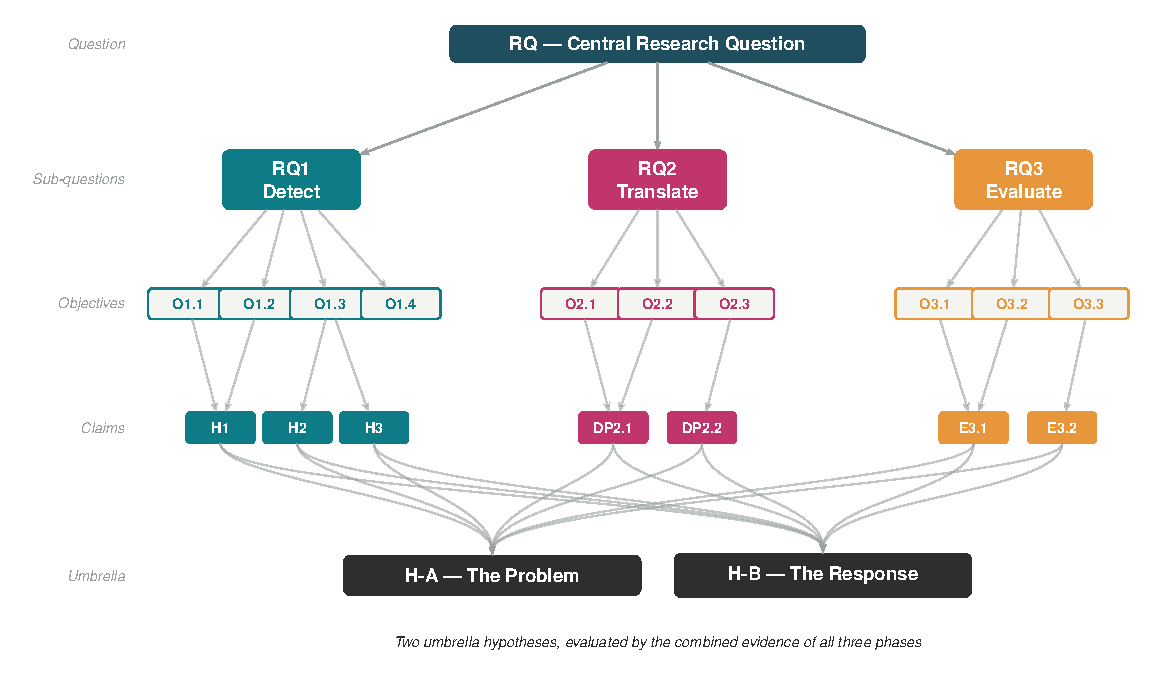
\includegraphics[width=\textwidth]{figures/research_questions/rq_tree_preview.pdf}
    \caption[Structure of the research questions, objectives, claims and umbrella hypotheses.]{\textbf{The
    architecture of the research programme.} The central research question branches into three
    sub-questions along the detect--translate--evaluate arc. Each sub-question generates its objectives
    (O1.1--O1.4, O2.1--O2.3, O3.1--O3.3), which give rise to the claims appropriate to their epistemic
    character: directional hypotheses (H1--H3), design propositions (DP2.1--DP2.2) and empirical
    expectations (E3.1--E3.2). All three claim groups converge on the two umbrella hypotheses, H-A (the
    problem) and H-B (the response), assessed not by any single instrument but by the combined evidence
    of the whole programme.}
    \label{fig:rq-tree}
\end{figure}

% -------------------------------------------------------------------------
\section{Fattibilità e disciplina dell'ambito}
\label{sec:rq-feasibility}

La fattibilità poggiava su infrastruttura, tempo e controllo dell'ambito. La fase analitica ha attinto al record RAPID e all'ensemble Copernicus, elaborati e riportati nel Capitolo~\ref{ch:data_pipeline}, realizzando O1.1--O1.3, con O1.4 lasciato come confine di ambito. La fase empirica ha richiesto una preparazione modesta: un questionario di venti minuti somministrato a venticinque partecipanti non specialisti, assegnati casualmente a due gruppi --- una condizione statica convenzionale come controllo e una condizione esperienziale costruita su visualizzazioni interattive guidate dal machine learning. Un campione di queste dimensioni si addice a uno studio esplorativo di primo stadio volto a individuare pattern iniziali nel modo in cui i partecipanti comprendono il sistema, anziché sostenere un'inferenza su scala di popolazione statisticamente potente \citep{braunclarke2006, smithmcgannon2018, malterud2016}. La fase di design è stata la principale impresa tecnica, sviluppata lungo i Capitoli~\ref{ch:methodology} e~\ref{ch:translate}.

Il tempo è stato il vincolo principale, perciò la parte più rischiosa --- costruire la condizione esperienziale --- è avvenuta una volta assestato il testo circostante. Mantenere l'ambito ristretto è stata una scelta metodologica: la previsione è stata lasciata da parte per tenere la tesi sulla rappresentazione anziché sulla predizione \citep{sonnewald2021}, il prototipo è rimasto un artefatto di ricerca, e lo studio è rimasto principalmente esplorativo. Due piani di riserva hanno mantenuto coerente la tesi: se lo studio fosse andato in ritardo, i capitoli analitici e di design sarebbero stati autosufficienti; e se la costruzione fosse fallita, la grammatica di design avrebbe comunque contato come contributo (O2.2). La tesi è ambiziosa ma focalizzata --- ogni obiettivo commisurato al tempo disponibile, ogni affermazione all'evidenza che può reggere.

\begin{table}[!ht]
    \centering
    \small
    \setlength{\tabcolsep}{5pt}
    \renewcommand{\arraystretch}{1.25}
    \caption{Allineamento tra le tre sotto-domande e la struttura operativa della tesi, incluso come ciascuna è validata e rispetto a quale criterio.}
    \label{tab:alignment}
    \begin{tabular}{
        @{}
        >{\RaggedRight\arraybackslash}p{2.7cm}
        >{\RaggedRight\arraybackslash}p{3.7cm}
        >{\RaggedRight\arraybackslash}p{3.7cm}
        >{\RaggedRight\arraybackslash}p{3.7cm}
        @{}
    }
        \toprule
        & \textbf{RQ1 --- Rilevare}
        & \textbf{RQ2 --- Tradurre}
        & \textbf{RQ3 --- Valutare} \\
        \midrule
        \makecell[l]{\textbf{Carattere}\\\textbf{epistemico}}
            & Analitico, comparativo, esplorativo
            & Progettuale, generativo
            & Empirico, qualitativo, comparativo \\[0.5em]

        \textbf{Capitoli}
            & Cap.~\ref{ch:background}, Cap.~\ref{ch:data_pipeline}
            & Cap.~\ref{ch:methodology}, Cap.~\ref{ch:translate}
            & Cap.~\ref{ch:methodology}, Cap.~\ref{ch:userstudy}, Cap.~\ref{ch:results} \\[0.5em]

        \textbf{Obiettivi}
            & O1.1--O1.4
            & O2.1--O2.3
            & O3.1--O3.3 \\[0.5em]

        \textbf{Affermazioni}
            & H1, H2, H3
            & DP2.1, DP2.2
            & E3.1, E3.2 \\[0.5em]

        \textbf{Materiale}
            & Osservazioni RAPID, ensemble di rianalisi Copernicus
            & Strutture latenti recuperate in RQ1
            & Condizioni prodotte in RQ2; partecipanti non specialisti \\[0.5em]

        \makecell[l]{\textbf{Metodo di}\\\textbf{validazione}}
            & Analisi comparativa dei modelli: PCA vs.\ autoencoder a dimensionalità pari; EWS con correzione per pseudo-replicazione; Isolation Forest
            & Costruzione design-science rispetto alla grammatica (Tabella~\ref{tab:design-grammar}); audit di provenienza condivisa della provenienza allineata
            & Studio tra soggetti, venticinque partecipanti non specialisti (dodici controllo, tredici sperimentale), assegnati casualmente alle condizioni statica di controllo ed esperienziale interattiva guidata dal ML; valutazione tramite questionario e analisi esplorativa \\[0.5em]

        \makecell[l]{\textbf{Criterio di}\\\textbf{successo}}
            & Scarto latente $\leq$ errore di ricostruzione; trend nullo correttamente identificato, non forzato
            & Ogni valore a schermo tracciabile al bundle; condizioni equivalenti per costruzione della provenienza
            & Il gruppo sperimentale articola struttura che il gruppo di controllo non articola, nella descrizione spontanea --- valutato per scena, poiché il criterio può essere soddisfatto per alcune strutture e non per altre \\[0.5em]

        \textbf{Output}
            & Analisi della struttura latente; risultato nullo EWS; caratterizzazione delle anomalie
            & Tre condizioni di rappresentazione; grammatica di design documentata
            & Risposte anonimizzate; analisi deduttiva a codebook rispetto a una griglia definita a priori; confronto descrittivo tra i due gruppi \\[0.5em]

        \textbf{Ancoraggio SDG}
            & 13 (Lotta al cambiamento climatico), 14 (La vita sott'acqua)
            & 4 (Istruzione di qualità), 13
            & 4, 13 \\[0.5em]

        \makecell[l]{\textbf{Disciplina}\\\textbf{dell'ambito}}
            & Previsione LSTM rinviata a lavori futuri
            & Prototipo di ricerca, non artefatto di produzione
            & Confronto esplorativo a due gruppi; prevalentemente qualitativo, non statisticamente potente \\
        \bottomrule
    \end{tabular}
\end{table}

% =========================================================================
% CAPITOLO 3 — RASSEGNA DELLA LETTERATURA
% =========================================================================

\chapter{Rassegna della letteratura}
\label{ch:literature}


\noindent
{\rmfamily\itshape
\begin{tabular}[t]{@{}l@{\hspace{0.3cm}}p{12.5cm}@{}}
\textls[50]{\textbf{Trattati:}} &
\textls[50]{Fondamenti teorici · Percezione del rischio e limiti cognitivi · Benchmark attuali ·
Rappresentazione incarnata e immersiva · Principi di design · Vuoti nella letteratura}
\end{tabular}
}

\vspace{0.5cm}

Questo capitolo esamina la letteratura su cui la tesi è costruita. Tre filoni definiscono il problema: la psicologia della percezione del rischio climatico, la scienza cognitiva dei sistemi dinamici e la valutazione empirica della visualizzazione del clima. Due forniscono la risposta: la rappresentazione incarnata e immersiva, e il machine learning usato in modo rappresentativo anziché predittivo. Un sesto filone traduce la teoria in una grammatica di design, e una sezione conclusiva nomina il vuoto che la tesi occupa.

% -------------------------------------------------------------------------
\section{Barriere psicologiche alla percezione del rischio climatico}
\label{sec:psych-barriers}

Il Capitolo~\ref{ch:introduction} ha introdotto l'\emph{ipotesi del deficit di informazione} e l'evidenza contraria \citep{kellstedt2008, kahan2015}.\footnote{In \citet{kellstedt2008} la relazione inversa tra conoscenza e preoccupazione è sopravvissuta ai controlli per affiliazione politica e fattori demografici, indicando un genuino effetto cognitivo-culturale anziché un fattore confondente.} Ciò che conta qui è \emph{perché} fallisce, perché è a questo che il design deve rispondere: l'informazione conta, ma il suo effetto è mediato da meccanismi cognitivi e culturali che i formati standard non hanno mai affrontato.

Il resoconto più influente di questo fallimento è \citet{stoknes2015}, che nomina cinque barriere --- \emph{distanza}, \emph{catastrofismo}, \emph{dissonanza}, \emph{negazione} e \emph{identità} --- che hanno organizzato gran parte del lavoro successivo.\footnote{In breve: \emph{distanza} (il cambiamento climatico appare spazialmente, temporalmente e socialmente remoto), \emph{catastrofismo} (l'inquadramento catastrofista innesca l'evitamento), \emph{dissonanza} (il divario credenza--comportamento si risolve aggiustando la credenza), \emph{negazione} (disimpegno autoprotettivo) e \emph{identità} (le posizioni sul clima segnalano l'appartenenza a un gruppo).} Le barriere si intrecciano anziché agire singolarmente \citep{vanderlinden2015}, e il pubblico si stratifica in gruppi le cui barriere si attivano in modo diverso, perciò nessuna singola strategia le serve tutte \citep{leiserowitz2021}. La visualizzazione convenzionale non le ha dissolte, e la ragione è strutturale: le immagini più usate per comunicare il cambiamento climatico o rafforzano la distanza che i comunicatori sperano di colmare o innescano la risposta di catastrofismo che sopprime il coinvolgimento \citep{cornerclimate2015, nicholsoncole2005}, e i formati che non danno al lettore alcun ruolo attivo rendono costantemente meno di quelli che glielo danno \citep{ojala2023}. Aggiungere precisione a un grafico a linee non apre alcun ruolo di questo tipo --- la sua retorica implicita del \emph{ecco il fatto} non lascia al lettore alcun punto su cui stare. La letteratura punta quindi verso rappresentazioni che trattano il lettore come partecipante attivo nella costruzione del significato \citep{marlon2019, morris2019}, che è la direzione che questa tesi persegue, con il machine learning come substrato.

% -------------------------------------------------------------------------
\section{La scienza cognitiva dei sistemi dinamici e complessi}
\label{sec:cognitive-science}

Sotto questi filtri culturali si trova una barriera indipendente da essi: i limiti strutturali della mente nel ragionare su sistemi di accumulo, retroazione e ritardo. Sono caratteristiche stabili dell'architettura cognitiva, non lacune che un insegnamento migliore potrebbe colmare, e qualsiasi rappresentazione che le ignori fallirà per quanto bene sia calibrata psicologicamente.

L'evidenza più forte è \citet{sterman2008}, i cui esperimenti mostrano che perfino adulti matematicamente competenti commettono errori sistematici su elementari problemi di stock e flusso. Mostrato uno scenario in cui la CO\textsubscript{2} atmosferica si stabilizza, e chiesto di tracciare il percorso delle emissioni coerente con esso, la maggior parte viola il bilancio di massa --- facendo corrispondere la forma dell'uscita a quella dell'ingresso anziché ragionare sulla differenza tra flusso in entrata e in uscita.
\footnote{Negli studi di Sterman l'84\% dei partecipanti molto istruiti --- dottorandi del MIT, ingegneri, partecipanti con formazione in analisi matematica --- ha commesso questo errore, indicando un limite di rappresentazione anziché di aritmetica.} \citet{cronin2009} ha trovato lo stesso in forma più netta: chiesto di tracciare uno stock dal suo flusso in entrata e in uscita, i partecipanti hanno confuso i tassi con i livelli e trattato il sistema dinamico come statico, anche quando possedevano l'apparato matematico per risolverlo. Dato solo un grafico, la mente non costruisce spontaneamente lo scenario dinamico che il grafico raffigura.

% ============================================================
% Sterman (2008) climate stabilization task -- original figures
% extracted from the Science article as vector PDF crops.
%
% Source crops kept alongside in figures/literature/:
%   sterman_scenario.pdf, sterman_task.pdf, sterman_response.pdf
% (the composed panel below is what actually gets included)
% ============================================================

\begin{figure}[htbp]
    \centering
    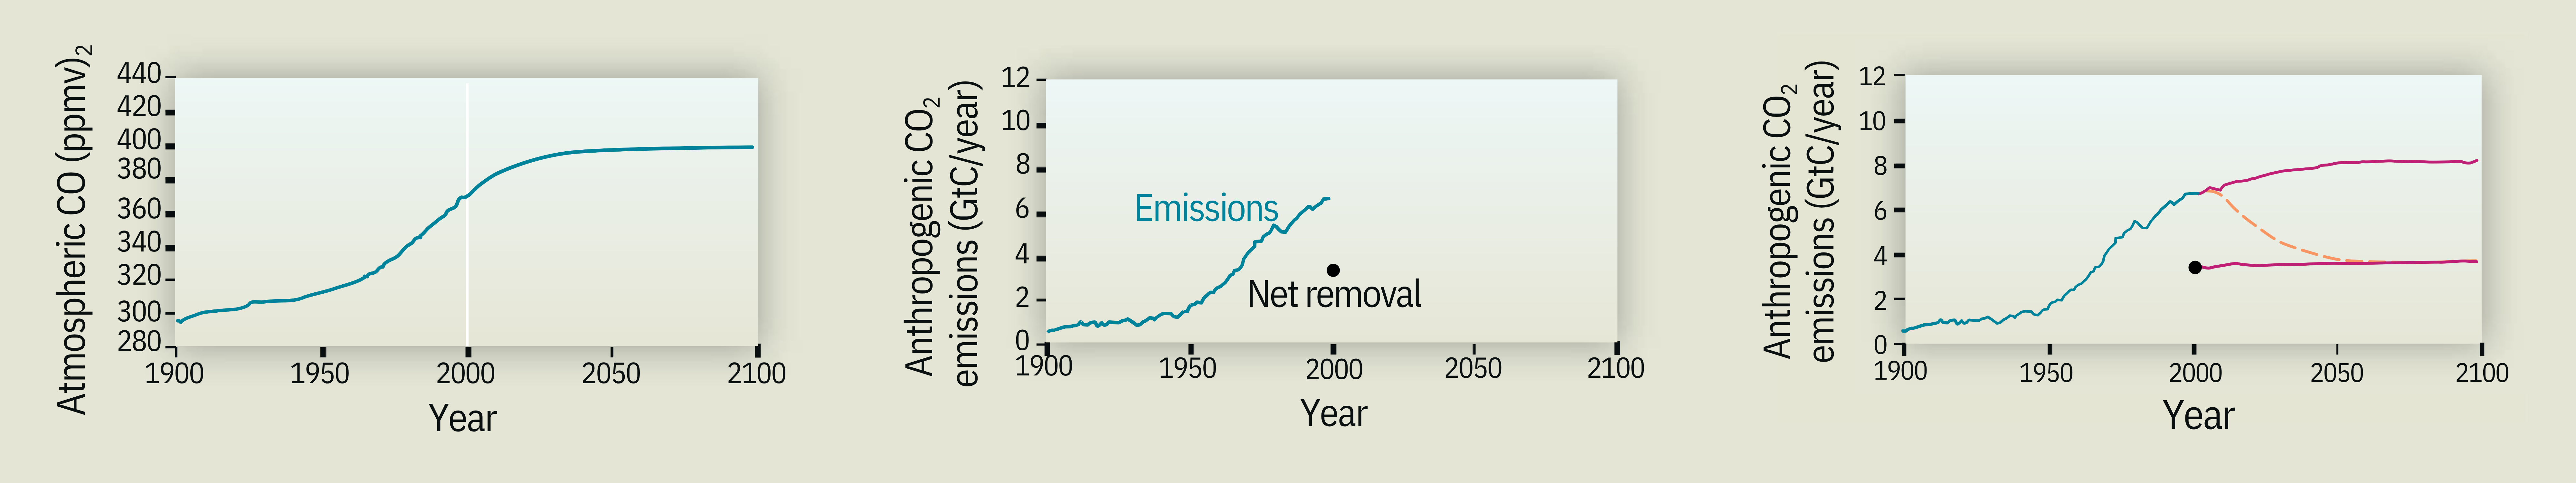
\includegraphics[width=\textwidth]{figures/literature/sterman_panel.png}
    \caption[The climate stabilization task]{The climate stabilization
    task. (a)~The scenario presented to participants: atmospheric
    CO\textsubscript{2} concentration rises gradually to 400~ppmv and
    stabilizes by 2100. (b)~The stock--flow information provided:
    anthropogenic CO\textsubscript{2} emissions from 1900 to 2000 (the
    inflow) and current net removal by oceans and biomass (the
    outflow), with emissions roughly double net removal. (c)~A typical
    response: participants erroneously sketch future emissions that
    match the shape of the CO\textsubscript{2} trajectory
    (pattern-matching heuristic), while mass balance requires emissions
    to fall until they equal net removal (dashed line). Reprinted from
    \citet{sterman2008}.}
    \label{fig:sterman-panel}
\end{figure}

La teoria del carico cognitivo spiega perché \citep{sweller1988, swellervanmerrienboer2019}: la memoria di lavoro è strettamente limitata, e un'immagine statica di un sistema dinamico chiede al lettore di animare mentalmente ciò che l'immagine non anima --- un onere che si aggiunge al dominio stesso. \citet{ware2021} sostiene che una visualizzazione comunicativa deve abbassare questa richiesta di simulazione interna rendendo la struttura dinamica percettivamente disponibile. Un terzo filone guarda avanti: \citet{tversky2019}, sintetizzando quattro decenni di lavoro, mostra che ragionare su processi complessi è fondamentalmente spaziale, compreso attraverso schemi corporei e cinestesici. Se ragionare sulle dinamiche è spazialmente incarnato, le strategie con maggiori probabilità di successo arruolano la cognizione spaziale e cinestesica del lettore --- la proposizione che organizza il resto del capitolo.

% -------------------------------------------------------------------------
\section{Valutazione empirica della visualizzazione del clima}
\label{sec:empirical-viz}

Ciò che è stato misurato su come le visualizzazioni del clima vengono recepite rivela un'asimmetria metodologica: il campo è ricco di studi su ciò che il pubblico \emph{preferisce} e scarso di studi su ciò che \emph{comprende} --- il vuoto che questa tesi affronta. La rassegna più sistematica ha rilevato che i formati standard --- grafici a linee, mappe coropletiche, grafici spaghetti d'ensemble --- sono mal calibrati rispetto alle risorse cognitive del loro pubblico, anche tra lettori esperti di policy \citep{harold2016}. Mostrati un grafico di proiezione dell'IPCC, tali lettori vedono molta incertezza ma la attribuiscono ai modelli, trascurando l'incertezza di scenario che gli stessi intervalli contengono \parencite{mcmahon2015}. In modo più rivelatore, le visualizzazioni che le persone \emph{preferiscono} non sono quelle che producono la più alta \emph{comprensione}: le persone scelgono display più ricchi e realistici anche quando questi le rallentano e ne abbassano l'accuratezza \parencite{hegarty2012}. Ottimizzare per la preferenza rischia quindi di produrre ciò che \citet{sheppard2015} chiama \emph{visualizzazioni consolatorie} --- immagini accolte calorosamente e comprese male.

Questo poggia su una matura scienza della codifica visiva su cui il Capitolo~\ref{ch:translate} attinge direttamente. Bertin ha individuato l'insieme finito di \emph{variabili visive} attraverso cui qualsiasi segno codifica dati \citep{bertin1983}; \citet{clevelandmcgill1984} le ha ordinate per accuratezza di decodifica, con la posizione lungo una scala comune giudicata assai più accuratamente di lunghezza, angolo, area o colore; e \citet{munzner2014} ha trasformato questo nella regola di design dell'\emph{efficacia} --- assegnare l'informazione più importante al canale decodificato con maggiore accuratezza. \citet{ware2021} fonda la stessa regola nella percezione pre-attentiva. La codifica, in breve, è prestazione percettiva misurata, non gusto.

% ============================================================
% Cleveland & McGill (1984) perceptual hierarchy
% Vector PDF figure imported from the figures/ directory.
%
% Requires:
%   cleveland_preview.pdf
%
% (\graphicspath{{figures/}} is already defined in main.tex)
% ============================================================

\begin{figure}[!ht]
    \centering
    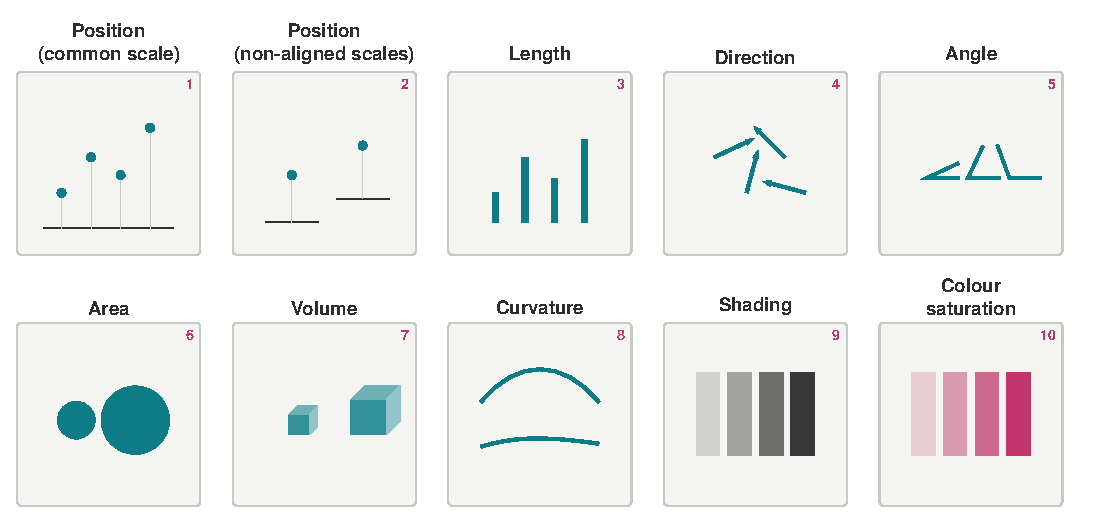
\includegraphics[width=\textwidth]{figures/literature/cleveland_preview.pdf}
    \caption[The Cleveland \& McGill hierarchy of perceptual tasks.]{\textbf{The hierarchy of elementary perceptual tasks, after \citet{clevelandmcgill1984}.}
    Encodings are ordered by decoding accuracy, from most accurate (1, position on
    a common scale) to least accurate (10, colour saturation). The ranking is
    empirical, not aesthetic: it reflects how accurately people extract a
    quantitative value from each visual channel. It underlies design-grammar
    principle~P0 (Table~\ref{tab:design-grammar}) --- assign the most important
    variable to the most accurately decoded channel --- and principle~P1, which
    places continuous magnitude on spatial position.}
    \label{fig:perceptual-hierarchy}
\end{figure}

L'incertezza è dove la codifica convenzionale fallisce di più, e dove questa tesi si discosta di più dalla convenzione. Barre d'errore e bande ombreggiate sono lette male dai non specialisti, che trattano una banda come un bordo netto \citep{spiegelhalter2017}; \citet{padilla2018} spiegano perché, mostrando che le codifiche statiche dell'incertezza sovraccaricano la memoria di lavoro, per cui gli osservatori ripiegano su euristiche che scartano l'incertezza. L'alternativa meglio supportata è \emph{animarla}: gli Hypothetical Outcome Plots mostrano possibili esiti in sequenza, lasciando che l'osservatore senta la dispersione invece di decodificare una banda, e osservatori non addestrati li giudicano più accuratamente delle barre d'errore \citep{hullman2015hops, kale2019hops}. Questo autorizza la mossa centrale della tesi --- rendere l'incertezza una qualità percettiva sentita anziché un numero tra parentesi.

Questi limiti sono visibili nel modo in cui l'AMOC stessa è comunicata, il che fissa la condizione di controllo dello studio. Nel record scientifico e pubblico compare quasi interamente come grafici a linee del trasporto in sverdrup, proiezioni d'ensemble mostrate come dispersione ombreggiata e indici ``fingerprint'' ricostruiti, con il Gruppo intergovernativo sui cambiamenti climatici (IPCC) che aggiunge qualificatori verbali come ``molto probabilmente si indebolirà'' \citep{caesar2018, ipcc2021}. Ciascuno è limitato esattamente come le sezioni precedenti prevedono: la curva statica raffigura un sistema dinamico nel suo stato finale; la banda ombreggiata codifica l'incertezza nel modo che si è mostrato essere frainteso; i qualificatori verbali chiedono a un non specialista di tenere in memoria di lavoro un giudizio probabilistico di soglia senza alcun supporto percettivo; e nessuno trasmette la non linearità che definisce un elemento di tipping. La baseline convenzionale comunica entità e tendenza ma non dinamiche, non linearità o incertezza --- proprio ciò che la condizione esperienziale è progettata per migliorare, e ricostruirla fedelmente è ciò che rende equo il confronto nel Capitolo~\ref{ch:userstudy}.

% -------------------------------------------------------------------------
\section{Cognizione incarnata e rappresentazione immersiva}
\label{sec:embodied-viz}

Se la risposta è arruolare la cognizione spaziale e corporea, tre tradizioni correlate mostrano come. Il fondamento filosofico è \citet{lakoff1999}: i concetti astratti attraverso cui ragioniamo sui sistemi --- accelerazione, retroazione, stabilità, tipping --- sono estensioni dell'esperienza corporea e spaziale, non logica disincarnata, e \citet{kirsh2013}, passando in rassegna la letteratura sulla cognizione incarnata, sostiene che le persone in grado di gesticolare e muoversi mentre ragionano su processi complessi sono meglio supportate di quelle vincolate a un'ispezione statica. La \emph{physicalisation dei dati} \citep{jansen2015} è nata da questo, codificando informazioni per l'esplorazione attraverso tatto e vista; l'informazione codificata in un grafico fisico viene anche dimenticata più lentamente della stessa informazione su uno schermo \parencite{stusak2015}. Parallelamente, il \emph{data humanism} sostiene che una rappresentazione narrativa e d'autore coinvolga i lettori più profondamente di un'estetica di distaccata astrazione \citep{lupi2017, segel2010}. La terza, l'\emph{immersive analytics}, sostiene che le interfacce spazialmente consapevoli offrano affordance che lo schermo piatto non può, adatte a dati la cui struttura è spaziale o dinamica \citep{marriott2018}.\footnote{Le valutazioni formali dell'immersive analytics restano limitate, e l'evidenza attuale più forte riguarda compiti spaziali e temporali tridimensionali anziché sistemi complessi astratti. L'allineamento teorico con la scienza cognitiva della \S\ref{sec:cognitive-science} è nondimeno diretto.} Il rendering basato su browser e l'audio in tempo reale portano un sottoinsieme utile di queste affordance alla portata di un singolo progetto di ricerca senza hardware specializzato, che è l'apertura che questa tesi coglie. Insieme, queste tradizioni sostengono un'unica affermazione: la difficoltà di comunicare sistemi climatici complessi non è affrontabile entro il paradigma convenzionale, e indica di trattare il lettore come partecipante attivo e incarnato.

% -------------------------------------------------------------------------
\section{Il machine learning come substrato di rappresentazione}
\label{sec:ml-climate}

Il machine learning per la scienza del clima è ormai vasto, ma la sua agenda dominante è \emph{predittiva}: prevedere variabili, rilevare anomalie, parametrizzare processi fisici, fare downscaling dell'output dei modelli \citep{reichstein2019, sonnewald2021}. La letteratura sull'AMOC rispecchia questo, applicando il machine learning soprattutto per rilevare segnali di preallarme o prevedere la variabilità \citep{boers2021, ditlevsen2023}. Questo lavoro è prezioso, ma è orientato quasi interamente a nuovi risultati per un pubblico esperto, lasciando inesplorata una domanda adiacente: che cosa contribuisce il machine learning quando l'obiettivo non è un nuovo risultato ma rendere un oggetto scientifico esistente \emph{intelligibile ai non specialisti}.

La distinzione merita di essere enunciata con precisione. Una rete che prevede il trasporto dell'AMOC produce una nuova capacità, giudicata in unità condivise --- correlazione, errore, calibrazione. Un'analisi di riduzione della dimensionalità dello stesso record produce una rappresentazione latente il cui valore sta altrove: in quali poche coordinate spiegano gran parte della variabilità, e cosa significano fisicamente. La tesi usa il machine learning in questo secondo ruolo, \emph{rappresentativo}. L'affermazione non è che la struttura verticale dell'AMOC sia nuova --- è coerente con decenni di oceanografia \citep{hannachi2007, buckley2016} --- ma che, una volta recuperata, può diventare il sistema di coordinate attraverso cui l'AMOC è resa disponibile alla percezione. La letteratura che tratta il machine learning in questo modo è esigua ma reale: si è sostenuto che le rappresentazioni latenti siano legittimi oggetti epistemologici in fisica \citep{iten2020}, e la ricerca di analisi visiva tratta lo spazio latente di un modello come il substrato attraverso cui un analista costruisce comprensione \citep{sacha2018}. Il machine learning è stato occasionalmente rivolto alla comunicazione pubblica del clima, per esempio per generare immagini di future inondazioni in luoghi che le persone conoscono \parencite{schmidt2022}, ma non per rendere percepibile la struttura latente di un sistema climatico. Questo è il vuoto.

% -------------------------------------------------------------------------
\section{Grammatica di design}
\label{sec:design-grammar}

Le sezioni precedenti mostrano perché la visualizzazione convenzionale spesso fallisce e perché un approccio incarnato offre un'alternativa; non spiegano ancora \emph{come} un tale approccio debba essere progettato. Questa sezione colma quel vuoto derivando principi di design dalla letteratura sopra, ciascuno dei quali collega una proprietà del sistema a un canale percettivo, così che le scelte nel Capitolo~\ref{ch:translate} siano informate anziché estetiche --- ognuna tracciabile a un fondamento e difendibile di per sé.

Il principio capostipite è la regola dell'efficacia stabilita nella \S\ref{sec:empirical-viz}: l'informazione più importante dovrebbe essere assegnata al canale visivo decodificato con maggiore accuratezza \citep{bertin1983, clevelandmcgill1984, munzner2014}. I restanti principi seguono applicandola alle caratteristiche dei sistemi complessi: l'entità attraverso la posizione spaziale, il cambiamento nel tempo attraverso il movimento, le anomalie attraverso densità o texture, l'incertezza attraverso variazione controllata anziché intervalli statici, e l'informazione ordinata secondaria attraverso il suono. Queste mappature sono enunciate come principi generali applicabili a sistemi invisibili oltre l'AMOC. La Tabella~\ref{tab:design-grammar} riassume la grammatica; il Capitolo~\ref{ch:translate} la applica alle proprietà del sistema recuperate nel Capitolo~\ref{ch:data_pipeline}.

La grammatica colloca anche la tesi entro il più ampio campo della rappresentazione esperienziale dei dati. La pratica della data art esplora già come strutture nascoste da modelli computazionali possano diventare esperienze percettive: lo studio fuse*, per esempio, tratta gli spazi latenti dei modelli generativi come ambienti di trasformazione continua.\footnote{fuse*, \emph{Artificial Botany} e opere correlate, \url{https://fuseworks.it}. Lo studio descrive il proprio interesse come la ``dimensione intermedia'' dello spazio latente, esplorata come spazio di esplorazione espressiva anziché come rappresentazione diretta di un sistema misurato.} Questi approcci condividono un'assunzione con questa tesi --- che la struttura computazionale possa diventare qualcosa da esperire, non solo da analizzare --- ma non verificano se un pubblico \emph{comprenda} qualcosa come risultato. Il contributo qui è il passo che la pratica omette: fondare ciascuna scelta percettiva nei principi della Tabella~\ref{tab:design-grammar}, e verificare in modo comparativo se il risultato sostenga tanto un'esperienza significativa quanto una comprensione misurabile.

% ============================================================
% fuse* Artificial Botany (2019) -- original figure
% extracted from the studio's website.
% ============================================================

\begin{figure}[htbp]

    \centering

    \includegraphics[width=\textwidth]{figures/literature/fuse\_artificial\_botany.jpg}

    \caption[\emph{Artificial Botany} by fuse\textsuperscript{*}]{
        \emph{Artificial Botany} by fuse\textsuperscript{*}. The work explores the latent space of generative networks as a terrain of morphing forms.
    }

    \label{fig:fuse-artificial-botany}

\end{figure}

\begin{table}[!ht]
    \centering
    \small
    \caption[Una grammatica di design per la rappresentazione esperienziale dei sistemi complessi.]{\textbf{Una grammatica di design per la rappresentazione esperienziale dei sistemi complessi.}
             Ogni riga mappa una \emph{proprietà del sistema} su un \emph{canale percettivo} attraverso un
             \emph{principio cognitivo} documentato, ancorato a una \emph{fonte}. P0 è il principio
             capostipite --- l'accuratezza di decodifica è ordinata, non uniforme --- da cui P1--P5 seguono
             per applicazione alle proprietà di un sistema complesso. La grammatica è qui enunciata in
             forma generale e trasferibile; la sua applicazione alle specifiche caratteristiche dell'AMOC
             recuperate nel Capitolo~\ref{ch:data_pipeline} (intensità latente, transizioni, anomalie,
             incertezza d'ensemble) è sviluppata nel Capitolo~\ref{ch:translate}. Movimento (P2),
             incertezza animata (P4) e suono (P5) sono i canali attraverso cui questa
             grammatica va oltre la visualizzazione statica convenzionale.}
    \label{tab:design-grammar}
    \begin{tabular}{@{}p{0.5cm}p{2.5cm}p{2.9cm}p{3.3cm}p{2.3cm}@{}}
        \toprule
        & \textbf{Proprietà del sistema} & \textbf{Canale percettivo} & \textbf{Principio cognitivo} & \textbf{Fonte} \\
        \midrule
        P0 & Importanza relativa delle variabili
           & Canale più accurato per la variabile più importante
           & Efficacia: l'accuratezza di decodifica è ordinata, non uniforme
           & \citet{bertin1983, clevelandmcgill1984, munzner2014} \\[0.4em]
        P1 & Entità / intensità (ordinata, continua)
           & Posizione spaziale su un asse comune
           & La posizione è il canale decodificato con maggiore accuratezza per dati ordinati
           & \citet{clevelandmcgill1984, munzner2014} \\[0.4em]
        P2 & Dinamiche / cambiamento nel tempo
           & Movimento reale
           & La mente non può animare mentalmente un fotogramma statico; ragionare sul processo è spaziale, e il movimento è tracciato in modo pre-attentivo
           & \citet{sterman2008, cronin2009, tversky2019, ware2021} \\[0.4em]
        P3 & Anomalia / scostamento dal regime
           & Cambiamento locale di densità o texture
           & L'irregolarità attira l'attenzione dal basso senza bisogno di legenda
           & \citet{bertin1983, ware2021} \\[0.4em]
        P4 & Incertezza
           & Variabilità animata (movimento, densità, suono), non una banda statica
           & Le bande statiche sovraccaricano la memoria di lavoro; gli esiti animati sono giudicati più accuratamente
           & \citet{padilla2018, hullman2015hops, kale2019hops} \\[0.4em]
        P5 & Variabile ordinata secondaria
           & Suono (altezza, ritmo, timbro)
           & I canali uditivi portano dati ordinati in parallelo, senza affollamento visivo
           & \citet{hermann2011} \\
        \bottomrule
    \end{tabular}
\end{table}

% -------------------------------------------------------------------------
\section{Sintesi: l'intersezione che questa tesi occupa}
\label{sec:literature-synthesis}

Letti come un unico argomento, i filoni convergono su una proposizione che nessuno enuncia da solo. L'informazione sul clima è filtrata attraverso barriere psicologiche che i formati convenzionali non affrontano (\S\ref{sec:psych-barriers}), aggravate da limiti strutturali al ragionare sulle dinamiche a partire da immagini statiche (\S\ref{sec:cognitive-science}). La visualizzazione del clima è stata valutata per lo più per preferenza anziché per comprensione, benché esista una matura scienza della codifica su cui fondare scelte migliori (\S\ref{sec:empirical-viz}). Le tradizioni incarnata e immersiva mostrano la direzione di una risposta ma hanno raramente raggiunto la comunicazione del clima (\S\ref{sec:embodied-viz}), e il machine learning è avanzato in modo predittivo, lasciando quasi inesplorato il ruolo rappresentativo della struttura latente (\S\ref{sec:ml-climate}). La grammatica di design (\S\ref{sec:design-grammar}) mostra che questi filoni possono essere combinati in principi operativi --- ma nessun lavoro esistente l'ha fatto e ne ha verificato il risultato.

L'intersezione è stretta ed empiricamente non popolata, definita da cinque impegni: un sistema climatico la cui invisibilità e non linearità ne fanno una prova da sforzo \citep{lenton2008, armstrongmckay2022}; un trattamento di machine learning che recupera struttura latente anziché fare previsioni \citep{sonnewald2019, iten2020}; una tradizione di design che tratta il lettore come incarnato e attivo \citep{lakoff1999, jansen2015, marriott2018}; un confronto tra formati convenzionali ed esperienziali \parencite{harold2016, hegarty2012}; e una valutazione qualitativa ed esplorativa appropriata a un fenomeno non ancora maturo per un'inferenza su scala di popolazione \citep{braunclarke2006}. Nessuno studio esaminato soddisfa tutti e cinque congiuntamente. Il vuoto non è l'assenza di un singolo impegno ma l'assenza della loro integrazione --- e integrarli, sull'AMOC come caso, è ciò che i capitoli che seguono intraprendono.

% =========================================================================
% CAPITOLO 4 — INQUADRAMENTO SCIENTIFICO
% =========================================================================

\chapter{Inquadramento scientifico}
\label{ch:background}

\noindent
{\rmfamily\itshape
\begin{tabular}[t]{@{}l@{\hspace{0.3cm}}p{12.5cm}@{}}
\textls[50]{\textbf{Trattati:}} &
\textls[50]{Sistema fisico · Circolazione termoalina · Bistabilità e tipping · Isteresi ·
Misura e unità · Dati osservativi e rianalisi}
\end{tabular}
}

\vspace{0.5cm}

Questo capitolo spiega che cos'è l'AMOC: come funziona come sistema fisico, perché può passare da uno stato all'altro, come se ne misura l'intensità e quali record esistono. È volutamente breve. Qui è incluso solo ciò che i capitoli successivi usano effettivamente --- ciò che la fase di \emph{rilevamento} scompone e ciò che la fase di \emph{traduzione} deve rendere percepibile.

% -------------------------------------------------------------------------
\section{Il sistema fisico}
\label{sec:bg-physical}

La Atlantic Meridional Overturning Circulation è il nastro trasportatore di calore dell'oceano attraverso l'Atlantico. L'acqua superficiale calda e salata scorre verso nord; nei freddi mari subpolari cede calore all'atmosfera, diventa densa e sprofonda; torna quindi verso sud in profondità come corrente fredda e profonda (Figura~\ref{fig:amoc-schematic}). Questo rovesciamento verticale --- flusso superficiale in un verso, flusso profondo nell'altro --- è guidato da differenze di densità dell'acqua determinate da temperatura e salinità, il processo noto come circolazione termoalina.

% figures/background/amoc_schematic.tex — loads compiled PDF
% Requires \usepackage{graphicx}. Insert with \input{...}.
\begin{figure}[!ht]
    \centering
    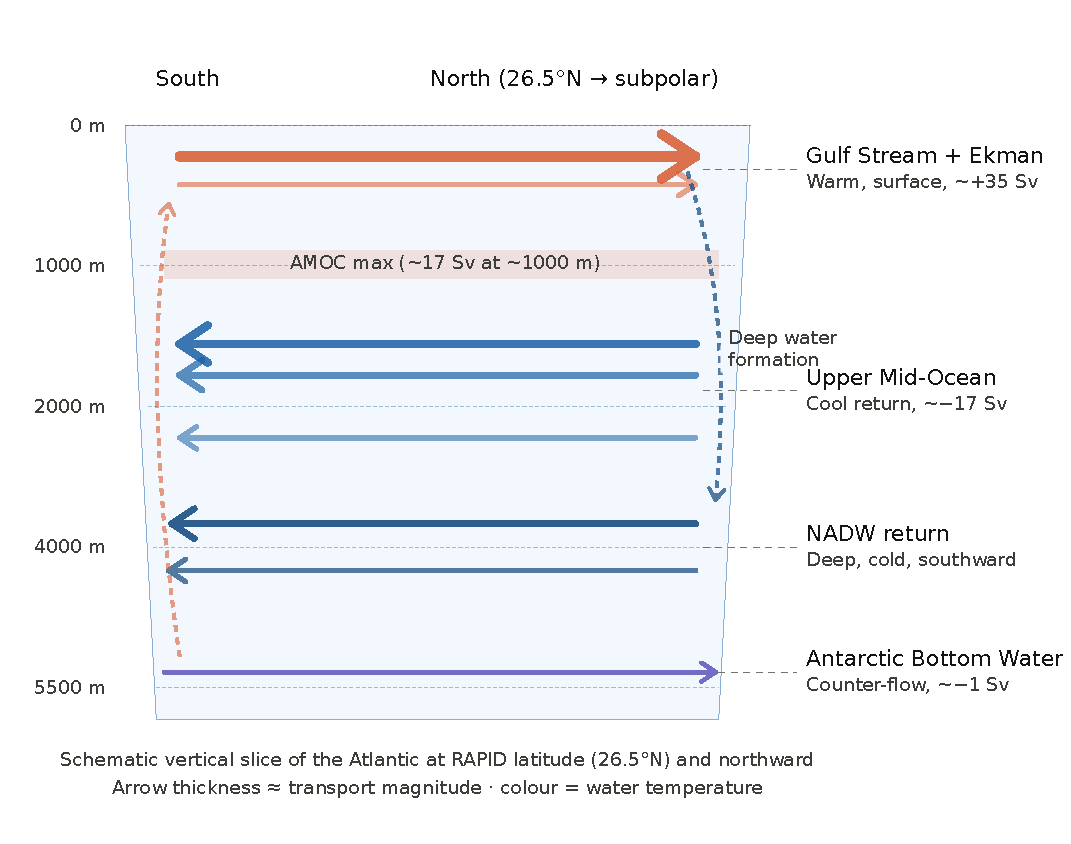
\includegraphics[width=0.9\textwidth]{figures/background/amoc_atlantic_cross_section.pdf}
    \caption[The Atlantic overturning circulation.]{\textbf{The Atlantic
    overturning circulation in cross-section.} Warm surface water flows north
    (orange), releases heat to the atmosphere in the subpolar seas, grows dense
    and sinks, and returns south as a cold deep current (blue). The vertical
    overturning is driven by density differences of temperature and salinity.
    The circulation has no visible surface expression --- the invisibility the
    thesis sets out to address.}
    \label{fig:amoc-schematic}
\end{figure}

La conseguenza è climatica, non meramente oceanografica. Il flusso superficiale verso nord trasporta nel Nord Atlantico dell'ordine di un petawatt di calore --- paragonabile alla produzione di un milione di grandi centrali elettriche --- e gran parte della relativa mitezza dell'Europa nord-occidentale dipende da esso \citep{buckley2016}. Eppure il sistema non ha alcuna superficie che un osservatore possa vedere: è una circolazione nell'interno dell'oceano, estesa su un bacino, che si dispiega su decenni. È proprio questo il divario che la tesi affronta --- un processo di grande portata e di nessuna visibilità quotidiana.

% -------------------------------------------------------------------------
\section{Bistabilità e tipping}
\label{sec:bg-bistability}

Ciò che rende l'AMOC un \emph{elemento di tipping}, anziché un sistema che semplicemente si indebolisce in proporzione al riscaldamento, è un meccanismo di retroazione colto per la prima volta da \citet{stommel1961} in un semplice modello dell'oceano a due scatole.\footnote{Stommel rappresentò l'oceano come due scatole, equatoriale e polare, che si scambiano acqua a un tasso fissato dalla loro differenza di densità. La retroazione di avvezione del sale nelle sue equazioni produce due equilibri stabili per lo stesso forzante esterno --- la firma matematica della bistabilità.} Il meccanismo è un ciclo: il rovesciamento trasporta sale verso nord, il sale mantiene densa l'acqua settentrionale, e l'acqua densa continua a sprofondare, sostenendo il rovesciamento. Si aggiunga abbastanza acqua dolce al Nord Atlantico --- dal ghiaccio che si scioglie, per esempio --- e il ciclo può girare al contrario: acqua più dolce è meno densa, lo sprofondamento si indebolisce, meno sale viene portato a nord, e la circolazione si rallenta ulteriormente da sé.

A causa di questa retroazione, l'AMOC ha due stati stabili --- un rovesciamento vigoroso e uno molto più debole --- per le stesse condizioni. Una spinta graduale può quindi innescare un passaggio brusco, e invertire la spinta non inverte semplicemente il passaggio.

Questa proprietà, chiamata isteresi, è la ragione per cui il comportamento del sistema è non lineare e per cui resiste all'intuizione: causa ed effetto non sono proporzionali. Comunicare quella non linearità, che nessuna curva statica trasmette, è la sfida di rappresentazione al centro di questa tesi.

% -------------------------------------------------------------------------
\section{Misurare la circolazione}
\label{sec:bg-measurement}

Per analizzare l'AMOC, la sua intensità va espressa come numero. Quel numero è il volume d'acqua che il rovesciamento muove, misurato in \emph{sverdrup} (\SI{1}{\sverdrup} = \SI{e6}{\cubic\metre\per\second} --- un milione di metri cubi al secondo).\footnote{Formalmente, la funzione di corrente del rovesciamento integra la velocità verso nord attraverso il bacino e verso il basso dalla superficie; il suo massimo lungo la profondità definisce il trasporto AMOC a una data latitudine.} Un tipico rovesciamento alle medie latitudini si attesta su circa \SIrange{15}{20}{\sverdrup}.

Cosa cruciale per ciò che segue, la circolazione non è un singolo numero ma un \emph{profilo}: il trasporto varia con la profondità, forte vicino alla superficie dove l'acqua calda scorre verso nord, invertendosi in profondità dove l'acqua fredda torna verso sud. Questo profilo verticale, risolto nel tempo, è la materia prima che la fase di \emph{rilevamento} scompone --- l'oggetto da cui il machine learning recupera una struttura latente compatta nel Capitolo~\ref{ch:data_pipeline}.

% -------------------------------------------------------------------------
\section{Dati osservativi}
\label{sec:bg-data}

L'AMOC è osservata direttamente dall'array RAPID-MOCHA-WBTS (Rapid Climate Change --- Meridional Overturning Circulation and Heatflux Array --- Western Boundary Time Series) a \ang{26.5}~nord, una linea di strumenti ormeggiati che attraversa l'Atlantico e che misura il rovesciamento con continuità dal 2004 \citep{frajkawilliams2021, moat2026}. RAPID è l'àncora empirica di questa tesi: un record autentico e continuo di un sistema che in precedenza era stato solo dedotto.

Il suo unico limite è la lunghezza. Due decenni di dati sono pochi rispetto a una circolazione che varia su scale da decenni a secoli, perciò il record osservato non può da solo rivelare il comportamento lento del sistema. Per fornire un contesto più lungo, l'analisi aggiunge l'ensemble Copernicus Marine GREP --- una rianalisi che ricostruisce la circolazione prima del periodo osservativo combinando modelli con dati assimilati, al prezzo di introdurre una dipendenza dai modelli e una dispersione tra i membri dell'ensemble. Quella dispersione non è una mera avvertenza: diventa, nella fase di \emph{traduzione}, la forma grezza di incertezza che la rappresentazione deve rendere percepibile. Insieme, osservazione e rianalisi sono i due insiemi di dati che il capitolo successivo analizza.

% =========================================================================
% CAPITOLO 5 — METODOLOGIA
% =========================================================================

\chapter{Metodologia}
\label{ch:methodology}

\noindent
{\rmfamily\itshape
\begin{tabular}[t]{@{}l@{\hspace{0.3cm}}p{12.5cm}@{}}
\textls[50]{\textbf{Trattati:}} &
\textls[50]{Approccio · Design Science Research · Disegno e flusso della ricerca · Le ipotesi come
motori · Raccolta e analisi dei dati · Triangolazione · Etica della ricerca · Giustificazione}
\end{tabular}
}

\vspace{0.5cm}

Questo capitolo spiega la logica che tiene insieme la tesi: quale approccio di ricerca è stato scelto, perché questa particolare combinazione di metodi, e come i dati diventano, passo dopo passo, una rappresentazione esperienziale che può essere testata. Non ripete le domande di ricerca e le ipotesi esposte nel Capitolo~\ref{ch:rqs}, né i risultati riportati più avanti. Spiega il ragionamento che li connette.

% -------------------------------------------------------------------------
\section{Approccio metodologico}
\label{sec:research-design}

La tesi si chiede se una rappresentazione esperienziale guidata dal machine learning aiuti i non specialisti a comprendere un sistema climatico complesso meglio di una convenzionale. A quella domanda non si può rispondere con la sola analisi o con la sola costruzione: un artefatto va costruito, e il suo effetto misurato. Ciò colloca il lavoro all'interno del \emph{Design Science Research} (DSR), la tradizione concepita per una ricerca il cui contributo centrale è un artefatto costruito e la cui conoscenza deriva dal costruirlo e testarlo \citep{hevner2004, peffers2007}. L'artefatto qui è la rappresentazione esperienziale; la conoscenza è ciò che la sua realizzazione e il suo test rivelano sul trasformare un sistema invisibile in qualcosa che le persone possono percepire.

Il DSR è una famiglia di metodi anziché un'unica ricetta fissa, e questa tesi segue il diffuso modello a sei fasi di \citet{peffers2007}: identificare il problema, definire gli obiettivi, progettare e sviluppare, dimostrare, valutare, comunicare. La tesi si mappa su questo modello attraverso il suo arco \emph{rilevare--tradurre--valutare}. \emph{Rilevare} porta l'identificazione del problema e il recupero del materiale da rappresentare; \emph{tradurre} porta la progettazione e lo sviluppo dell'artefatto; \emph{valutare} porta il suo test con i partecipanti; e la tesi stessa è la comunicazione. L'arco non è una nuova metodologia ma una versione in linguaggio piano di una consolidata, chiamata per ciò che il lavoro fa effettivamente con un sistema climatico.

Entro questa cornice le tre fasi usano strumenti diversi: \emph{rilevare} è quantitativa, \emph{tradurre} è progettuale e \emph{valutare} è uno studio con utenti a metodi misti, prevalentemente qualitativo con supporto quantitativo descrittivo. Questi non sono paradigmi rivali ma tre strumenti per tre stadi di un unico processo di design science, tenuti insieme dal \emph{pragmatismo} --- giudicare la conoscenza da se funzioni per uno scopo anziché da se corrisponda a un'unica realtà fissa.\footnote{Il pragmatismo è l'epistemologia convenzionalmente abbinata al design science e ai metodi misti \citep{peffers2007}. Autorizza a trattare una struttura latente di machine learning come substrato valido per la rappresentazione non perché sia univocamente ``corretta'', ma perché è utile a rendere percepibile un sistema invisibile; e lascia che misurazione quantitativa e resoconti qualitativi contino come evidenza sulla stessa domanda pratica senza forzare l'uno nello stampo dell'altro.}

Una caratteristica del DSR plasma l'intero disegno: un artefatto deve essere valutato, non semplicemente costruito, perché un'utilità affermata ma non mostrata non è un contributo \citep{hevner2004}. È per questo che la domanda centrale è comparativa --- \emph{in che misura}, \emph{rispetto a} una baseline convenzionale --- ed è per questo che la fase di \emph{valutazione} è essenziale.

% -------------------------------------------------------------------------
\section{Disegno della ricerca e flusso di lavoro}
\label{sec:workflow}

La tesi procede come una pipeline in cui l'output di ciascuna fase è l'input della successiva (Tabella~\ref{tab:workflow}): l'analisi recupera un piccolo insieme di coordinate che catturano come il sistema si comporta; quelle coordinate, guidate da principi percettivi documentati, diventano rappresentazioni che un non specialista può esperire; e quelle rappresentazioni sono ciò che poi viene dato ai partecipanti. Ogni freccia di quella catena è un impegno metodologico. L'analisi vincola ciò che può essere onestamente mostrato, e la rappresentazione è esattamente ciò che lo studio verifica --- nulla è aggiunto tra le fasi che la fase precedente non abbia giustificato.

% figures/methodology/tab_workflow.tex — the detect-translate-evaluate workflow
% Requires \usepackage{booktabs}. Shows phase, method, input, output.
\begin{table}[!ht]
    \centering
    \small
    \renewcommand{\arraystretch}{1.3}
    \caption[The detect--translate--evaluate workflow.]{The thesis pipeline. Each
    phase takes the output of the previous one as its input, so that the analysis
    constrains the design and the design is what the evaluation tests.}
    \label{tab:workflow}
    \begin{tabular}{@{}>{\raggedright\arraybackslash}p{2.3cm}>{\raggedright\arraybackslash}p{3.5cm}>{\raggedright\arraybackslash}p{3.2cm}>{\raggedright\arraybackslash}p{3.2cm}@{}}
        \toprule
        \textbf{Phase} & \textbf{Method} & \textbf{Input} & \textbf{Output} \\
        \midrule
        \textbf{Detect}
            & PCA, autoencoder, anomaly \& early-warning analysis
            & RAPID observations; Copernicus reanalysis
            & Interpretable latent structure of the system \\
        \textbf{Translate}
            & Design grammar applied to recovered features; browser-based build
            & Latent structure from \emph{detect}
            & Three representational conditions (static, dynamic, experiential) \\
        \textbf{Evaluate}
            & Two-group study; think-aloud; reflexive thematic analysis
            & Representations from \emph{translate}
            & Evidence on how non-specialists understand the system \\
        \bottomrule
    \end{tabular}
\end{table}

Il filo unico che la attraversa è la \emph{fedeltà}: ciò che l'analisi recupera fissa il limite di ciò che la rappresentazione può affermare. È questo a rendere l'artefatto finale difendibile come traduzione della scienza anziché come illustrazione ispirata a essa.

% -------------------------------------------------------------------------
\section{Le ipotesi come motori metodologici}
\label{sec:hypotheses-drivers}

Le ipotesi e le domande di ricerca sono state formalizzate nel Capitolo~\ref{ch:rqs}. Ciò che conta metodologicamente è che ciascun tipo di affermazione ha deciso il metodo usato per indagarla. Le ipotesi analitiche (H1--H3) chiedono cosa c'è nei dati, perciò sono indagate con analisi quantitativa che può confermarle o ribaltarle. Le proposizioni progettuali (DP2.1--DP2.2) non sono affermazioni vere-o-false ma impegni di design, perciò sono indagate per costruzione e difese rispetto a criteri di design anziché testate per significatività. Le aspettative empiriche (E3.1--E3.2) riguardano come le persone comprendono, perciò sono indagate qualitativamente --- attraverso ciò che i partecipanti scrivono, non attraverso un test statistico che il campione non potrebbe sostenere. Abbinare ciascuna affermazione al tipo di evidenza che può effettivamente reggere è esso stesso una decisione metodologica, e governa ogni scelta che segue.

% -------------------------------------------------------------------------
\section{Metodi di raccolta e analisi dei dati}
\label{sec:data-methods}

\subsection{La fase analitica}
\label{subsec:analytical}

L'analisi attinge a due fonti di diverso status. L'array RAPID-MOCHA-WBTS a \ang{26.5}~nord ha \emph{osservato} direttamente il rovesciamento dal 2004 \citep{frajkawilliams2021, moat2026}; l'ensemble Copernicus GREP è una \emph{rianalisi} che ricostruisce la circolazione più indietro nel tempo, al prezzo di una dipendenza dai modelli e di una dispersione d'ensemble \citep{copernicus_grep}. La distinzione ne governa l'uso: RAPID àncora l'analisi alla misura, la rianalisi fornisce contesto più lungo e la materia prima per l'incertezza. Ogni affermazione è formulata rispettando su quale delle due poggia.\footnote{Trattare un valore ricostruito come se fosse osservato travisarebbe l'evidenza, perciò i due non sono mai confusi. Questo confine è registrato nell'Appendice~\ref{app:ethics}.}

Tre metodi agiscono poi su questi dati, ciascuno scelto per una ragione specifica; i loro risultati compaiono nel Capitolo~\ref{ch:data_pipeline}. L'\emph{analisi delle componenti principali} riduce la struttura verticale ad alta dimensionalità a poche coordinate, scelta perché le sue componenti sono lineari e fisicamente interpretabili --- un requisito qui, dato che queste coordinate diventano il substrato che un non specialista abiterà, e ciò che non si può spiegare non si può difendere. Poiché la PCA è lineare, un \emph{autoencoder non lineare} è addestrato accanto a essa come controllo: se non ricostruisce i dati meglio a dimensionalità pari, la struttura è genuinamente a bassa dimensionalità e le coordinate interpretabili non perdono nulla. Infine, il \emph{rilevamento di anomalie} e l'\emph{analisi dei segnali di preallarme} caratterizzano il record nel tempo --- il primo per trovare gli eventi che una rappresentazione dovrebbe trasmettere, il secondo per testare segnali di una transizione in avvicinamento, con il test di significatività corretto per la dipendenza delle finestre sovrapposte così che la fase non possa fabbricare un segnale da un artefatto.

Un confine è posto deliberatamente. Un livello predittivo --- un modello che prevede il trasporto futuro --- è escluso e lasciato a lavori futuri, perché la fase di \emph{rilevamento} esiste per recuperare struttura ai fini della rappresentazione, non per predire, e un obiettivo di previsione sposterebbe la tesi lontano dal contributo rappresentativo che rivendica.

\subsection{La fase di progettazione}
\label{subsec:design}

La traduzione dalla struttura alla percezione non è libera invenzione. Applica la grammatica di design stabilita nel Capitolo~\ref{ch:literature}, che mappa una proprietà del sistema su un canale percettivo attraverso un principio cognitivo documentato. Il metodo di questa fase è applicare quella grammatica generale alle caratteristiche specifiche che l'analisi ha recuperato, così che ogni decisione di design risalga a un principio e a una fonte anziché al gusto. Due impegni mantengono onesta la traduzione. Primo, le condizioni sono allineate per \emph{provenienza, inquadramento e unità di misura} --- lo stesso bundle di dati, la stessa ricostruzione, le stesse etichette e scale --- ma non sono deliberatamente allineate nel contenuto informativo: la condizione esperienziale aggiunge la dimensione temporale, che è esattamente la variabile che lo studio si propone di esaminare. Una differenza che un partecipante mostra è quindi attribuibile alla forma e a quell'unica aggiunta intenzionale, non a fatti extra arbitrari.\footnote{C1 è una rappresentazione statica convenzionale ricostruita da come l'AMOC è effettivamente pubblicata; C2 aggiunge interattività e movimento; C3 aggiunge il livello esperienziale guidato dal machine learning. Come siano raggruppate per lo studio è deciso nel disegno della valutazione più sotto.} Secondo, ogni valore mostrato a schermo deriva dall'output analitico, mai da un ridimensionamento inventato per fare bella figura --- una regola che vincola l'estetica a ciò che i dati sostengono, registrata come confine di design nell'Appendice~\ref{app:ethics}. L'artefatto è costruito per il browser così da girare su un normale portatile nell'ambiente stesso del partecipante, il che mantiene pratica la valutazione; la sua costruzione completa è documentata nel Capitolo~\ref{ch:translate}.

\subsection{La fase di valutazione}
\label{subsec:evaluation}

La valutazione è uno studio esplorativo, a due gruppi, tra soggetti, con partecipanti non specialisti. Un gruppo di controllo vede solo la condizione statica convenzionale (C1); un gruppo sperimentale vede insieme le condizioni dinamica ed esperienziale (C2 e C3). Ogni persona è in un gruppo e vede un solo tipo di rappresentazione, perciò il confronto è tra due intere esperienze di rappresentazione anziché tra caratteristiche isolate.\footnote{L'esposizione del gruppo sperimentale differisce da quella di controllo per estensione oltre che per tipo, perciò il disegno non isola l'effetto della forma dall'effetto di un'esposizione più ricca. Confronta due esperienze nel loro insieme --- che è esattamente ciò che chiede la domanda centrale. Questo confondimento residuo è riconosciuto, non nascosto, e registrato nell'Appendice~\ref{app:ethics}; separare le condizioni è lavoro futuro.} Venticinque partecipanti sono stati ripartiti tra i gruppi (dodici controllo, tredici sperimentale) --- realistico per i tempi e sufficiente per un'analisi qualitativa strutturata, ma deliberatamente non dimensionato per l'inferenza statistica.

Lo studio è stato erogato come questionario online autoguidato, così che i partecipanti prendessero parte nel proprio ambiente e le rappresentazioni raggiungessero un normale browser senza il ricercatore presente.\footnote{Sono state preparate due versioni parallele, in italiano e in inglese, così che i partecipanti rispondessero nella propria prima lingua; le risposte aperte sono state analizzate nella lingua della risposta, per evitare che la traduzione distorcesse il significato. Altre due versioni dividevano i gruppi, una mostrando la condizione statica e una la condizione dinamica-esperienziale, dando quattro varianti di questionario in totale.} La sua struttura --- domande di background, esposizione guidata con item di comprensione per ciascuna scena e una sequenza conclusiva non valutata che funge da debriefing anziché da dato --- è specificata nel Capitolo~\ref{ch:userstudy} e riprodotta per esteso nell'Appendice~\ref{app:protocols}.

Le domande di comprensione sono l'evidenza dello studio, e si appoggiano a item aperti, con item chiusi di fiducia a supporto.\footnote{Le domande aperte rivelano il modello mentale del sistema di un partecipante --- come ne descrive le dinamiche, la non linearità, l'incertezza --- anziché se sappia riconoscere una risposta fornita; gli item chiusi di fiducia danno un segnale direttamente confrontabile tra i due gruppi.} Le risposte aperte sono l'evidenza primaria, analizzate attraverso un'analisi deduttiva in stile codebook rispetto a una griglia di codifica definita a priori \citep{braunclarke2019}: le risposte sono state assegnate a categorie fissate prima di leggere i dati, nel senso di codebook che \textcite{braunclarke2019} distinguono dallo sviluppo induttivo dei temi. La procedura di codifica è stata assistita: un large language model, data la griglia e le definizioni delle categorie, ha prodotto una prima etichetta per ciascuna risposta, che il ricercatore ha poi riesaminato e deciso voce per voce. La codifica finale è del ricercatore; il passaggio automatico ha funzionato solo come prima bozza, e la procedura, insieme ai limiti che porta, è documentata nella \S\ref{sec:eval-framework} e nell'Appendice~\ref{app:ai-use}. La griglia stessa è riprodotta nell'Appendice~\ref{app:protocols}. Gli item chiusi sono riportati in modo descrittivo, non come test di significatività: con questo campione, direzioni e differenze tra i gruppi sono oneste, ma i p-value non lo sarebbero.\footnote{Non è condotta alcuna analisi di mercato. La tesi contribuisce con un metodo di rappresentazione, non con un prodotto per un mercato, perciò l'evidenza che la riguarda è come i partecipanti comprendono il sistema, non se un mercato richieda l'artefatto --- una scelta di ambito, non un'omissione.}

% -------------------------------------------------------------------------
\section{Giustificazione metodologica}
\label{sec:justification}

I metodi rispondono a un'unica esigenza: rendere percepibile un sistema climatico invisibile senza comprometterne l'accuratezza. Ciò tira in due direzioni --- rigore quantitativo (il test di preallarme corretto per la dipendenza, le coordinate validate rispetto a un modello non lineare) e percezione umana (coordinate interpretabili, un design fondato su come le persone vedono e ragionano).

Dove un'affermazione ha peso, è verificata rispetto a una seconda via indipendente alla stessa conclusione --- triangolazione in senso metodologico. L'indebolimento del 2009--2010 compare indipendentemente nel campo grezzo profondità--tempo, nella serie di intensità recuperata e nel rilevatore di anomalie; il risultato nullo di preallarme è corroborato da un metodo che non assume affatto la teoria del preallarme (\S\ref{sec:detect-anomalies}); e nella valutazione, comprensione dimostrata, fiducia percepita e codici emersi spontaneamente sono letti l'uno rispetto all'altro anziché separatamente (\S\ref{sec:eval-framework}). Dove la triangolazione non è stata possibile --- la codifica, svolta da un singolo ricercatore --- ciò è registrato come limite anziché sorvolato (\S\ref{sec:eval-limitations}).

La fedeltà è il filo che lega le due: coordinate interpretabili connettono l'analisi al design, la grammatica connette il design alla cognizione così che ogni scelta percettiva poggi sull'evidenza anziché sulla preferenza, e la valutazione comparativa riconnette l'artefatto al suo scopo --- chiedendo non se la rappresentazione sia ammirata ma se sia compresa.

% -------------------------------------------------------------------------
\section{Dichiarazione etica}
\label{sec:ethics-statement}

Lo studio coinvolge partecipanti umani, perciò la sua conduzione è governata da quattro impegni,
documentati per esteso nell'Appendice~\ref{app:ethics-conduct} e attuati nello strumento
riprodotto nell'Appendice~\ref{app:protocols}.

\emph{Partecipazione informata e volontaria.} Ogni partecipante ha ricevuto una scheda
informativa in linguaggio piano e ha dato consenso esplicito prima di iniziare; la partecipazione
poteva essere interrotta in qualsiasi momento, senza dare una ragione e senza conseguenze. Non è
stato usato alcun inganno.

\emph{Anonimato e protezione dei dati.} Lo strumento non ha raccolto identificatori diretti. Le
risposte sono conservate sotto codici, archiviate in modo sicuro e trattate in linea con il
Regolamento generale sulla protezione dei dati, conservate solo per il tempo che la ricerca
richiede e accessibili solo al ricercatore e al relatore.

\emph{Proporzionalità del rischio.} Il compito chiede ai partecipanti di ragionare su una corrente
oceanica, perciò i doveri etici sono quelli standard di consenso, anonimato e protezione dei dati
anziché quelli di uno studio su tema sensibile. Lo studio è proceduto una volta che il relatore ha
confermato che l'approvazione o l'esenzione appropriata era in essere.

\emph{Trasparenza sull'assistenza automatizzata.} Un large language model ha prodotto una prima
etichetta per ciascuna risposta aperta, che il ricercatore ha poi riesaminato e deciso
(\S\ref{sec:eval-framework}). Il ruolo degli assistenti di IA nell'intera tesi, e i confini posti a
esso, è esposto nell'Appendice~\ref{app:ai-use}.

% =========================================================================
% CAPITOLO 6 — IL SUBSTRATO DI MACHINE LEARNING
% =========================================================================

\chapter{Il substrato di machine learning}
\label{ch:data_pipeline}

\noindent
{\rmfamily\itshape
\begin{tabular}[t]{@{}l@{\hspace{0.3cm}}p{12.5cm}@{}}
\textls[50]{\textbf{Trattati:}} &
\textls[50]{Struttura latente · Riduzione della dimensionalità · Geometria della varietà · Segnali di preallarme
· Pseudo-replicazione e risultati nulli · Rilevamento di anomalie · Osservazione vs rianalisi}
\end{tabular}
}

\vspace{0.5cm}

Questo capitolo è il cuore della fase di \emph{rilevamento}: l'analisi che recupera, dal record osservativo dell'AMOC, la struttura latente che la fase di \emph{traduzione} renderà poi percepibile. Realizza gli obiettivi O1.1--O1.3 e testa le ipotesi analitiche H1--H3. Lo scopo non è una nuova affermazione sull'oceano --- chi cerca una scoperta oceanografica non ne troverà una qui, ed è voluto. È più ristretto e, per questa tesi, più importante: stabilire con evidenza che la struttura verticale dell'AMOC si riduce a un piccolo insieme di coordinate fedeli e interpretabili, perché tutto ciò che la rappresentazione fa nel Capitolo~\ref{ch:translate} poggia sull'affidabilità di quel substrato. I risultati sono quindi inquadrati dalle loro implicazioni per la rappresentazione anziché dal loro significato oceanografico. L'analisi usa l'analisi delle componenti principali --- la classica decomposizione lineare del campo, equivalente alle funzioni ortogonali empiriche standard nella scienza del clima --- e poi la verifica rispetto a un autoencoder non lineare, che funge da controllo su se un metodo più flessibile recuperi qualche struttura che le coordinate lineari non colgono.

Il materiale è il record RAPID-MOCHA-WBTS a \ang{26.5}~nord: la funzione di corrente del rovesciamento campionata su 307 livelli di profondità nel periodo da aprile 2004 a marzo 2024. I record incompleti verso la fine della serie sono scartati, il che lascia 14{,}596 profili, ciascuno un vettore di 307 numeri che descrive come il trasporto è distribuito con la profondità.\footnote{La griglia di profondità è quasi uniforme (spaziatura 19,33--19,87~m, mediana 19,59~m; rapporto max/min di 1,03), perciò non si applica alcuna ponderazione per lo spessore degli strati: con livelli così uniformemente spaziati, la ponderazione scalerebbe ogni livello di una costante quasi identica, che la PCA assorbe senza alcun effetto sui loading o sulle quote di varianza.} Prima di tutto, ogni profilo è centrato sulla media del record, così che l'analisi descriva come la struttura verticale \emph{si discosta} dalla sua forma media anziché recuperare semplicemente di nuovo quella forma media. I profili non sono deliberatamente destagionalizzati: lo scopo è rappresentare gli stati che l'oceano ha effettivamente occupato, perciò il ciclo annuale è mantenuto come parte della variabilità reale che l'osservatore vede anziché filtrato via. Il costo, detto chiaramente, è che la ricorrenza che la Scena~II fa poi emergere è in parte stagionale.

% -------------------------------------------------------------------------
\section{Struttura latente e decomposizione PCA}
\label{sec:detect-pca}

Il primo obiettivo (O1.1) trova i modi dominanti della variabilità verticale dell'AMOC tramite analisi delle componenti principali, e il risultato è netto: la variabilità è quasi unidimensionale. Un singolo modo spiega l'\SI{89.82}{\percent} della varianza e due insieme il \SI{97.86}{\percent} (Tabella~\ref{tab:pca-variance}); dal terzo modo in poi ciascuno aggiunge meno dell'\SI{1.6}{\percent}, e la curva scree si piega nettamente tra il secondo e il terzo --- il familiare gomito dove la struttura finisce e inizia il rumore. Questo conferma H1 con ampio margine: l'ipotesi si aspettava due o tre modi sopra l'\SI{80}{\percent} (\S\ref{sec:hypotheses}), e i dati ne danno due sopra il \SI{97}{\percent}.

% it/figures/data_pipeline/tab_pca_variance.tex — versione italiana
\begin{table}[!ht]
    \centering
    \small
    \caption[Varianza spiegata dai modi PCA verticali.]{Varianza spiegata
    da ciascuna componente principale dei profili verticali dell'AMOC. Due modi
    raggiungono il \SI{97.86}{\percent}; la coda oltre la PC2 è rumore.}
    \label{tab:pca-variance}
    \begin{tabular}{@{}lrr@{}}
        \toprule
        \textbf{Modo} & \textbf{Varianza} & \textbf{Cumulata} \\
        \midrule
        PC1 & 89.82\% & 89.82\% \\
        PC2 &  8.03\% & 97.86\% \\
        PC3 &  1.57\% & 99.42\% \\
        PC4 &  0.37\% & 99.80\% \\
        PC5 &  0.12\% & 99.91\% \\
        PC6 &  0.05\% & 99.97\% \\
        \bottomrule
    \end{tabular}
\end{table}

% it/figures/data_pipeline/fig_pca_scree.tex — versione italiana
\begin{figure}[!ht]
    \centering
    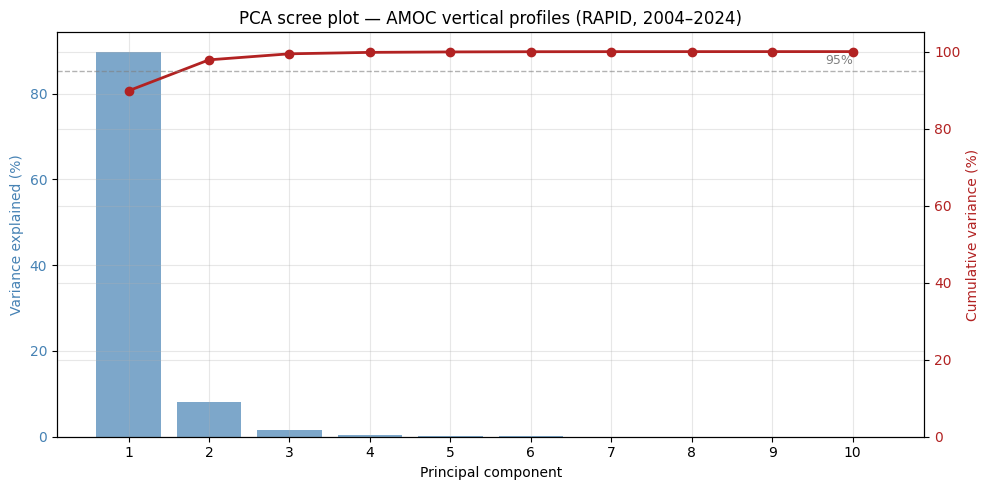
\includegraphics[width=0.8\textwidth]{figures/data_pipeline/pca_scree.png}
    \caption[Varianza spiegata dai modi PCA verticali.]{\textbf{La variabilità
    verticale dell'AMOC è quasi monodimensionale.} Varianza spiegata da ciascuna
    componente principale dei profili verticali a 307 livelli. Il primo modo da solo
    spiega il \SI{89.82}{\percent} e i primi due insieme il \SI{97.86}{\percent};
    il netto gomito dopo il secondo modo segna dove la struttura cede al rumore.
    Questo è lo spazio latente a due coordinate su cui è costruita la rappresentazione
    esperienziale.}
    \label{fig:pca-scree}
\end{figure}


Entrambi i modi hanno un chiaro significato fisico. PC1 ha lo stesso segno a ogni profondità e culmina intorno ai 1150~m, vicino a dove culmina il profilo medio (\S\ref{subsec:scene-column}): quando sale l'intera cella di rovesciamento si rafforza mantenendo la sua forma, quando scende la cella si indebolisce nel suo insieme. PC1 è l'\emph{intensità} della circolazione --- vicino al novanta per cento di ciò che l'AMOC fa da un giorno all'altro. PC2 cambia segno una volta scendendo lungo la colonna d'acqua, rafforzando la cella a una profondità mentre la indebolisce a un'altra: la \emph{ridistribuzione verticale} della circolazione, uno spostamento minore ma genuino della sua forma attorno alla media.

% it/figures/data_pipeline/mode_shapes.tex — versione italiana
\begin{figure}[!ht]
    \centering
    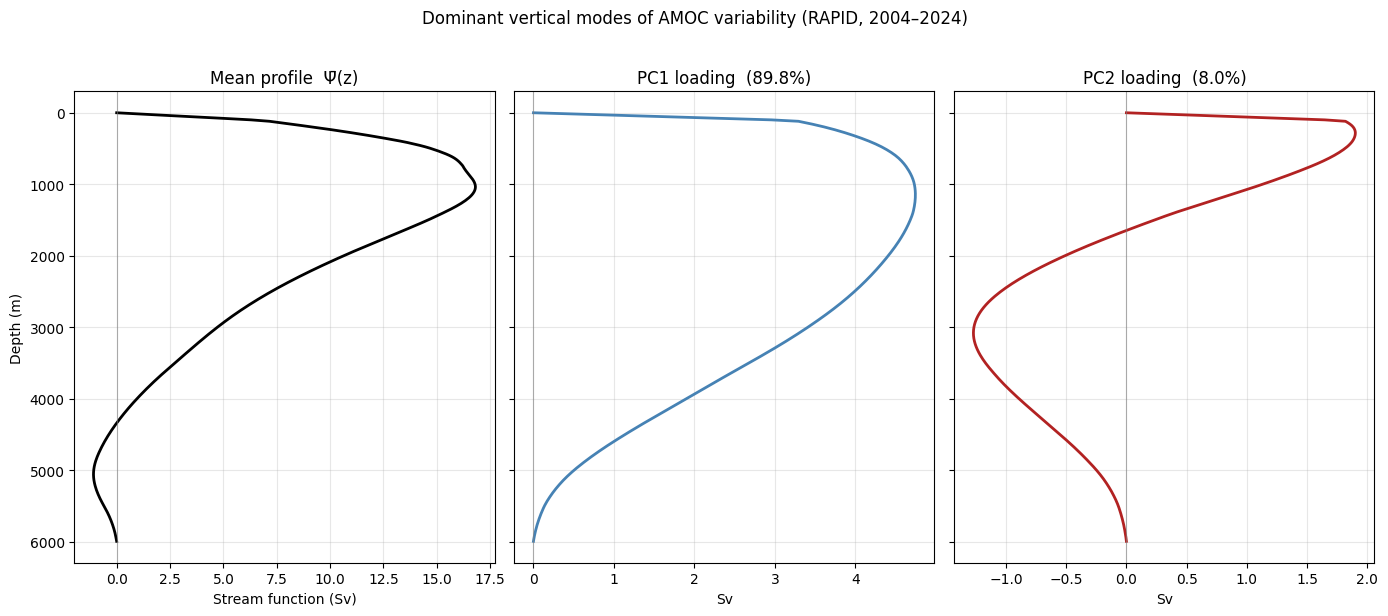
\includegraphics[width=1\textwidth]{figures/data_pipeline/mode_shapes.png}
    \caption[I due modi verticali: intensità e ridistribuzione.]{\textbf{I due
    modi che spiegano l'anatomia verticale dell'AMOC.} Ogni curva è un profilo di
    loading tracciato rispetto alla profondità. La PC1 (intensità) è un \emph{monopolo}:
    lo stesso segno a ogni profondità, con picco attorno a 1150~m, vicino alla profondità
    a cui il profilo medio ha il suo picco, così che un cambiamento nel suo score rafforza
    o indebolisce coerentemente l'intera cella di rovesciamento.
    La PC2 (ridistribuzione) è un \emph{dipolo}: cambia segno una volta con la profondità,
    rafforzando la cella a un livello mentre la indebolisce a un altro. I loading sono
    scalati in Sv per la visualizzazione. Insieme queste due forme portano il
    \SI{97.86}{\percent} della variabilità verticale.}
    \label{fig:mode-shapes}
\end{figure}


È qui che l'analisi tocca per la prima volta direttamente la tesi. Sarebbe facile assegnare significati a questi modi a posteriori; non è ciò che accade qui. Il modo di intensità è recuperato dai dati e poi confermato rispetto a un evento noto, che è una posizione più solida da cui argomentare. Seguito nel tempo, PC1 cala bruscamente durante il 2009--2010 --- l'indebolimento più accuratamente documentato del record osservativo --- raggiungendo un punteggio medio di periodo di PC1 di $-23.97$ rispetto a una media sull'intero record pari a zero.\footnote{Lo stesso evento del 2009--2010 compare indipendentemente nel campo grezzo profondità--tempo, in questa serie di intensità, e più avanti nel rilevatore di anomalie: tre metodi, un episodio fisico.} Che una singola linea possa ancora portare un evento visto per la prima volta nell'intero campo profondità--tempo è una prova piccola ma reale dell'affermazione della tesi --- che questo sistema può essere ri-rappresentato in meno dimensioni senza perdere ciò che conta. Il piano PC1--PC2, che tiene il \SI{97.86}{\percent} dell'anatomia verticale in sole due coordinate, è lo spazio latente lungo cui i profili respireranno fedelmente nel tempo nella condizione esperienziale del Capitolo~\ref{ch:translate}.

% -------------------------------------------------------------------------
\section{Una geometria della varietà essenzialmente piatta}
\label{sec:detect-ae}

Poiché la PCA è un metodo lineare, una domanda importante è se una rappresentazione lineare sia sufficiente a catturare la struttura dei dati dell'AMOC: se la geometria sottostante fosse fortemente non lineare, una proiezione lineare potrebbe semplificarla eccessivamente e perdere informazione. Il confronto che segue è interpretabile grazie a un risultato noto: un autoencoder con attivazioni lineari recupera lo stesso sottospazio della PCA, perciò qualsiasi vantaggio che un autoencoder non lineare mostri a dimensionalità pari è attribuibile alla curvatura della varietà dei dati \citep{baldi1989}. Uno scarto quasi nullo è quindi evidenza di piattezza, non meramente di un pareggio. Il secondo obiettivo (O1.2) testa quindi questa assunzione confrontando la PCA con un autoencoder non lineare addestrato sugli stessi 14{,}596 profili AMOC. Entrambi i modelli sono valutati usando lo stesso numero di dimensioni latenti. Se la struttura latente fosse genuinamente non lineare, ci si aspetterebbe che l'autoencoder ricostruisca i dati più accuratamente. In caso contrario, la PCA dovrebbe comportarsi altrettanto bene.

I risultati sostengono chiaramente la seconda ipotesi. Attraverso le dimensioni latenti da una a cinque l'autoencoder non lineare non ha mai superato la PCA, che è stata costantemente migliore di $-0.06$ a $-0.15$ punti percentuali (Tabella~\ref{tab:ae-gap}); alle due dimensioni usate ovunque, la PCA ha ricostruito il \SI{97.86}{\percent} contro il \SI{97.77}{\percent} dell'autoencoder.\footnote{I livelli di superficie e di fondale sono stati esclusi dall'input dell'autoencoder perché la funzione di corrente è fissata a zero a entrambi i confini per conservazione della massa e quindi non contiene varianza apprendibile.} Questo conferma H2: pur libero di apprendere trasformazioni non lineari, l'autoencoder non ha trovato alcuna struttura significativa oltre la rappresentazione lineare PCA.

% it/figures/data_pipeline/tab_ae_gap.tex — versione italiana
\begin{table}[!ht]
    \centering
    \small
    \caption[Autoencoder contro PCA a dimensione latente appaiata.]{Ricostruzione
    dei profili verticali da parte di un autoencoder non lineare contro la PCA lineare,
    a dimensione latente $k$ appaiata. Lo scarto è negativo a ogni $k$: la PCA non è mai
    battuta, quindi la varietà è piatta. Gli scarti sono calcolati da valori non
    arrotondati, perciò possono differire di 0.01 dalla differenza delle colonne
    arrotondate.}
    \label{tab:ae-gap}
    \begin{tabular}{@{}crrr@{}}
        \toprule
        \textbf{$k$} & \textbf{PCA cum.\ \%} & \textbf{AE $R^2_{\mathrm{Sv}}$ \%} & \textbf{Scarto (pp)} \\
        \midrule
        1 & 89.82 & 89.67 & $-0.15$ \\
        2 & 97.86 & 97.77 & $-0.08$ \\
        3 & 99.42 & 99.36 & $-0.06$ \\
        4 & 99.80 & 99.74 & $-0.06$ \\
        5 & 99.91 & 99.83 & $-0.08$ \\
        \bottomrule
    \end{tabular}
\end{table}

% it/figures/data_pipeline/fig_manifold.tex — versione italiana
\begin{figure}[!ht]
    \centering
    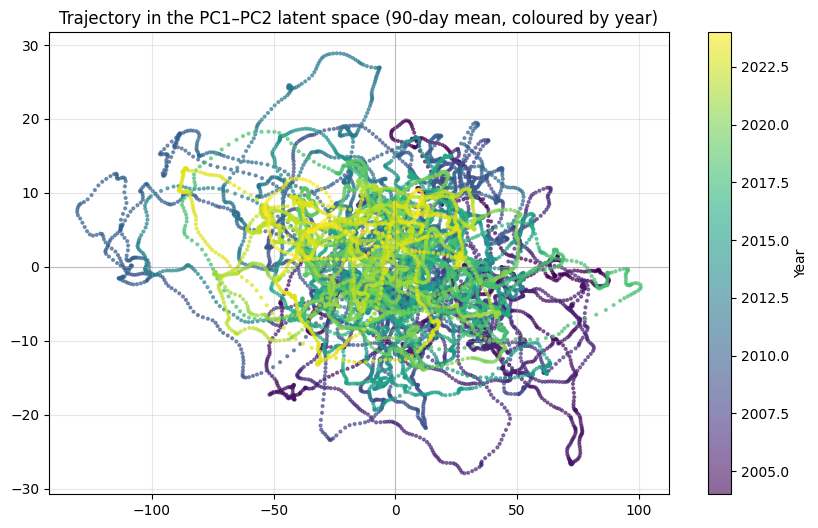
\includegraphics[width=0.85\textwidth]{figures/data_pipeline/fig_manifold.png}
    \caption[La varietà latente piatta dei profili AMOC.]{\textbf{La varietà dei
    profili verticali dell'AMOC è piatta.} Ogni punto è un profilo, collocato dalle
    sue due coordinate latenti --- PC1 (intensità) e PC2 (ridistribuzione verticale).
    Un autoencoder non lineare addestrato sugli stessi profili non li ricostruisce
    meglio della PCA lineare a nessuna dimensione latente (scarto da $-0.06$ a $-0.15$
    punti percentuali; vedi Tabella~\ref{tab:ae-gap}), confermando che due coordinate
    rettilinee catturano la struttura senza distorsione.}
    \label{fig:manifold}
\end{figure}


Questo risultato è importante perché giustifica l'uso delle coordinate latenti lungo l'intera fase di \emph{Traduzione} della tesi. Se la varietà sottostante fosse stata fortemente curva, rappresentare il sistema usando le prime due componenti principali avrebbe introdotto distorsioni forzando una struttura non lineare in uno spazio lineare. Invece, i risultati mostrano che la varietà latente è effettivamente lineare. Di conseguenza, le prime due componenti principali forniscono una rappresentazione tanto altamente interpretabile quanto altamente fedele ai dati originali. Le coordinate possono quindi essere interpretate in modo significativo come modi distinti di variabilità dell'AMOC senza sacrificare l'accuratezza di rappresentazione. In questo caso, l'interpretabilità arriva praticamente a costo nullo in fedeltà, rendendo la rappresentazione proposta tanto scientificamente difendibile quanto adatta come base per le visualizzazioni esperienziali sviluppate nel capitolo seguente.

% -------------------------------------------------------------------------
\section{Segnali di preallarme e risultato nullo}
\label{sec:detect-ews}

Il terzo obiettivo (O1.3) chiede se il record contenga segnali di preallarme di un punto di tipping in avvicinamento. Per la teoria del rallentamento critico, un sistema che si avvicina a una biforcazione mostra varianza crescente e autocorrelazione a lag-1 \citep{dakos2012, scheffer2009}. Testare ciò richiede particolare cura, e qui l'analisi mette in luce un importante problema metodologico.

A prima vista i risultati appaiono molto forti. La varianza mobile della serie di intensità tende al rialzo, con $\tau$ di Kendall $= +0.078$ e un p-value di $2\times10^{-42}$; anche l'autocorrelazione mobile aumenta, con $\tau = +0.088$ e un p-value di $1\times10^{-52}$. Presi alla lettera sarebbero un segnale estremamente forte. L'interpretazione è fuorviante, perché le finestre mobili si sovrappongono sostanzialmente e le migliaia di valori calcolati non sono osservazioni indipendenti.\footnote{Il test di Kendall assume indipendenza. Qui le statistiche mobili usano finestre di 730 profili (un anno) fortemente sovrapposte, perciò i valori consecutivi sono altamente dipendenti --- effetto amplificato dalla forte autocorrelazione della serie originale ($0.943$). Il software restituisce un p-value molto piccolo senza tenere conto di quella dipendenza, facendo apparire il risultato più certo di quanto sia.} Quando si usa invece il numero effettivo di osservazioni indipendenti --- circa 19,5 finestre non sovrapposte di 730 profili --- e il test è corretto di conseguenza, le tendenze apparenti scompaiono. Il p-value corretto per la tendenza della varianza è \textbf{0.634}, mentre per la tendenza dell'autocorrelazione è \textbf{0.595}. Nessuno dei due risultati è statisticamente significativo (Tabella~\ref{tab:ews}). Il forte segnale iniziale era quindi causato dal trattare osservazioni dipendenti come se fossero indipendenti.

% it/figures/data_pipeline/tab_ews.tex — versione italiana
\begin{table}[!ht]
    \centering
    \small
    \caption[Trend di preallarme: significatività ingenua contro corretta.]{Test di
    trend con il $\tau$ di Kendall per i due segnali classici di preallarme. I p-value
    ingenui trattano le finestre sovrapposte come indipendenti; i p-value corretti
    contano le $\sim$19.5 finestre indipendenti che il record contiene. Nessuno dei due
    trend è significativo.}
    \label{tab:ews}
    \begin{tabular}{@{}lcccc@{}}
        \toprule
        \textbf{Segnale} & \textbf{Kendall $\tau$} & \textbf{p ingenuo} & \textbf{p corretto} & \textbf{Verdetto} \\
        \midrule
        Varianza mobile & $+0.078$ & $2\times10^{-42}$ & 0.634 & non significativo \\
        AR(1) mobile     & $+0.088$ & $1\times10^{-52}$ & 0.595 & non significativo \\
        \bottomrule
    \end{tabular}
\end{table}

% it/figures/data_pipeline/fig_ews.tex — versione italiana
\begin{figure}[!ht]
    \centering
    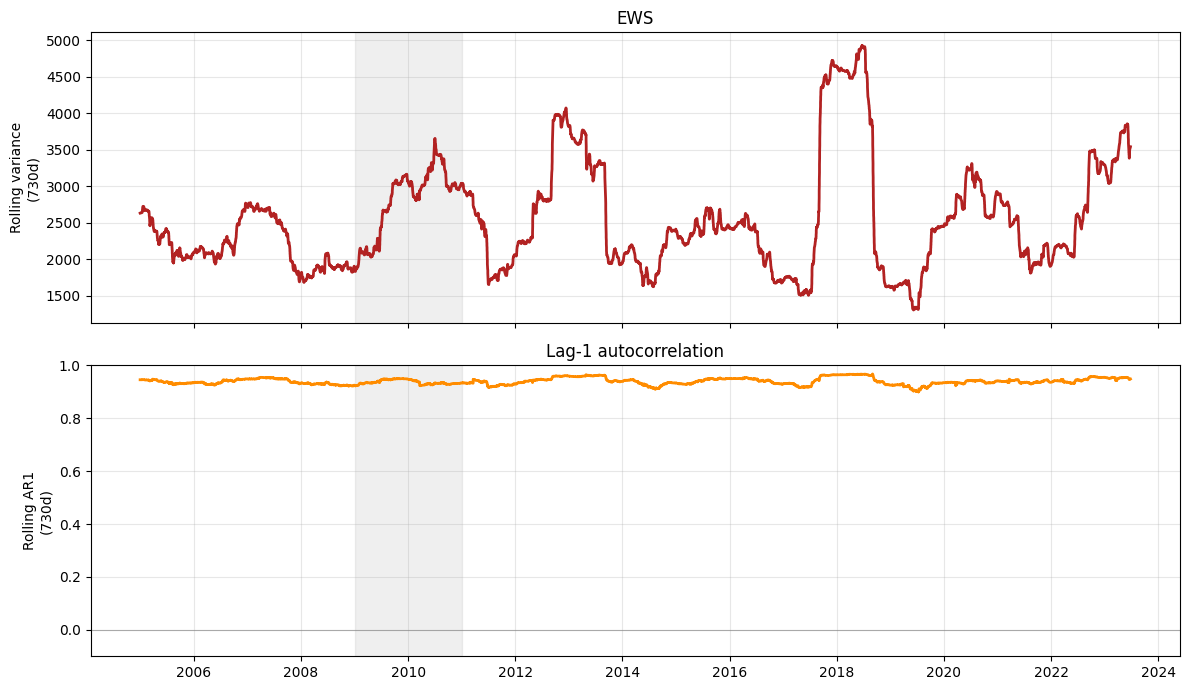
\includegraphics[width=0.9\textwidth]{figures/data_pipeline/ews.png}
    \caption[Segnali di preallarme: varianza mobile e autocorrelazione.]{\textbf{Nessun
    trend di preallarme rigoroso.} Varianza mobile e autocorrelazione a lag~1 della serie
    di intensità lungo il record. Entrambe oscillano senza una salita sostenuta.
    I loro p-value di trend ingenui ($\sim$$10^{-42}$) sono artefatti di finestre
    fortemente sovrapposte; corretti per le $\sim$19.5 finestre indipendenti che il
    record contiene davvero, i trend non sono significativi (p~$=$~0.634 e
    0.595; Tabella~\ref{tab:ews}).}
    \label{fig:ews}
\end{figure}


La conclusione finale è quindi un \emph{risultato nullo}. Una volta considerata correttamente la struttura di dipendenza dei dati, gli indicatori classici di preallarme non possono essere distinti dal rumore. Questo sostiene H3 nella sua forma nulla e rappresenta un importante contributo metodologico anziché un limite. Un risultato positivo ottenuto interpretando male le statistiche sarebbe stato più attraente, ma non sarebbe stato affidabile. Dimostrare che un segnale apparentemente forte scompare una volta affrontata la dipendenza statistica è il risultato sostanziale qui. Indipendentemente da quella correzione, il record è semplicemente troppo breve per la domanda: vent'anni dell'array RAPID sono assai più brevi della scala temporale da multidecennale a centennale su cui si svilupperebbe un tipping dell'AMOC, perciò l'assenza di una tendenza di preallarme qui dice ciò che questo record può sostenere, non se l'AMOC si stia avvicinando a una soglia. Per le stesse ragioni gli indicatori sono calcolati sulla serie di intensità grezza, senza detrending. Rimuovere prima una tendenza lenta è standard nel lavoro sul rallentamento critico, così che varianza e autocorrelazione riflettano le fluttuazioni anziché la tendenza stessa; qui non si fa perché in vent'anni non c'è alcuna tendenza robusta da rimuovere --- i test corretti sono essi stessi non significativi --- e una finestra di detrending è una scelta arbitraria che può fabbricare o cancellare un segnale apparente. Lasciare grezza la serie mantiene il risultato nullo poggiante sulla sola correzione per la dipendenza, al costo che ogni tendenza residua, e il ciclo stagionale mantenuto, restano nella varianza che gli indicatori misurano. Il confine tra rilevamento di pattern e predizione che questa fase osserva è registrato nell'Appendice~\ref{app:limits-detect}.

% -------------------------------------------------------------------------
\section{Rilevamento di anomalie}
\label{sec:detect-anomalies}

L'analisi di preallarme cerca lente \emph{tendenze}; una domanda diversa riguarda singoli \emph{eventi} --- quali momenti si discostano dal comportamento normale. Un Isolation Forest sulle coordinate PC1--PC2 segnala il \SI{5}{\percent} del record (730 profili) come anomalo, concentrato nel 2009--2010 (158 profili), 2012--2013 (100 profili) e 2018 (66 profili). Il punteggio di anomalia non aumenta nel tempo: i momenti insoliti sono distribuiti lungo il record anziché accumularsi verso la fine, un'altra indicazione che il sistema non si sta muovendo progressivamente verso una soglia.

% it/figures/data_pipeline/fig_anomalies.tex — versione italiana
\begin{figure}[!ht]
    \centering
    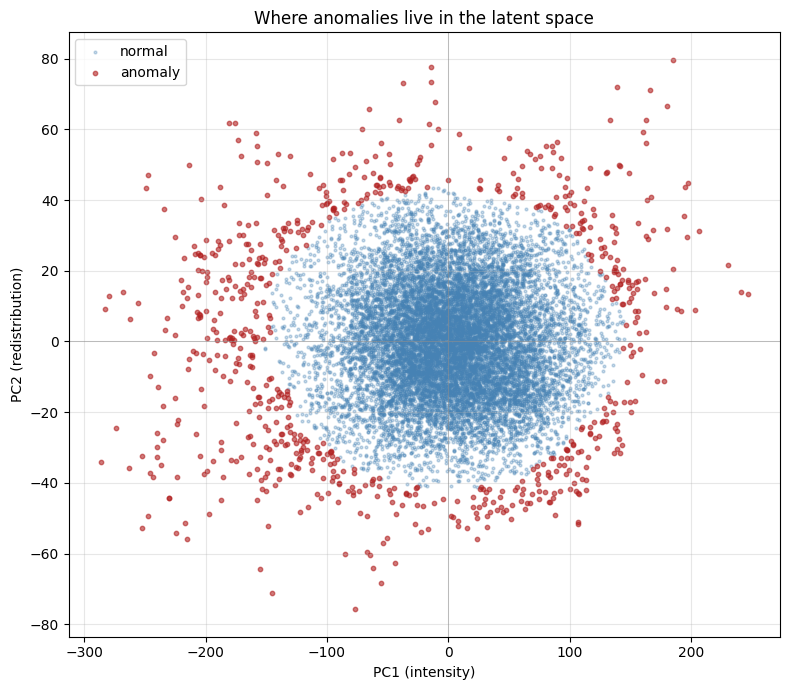
\includegraphics[width=0.9\textwidth]{figures/data_pipeline/anomalies.png}
    \caption[Anomalie Isolation Forest lungo il record.]{\textbf{Eventi anomali
    discreti, distribuiti lungo il record.} L'Isolation Forest segnala il
    \SI{5}{\percent} dei profili (730) come anomali nel piano PC1--PC2. Si addensano
    nel 2009--2010 (158 profili), nel 2012--2013 (100) e nel 2018 (66), senza trend nel
    tempo --- a conferma del risultato nullo di preallarme da un metodo diverso. Questi
    momenti diventano texture percepibile (principio di grammatica~P3) nel
    Capitolo~\ref{ch:translate}.}
    \label{fig:anomalies}
\end{figure}


Due aspetti sono importanti per questa tesi. Primo, questa analisi sostiene il risultato nullo da una prospettiva completamente indipendente: un algoritmo che non si basa sulla teoria del preallarme non trova anch'esso alcuno spostamento graduale, ma piuttosto eventi isolati distribuiti lungo il record ventennale. Raggiunge la stessa conclusione con un metodo diverso.\footnote{I cluster di anomalie corrispondono a caratteristiche identificate indipendentemente --- l'indebolimento del 2009--2010 e i picchi di varianza del 2012--2013 e del 2018 --- con il \SI{41.4}{\percent} dei profili anomali che ricade nel quarto più alto di varianza locale. Metodi diversi rivelano lo stesso comportamento fisico.} Secondo, queste anomalie forniscono la base per una specifica decisione di design. Seguendo la grammatica introdotta nel Capitolo~\ref{ch:literature}, gli scostamenti dal regime normale possono essere tradotti in cambiamenti locali di texture percettiva (principio~P3). I momenti identificati dal rilevatore sono quindi gli stessi momenti che la rappresentazione esperienziale trasformerà in cambiamenti percepibili --- il che significa che il rilevamento di anomalie non è solo un risultato sull'AMOC, ma anche un input diretto per come l'AMOC è rappresentata.

% -------------------------------------------------------------------------
\section{Osservazione a confronto con la rianalisi}
\label{sec:detect-copernicus}

Il passo finale confronta le osservazioni RAPID con l'ensemble di rianalisi Copernicus GREP sui 237 mesi che condividono, per caratterizzare quanto bene la rianalisi riproduca il segnale osservato e per identificare l'incertezza che la fase di \emph{traduzione} deve comunicare. L'accordo è moderato: correlazione 0,754, un piccolo bias di $+0.584$~Sv con RAPID leggermente più forte, e una differenza quadratica media di 2,300~Sv. Entrambi restano vicini ai 17~Sv e variano in modo simile nel tempo, perciò la rianalisi cattura il comportamento complessivo della circolazione anche dove sbaglia singoli mesi.

Il risultato più informativo riguarda la copertura dell'incertezza. RAPID ricade entro l'intervallo di $\pm1$ deviazione standard dell'ensemble di rianalisi solo nel \SI{40.1}{\percent} dei mesi.\footnote{Se la dispersione dell'ensemble rappresentasse una stima ben calibrata della propria incertezza, l'osservazione dovrebbe ricadere entro l'intervallo di una deviazione standard molto più spesso. Una copertura più bassa indica che la dispersione è troppo stretta rispetto agli errori effettivi.} Un ensemble di modelli con un intervallo di incertezza realistico dovrebbe catturare l'osservazione più frequentemente. Questa bassa copertura indica che l'ensemble è \emph{troppo sicuro di sé}: l'incertezza che riporta è minore dell'errore reale. Questo punto è importante per la tesi perché la dispersione dell'ensemble è esattamente ciò che la fase di \emph{traduzione} converte in incertezza percepibile, secondo il principio~P4 della grammatica di design. Comprendere che questa incertezza è sottostimata è quindi parte del rappresentarla onestamente: la visualizzazione può comunicare l'incertezza del modello chiarendo al contempo che l'incertezza reale è probabilmente maggiore.

% -------------------------------------------------------------------------
\section{Sintesi analitica}
\label{sec:detect-summary}

La fase analitica consegna alla fase di \emph{traduzione} un substrato documentato anziché assunto. Due coordinate interpretabili --- intensità e ridistribuzione verticale --- portano il \SI{97.86}{\percent} della variabilità verticale dell'AMOC, e un modello non lineare conferma che la varietà è abbastanza piatta da usarle senza distorsione rilevante. Il record non mostra alcuna tendenza robusta di preallarme ma contiene anomalie discrete che possono diventare texture percettiva, e il confronto con la rianalisi fornisce una stima dell'incertezza fisicamente significativa, benché troppo stretta. Ciascuno è un input giustificato per un substrato compatto, fedele, interpretabile, consapevole degli eventi e portatore di incertezza, su cui un sistema invisibile può essere reso percepibile senza essere travisato.


\setpartsubtitle{Dalla struttura latente alla rappresentazione esperienziale}
\part{TRADURRE}
% =========================================================================
% CAPITOLO 7 — TRADURRE: PROGETTARE RAPPRESENTAZIONI ESPERIENZIALI
% =========================================================================

\chapter{Progettare rappresentazioni esperienziali}
\label{ch:translate}

\noindent
{\rmfamily\itshape
\begin{tabular}[t]{@{}l@{\hspace{0.3cm}}p{12.5cm}@{}}
\textls[50]{\textbf{Trattati:}} &
\textls[50]{Prototipo e Minimum Viable Product · Equivalenza informativa · Fedeltà e
provenienza · Grammatica di design · Mappatura percettiva · Tre scene · Sonificazione}
\end{tabular}
}

\vspace{0.5cm}

Il Capitolo~\ref{ch:data_pipeline} ha stabilito che cosa c'è da rappresentare. Questo capitolo stabilisce come è rappresentato, e perché quelle scelte sono difendibili. Documenta i tre artefatti del progetto \emph{Living Atlantic}, il framework che governa tutti e tre, e la grammatica di design offerta come contributo trasferibile di questa tesi sotto l'obiettivo~O2.2.

% -------------------------------------------------------------------------
\section{Dalla struttura latente alla forma percettiva}
\label{sec:translate-premise}

Il Capitolo~\ref{ch:data_pipeline} ha stabilito che due modi lineari spiegano il $97.86\%$ della varianza nei profili verticali dell'AMOC, e che un autoencoder non lineare non supera mai la decomposizione lineare a dimensionalità pari (O1.2). La varietà su cui vive il record osservativo è essenzialmente piatta, e questo fatto autorizza tutto in questo capitolo: se fosse stata curva, muoversi attraverso il piano recuperato dalla PCA passerebbe per stati che l'oceano non ha mai occupato. Poiché è piatta, ogni mese è un punto, e animare lungo il percorso tra i mesi mostra stati sul piano che il record occupa.\footnote{Per il risultato di Baldi--Hornik, ogni guadagno dell'autoencoder sulla PCA è attribuibile alla sola curvatura; lo scarto quasi nullo conferma che la varietà è abbastanza piatta perché coordinate lineari la sostituiscano fedelmente \parencite{baldi1989}.} L'ipotesi~H2 non è quindi un risultato negativo ma il fondamento della fase di rappresentazione. Senza di essa, il livello esperienziale non avrebbe alcun terreno epistemico.

È anche questo il senso in cui qui il machine learning opera in modo rappresentativo anziché predittivo. I modelli del Capitolo~\ref{ch:data_pipeline} non fanno previsioni; propongono un sistema di coordinate. Seguendo \textcite{iten2020}, esteso all'esplorazione interattiva da \textcite{camps2019}, la rappresentazione latente è trattata come un oggetto che un interprete umano può esaminare e abitare. Ciò che questo capitolo aggiunge è rendere lo spazio latente percepibile a un osservatore che non sa che esiste \parencite{sacha2018}.

% -------------------------------------------------------------------------
\section{Il framework di traduzione}
\label{sec:translate-framework}

Quattro impegni e uno strumento governano tutte e tre le scene, enunciati una volta qui e applicati più sotto.

\subsection{Equivalenza informativa per provenienza condivisa}
\label{subsec:equivalence}

L'obiettivo~O2.1 richiede che le due condizioni --- statica convenzionale (C1) e dinamica-esperienziale (C2+C3) --- attingano agli stessi dati attraverso la stessa ricostruzione, allineate per provenienza, inquadramento e unità di misura. Non sono deliberatamente allineate nel contenuto informativo: la condizione esperienziale espone la dimensione temporale che quella statica trattiene, che è esattamente la variabile che lo studio esamina. Una differenza osservata nella valutazione è quindi attribuibile alla forma e a quell'unica aggiunta intenzionale, non a contenuto extra arbitrario. \textcite{tversky2002} ha mostrato perché questa non è una formalità: l'apparente superiorità dei grafici animati si dissolve ovunque la condizione animata porti informazione che quella statica non ha.\footnote{Una versione precedente del progetto imponeva questa equivalenza attraverso un'architettura a documenti condivisi. Benché lo studio sia stato poi ridisegnato come esperimento tra soggetti, lo stesso principio rimane: entrambe le condizioni sono generate dallo stesso bundle di dati e dalla stessa pipeline di ricostruzione, differendo solo nelle scelte di rappresentazione applicate.}

Lo studio finale adotta un disegno tra soggetti: ogni partecipante è assegnato a una singola condizione ed esperisce tutte e tre le scene entro quella condizione.\footnote{I file somministrati sono \texttt{column-static.html}, \texttt{theengine-static.html} e \texttt{thethreshold-static.html} (C1), e le loro controparti \texttt{-experiential} (C2+C3). Un terzo file per scena espone tutte le condizioni dietro un interruttore per dimostrazione e non è somministrato.} Questo rimuove gli effetti di trascinamento che un disegno sequenziale introdurrebbe, al costo del confronto intra-persona --- uno scambio appropriato per un disegno esplorativo analizzato rispetto a una griglia fissata prima di leggere le risposte \parencite{braunclarke2019}.

L'equivalenza è quindi garantita non dalla struttura dei file ma da una pipeline di provenienza condivisa: entrambe le condizioni sono generate dallo stesso bundle di dati, ricostruiscono ogni profilo attraverso la stessa funzione, e documentano ogni elemento percepibile in un registro di provenienza comune.\footnote{\texttt{amoc\_translate\_bundle.json} (schema v1.0.0), \texttt{shared/reconstruct.js} e \texttt{shared/bundle.js} rispettivamente; il registro è la Tabella~\ref{tab:ledger} nell'Appendice~\ref{app:code}, che documenta anche l'architettura dei moduli e la struttura del repository.}

\subsection{Fedeltà}
\label{subsec:fidelity}

Ogni valore a schermo deriva dal bundle. Nulla è ridimensionato per effetto visivo, e dove una preferenza estetica confliggeva con i dati, hanno vinto i dati.\footnote{I punti in cui questo è costato qualcosa sono registrati nell'Appendice~\ref{app:limits-translate}.} La ricostruzione è un'unica equazione, condivisa da ogni scena e da entrambe le condizioni:

\begin{equation}
\label{eq:reconstruction}
\Psi(z, t) = \overline{\Psi}(z) + \mathrm{pc}_1(t) \cdot B_1(z) + \mathrm{pc}_2(t) \cdot B_2(z)
\end{equation}

dove $\overline{\Psi}$ è la media del record, $B_1$ e $B_2$ sono i vettori di base unitari della decomposizione e $\mathrm{pc}_1$, $\mathrm{pc}_2$ le coordinate latenti del mese~$t$.\footnote{Il bundle porta anche i loading EOF --- gli stessi modi scalati in Sverdrup solo per la visualizzazione della forma del modo. Non devono mai essere passati all'Equazione~\ref{eq:reconstruction}; vedi Appendice~\ref{app:code}.}

L'equivalenza può essere verificata rispetto a questa equazione: la condizione statica valuta la ricostruzione condivisa con entrambi i coefficienti posti a zero, restituendo esattamente il profilo medio memorizzato. C1 segue quindi lo stesso percorso computazionale della condizione sperimentale mostrando solo dati osservati; il modello entra quando la curva comincia a muoversi.

\subsection{Il machine learning come substrato}
\label{subsec:ml-role}

Il contributo del machine learning è strutturale, non generativo. La velocità meridionale locale che guida il campo di particelle è la derivata verticale della funzione di corrente:

\begin{equation}
\label{eq:velocity}
v(z, t) \propto \frac{\partial \Psi(z, t)}{\partial z}
\end{equation}

\noindent È su questa distinzione che ruota l'errore sulla funzione di corrente della \S\ref{sec:res-misconception}: l'\emph{altezza} della curva è trasporto cumulato, la sua \emph{pendenza} è flusso locale. Il modello non disegna la curva del profilo, non colora le particelle e non produce lo stato medio; il registro li annota come classici.\footnote{Il campo di particelle è una derivata di $\Psi$ (Equazione~\ref{eq:velocity}) che qualsiasi analista potrebbe riprodurre con un operatore di differenza. Il modello tocca solo il sistema di coordinate e i punteggi di anomalia.} Ciò che il modello fornisce è il sistema di coordinate latenti lungo cui il profilo si muove nel tempo, e i momenti che se ne discostano. L'originalità non è un nuovo algoritmo ma un ponte empirico: uno spazio latente appreso usato come substrato su cui un sistema complesso è reso percepibile a un non esperto, con il ruolo del modello confinato a dove i dati lo autorizzano e dichiarato elemento per elemento (Tabella~\ref{tab:ledger}).

\subsection{La grammatica di design}
\label{subsec:grammar}

L'obiettivo~O2.2 chiede una grammatica di design che mappi le feature derivate dal machine learning su dimensioni percettive, fondata sull'elaborazione pre-attentiva della \S\ref{sec:empirical-viz} e sulla cognizione incarnata della \S\ref{sec:embodied-viz}, e riutilizzabile oltre questo caso. È enunciata nella Tabella~\ref{tab:design-grammar} e non ripetuta qui.\footnote{I suoi sei principi, in breve: P0, l'informazione più importante al canale più accurato \parencite{munzner2014,bertin1983}; P1, entità ordinata alla posizione spaziale \parencite{clevelandmcgill1984}; P2, dinamiche al movimento reale \parencite{sterman2008,cronin2009}; P3, anomalia a densità e texture \parencite{bertin1983,ware2021}; P4, incertezza a variabilità animata; P5, variabile ordinata secondaria al suono \parencite{hermann2011}.} Ogni scena registra quali principi realizza, così che una mappatura che fallisce in valutazione ricada su quella mappatura --- e attraverso di essa sul principio --- anziché sull'artefatto nel suo insieme.

\subsection{Simmetria dell'inquadramento}
\label{subsec:symmetry}

Entro ciascuna scena, entrambe le condizioni importano gli stessi moduli di inquadramento in modo identico byte per byte: un'introduzione che porta la domanda guida della scena, e un pannello di contesto che dà la fonte dei dati e un resoconto in linguaggio piano di ciò che si misura.\footnote{\texttt{shared/intro-*.js} e \texttt{shared/context-*.js}, una coppia per scena. L'identità è per importazione anziché per duplicazione, così che i due documenti non possano divergere per una modifica a uno di essi.} A entrambi i gruppi si può insegnare a leggere lo strumento, ma a nessuno si può dire la lettura: i partecipanti imparano cosa misura $\Psi$ e cos'è uno sverdrup, perché un osservatore che non sa leggere le unità non può articolare nulla, ma non viene mai detto loro cosa significhi la struttura. Se all'osservatore va detto, la traduzione ha fallito, e la valutazione misurerebbe il testo di inquadramento anziché la rappresentazione.

La domanda guida di ciascuna scena è ciò che rende tutto questo misurabile: posta in modo identico a entrambi i gruppi, non risposta da alcun documento, e mantenuta visibile per tutto il tempo.\footnote{Le tre domande sono riprodotte nell'Appendice~\ref{app:protocols} nella forma somministrata. Mantenere la domanda visibile anziché mostrarla una sola volta è una scelta di design: senza un compito enunciato, una rappresentazione in movimento si legge come decorazione anziché come indagine.} La simmetria non è una cortesia verso il gruppo di controllo; è ciò che dà al confronto un qualunque significato, ed è ciò che l'aspettativa~E3.1 verifica.

% -------------------------------------------------------------------------
\section{Tre scene, una discesa}
\label{sec:three-scenes}

Le tre scene sono fatte per essere esperite in ordine, e l'ordine è interpretativo anziché estetico. Segue lo schema d'immagine verticale che \citet{lakoff1999} identificano come risorsa cognitiva pre-concettuale --- verso il basso come più profondo, più nascosto, più fondamentale. Un osservatore che incontra il piano latente della Scena~II senza aver prima abitato la colonna della Scena~I non ha referente per le coordinate; chi incontra la dispersione d'ensemble della Scena~III senza aver guardato la traiettoria osservata non ha baseline rispetto a cui il disaccordo si registri. Ogni scena è la condizione di intelligibilità della successiva --- e, come la \S\ref{sec:eval-limitations} registra, un confondimento per qualsiasi confronto tra esse.

Le scene sono nondimeno documenti separati, così che il questionario presenti una scena in una condizione senza stato di interazione accumulato.\footnote{La continuità è portata dall'inquadramento scritto che precede ciascuna scena e dall'ordine di somministrazione, non da transizioni animate tra esse.} Ciascuna è descritta più sotto con gli stessi sei criteri: obiettivo, strategia di rappresentazione, mappatura, condizioni, fedeltà e contributo atteso. La Tabella~\ref{tab:scene-summary} riassume le tre a colpo d'occhio.

\subsection{Scena I: La colonna}
\label{subsec:scene-column}

\begin{quote}
\textbf{Domanda guida.} \emph{L'acqua si muove tutta allo stesso modo? Se no --- come, e in quali direzioni, si muove?}
\end{quote}

\begin{figure}[htbp]
  \centering

  \begin{subfigure}[t]{0.48\textwidth}
    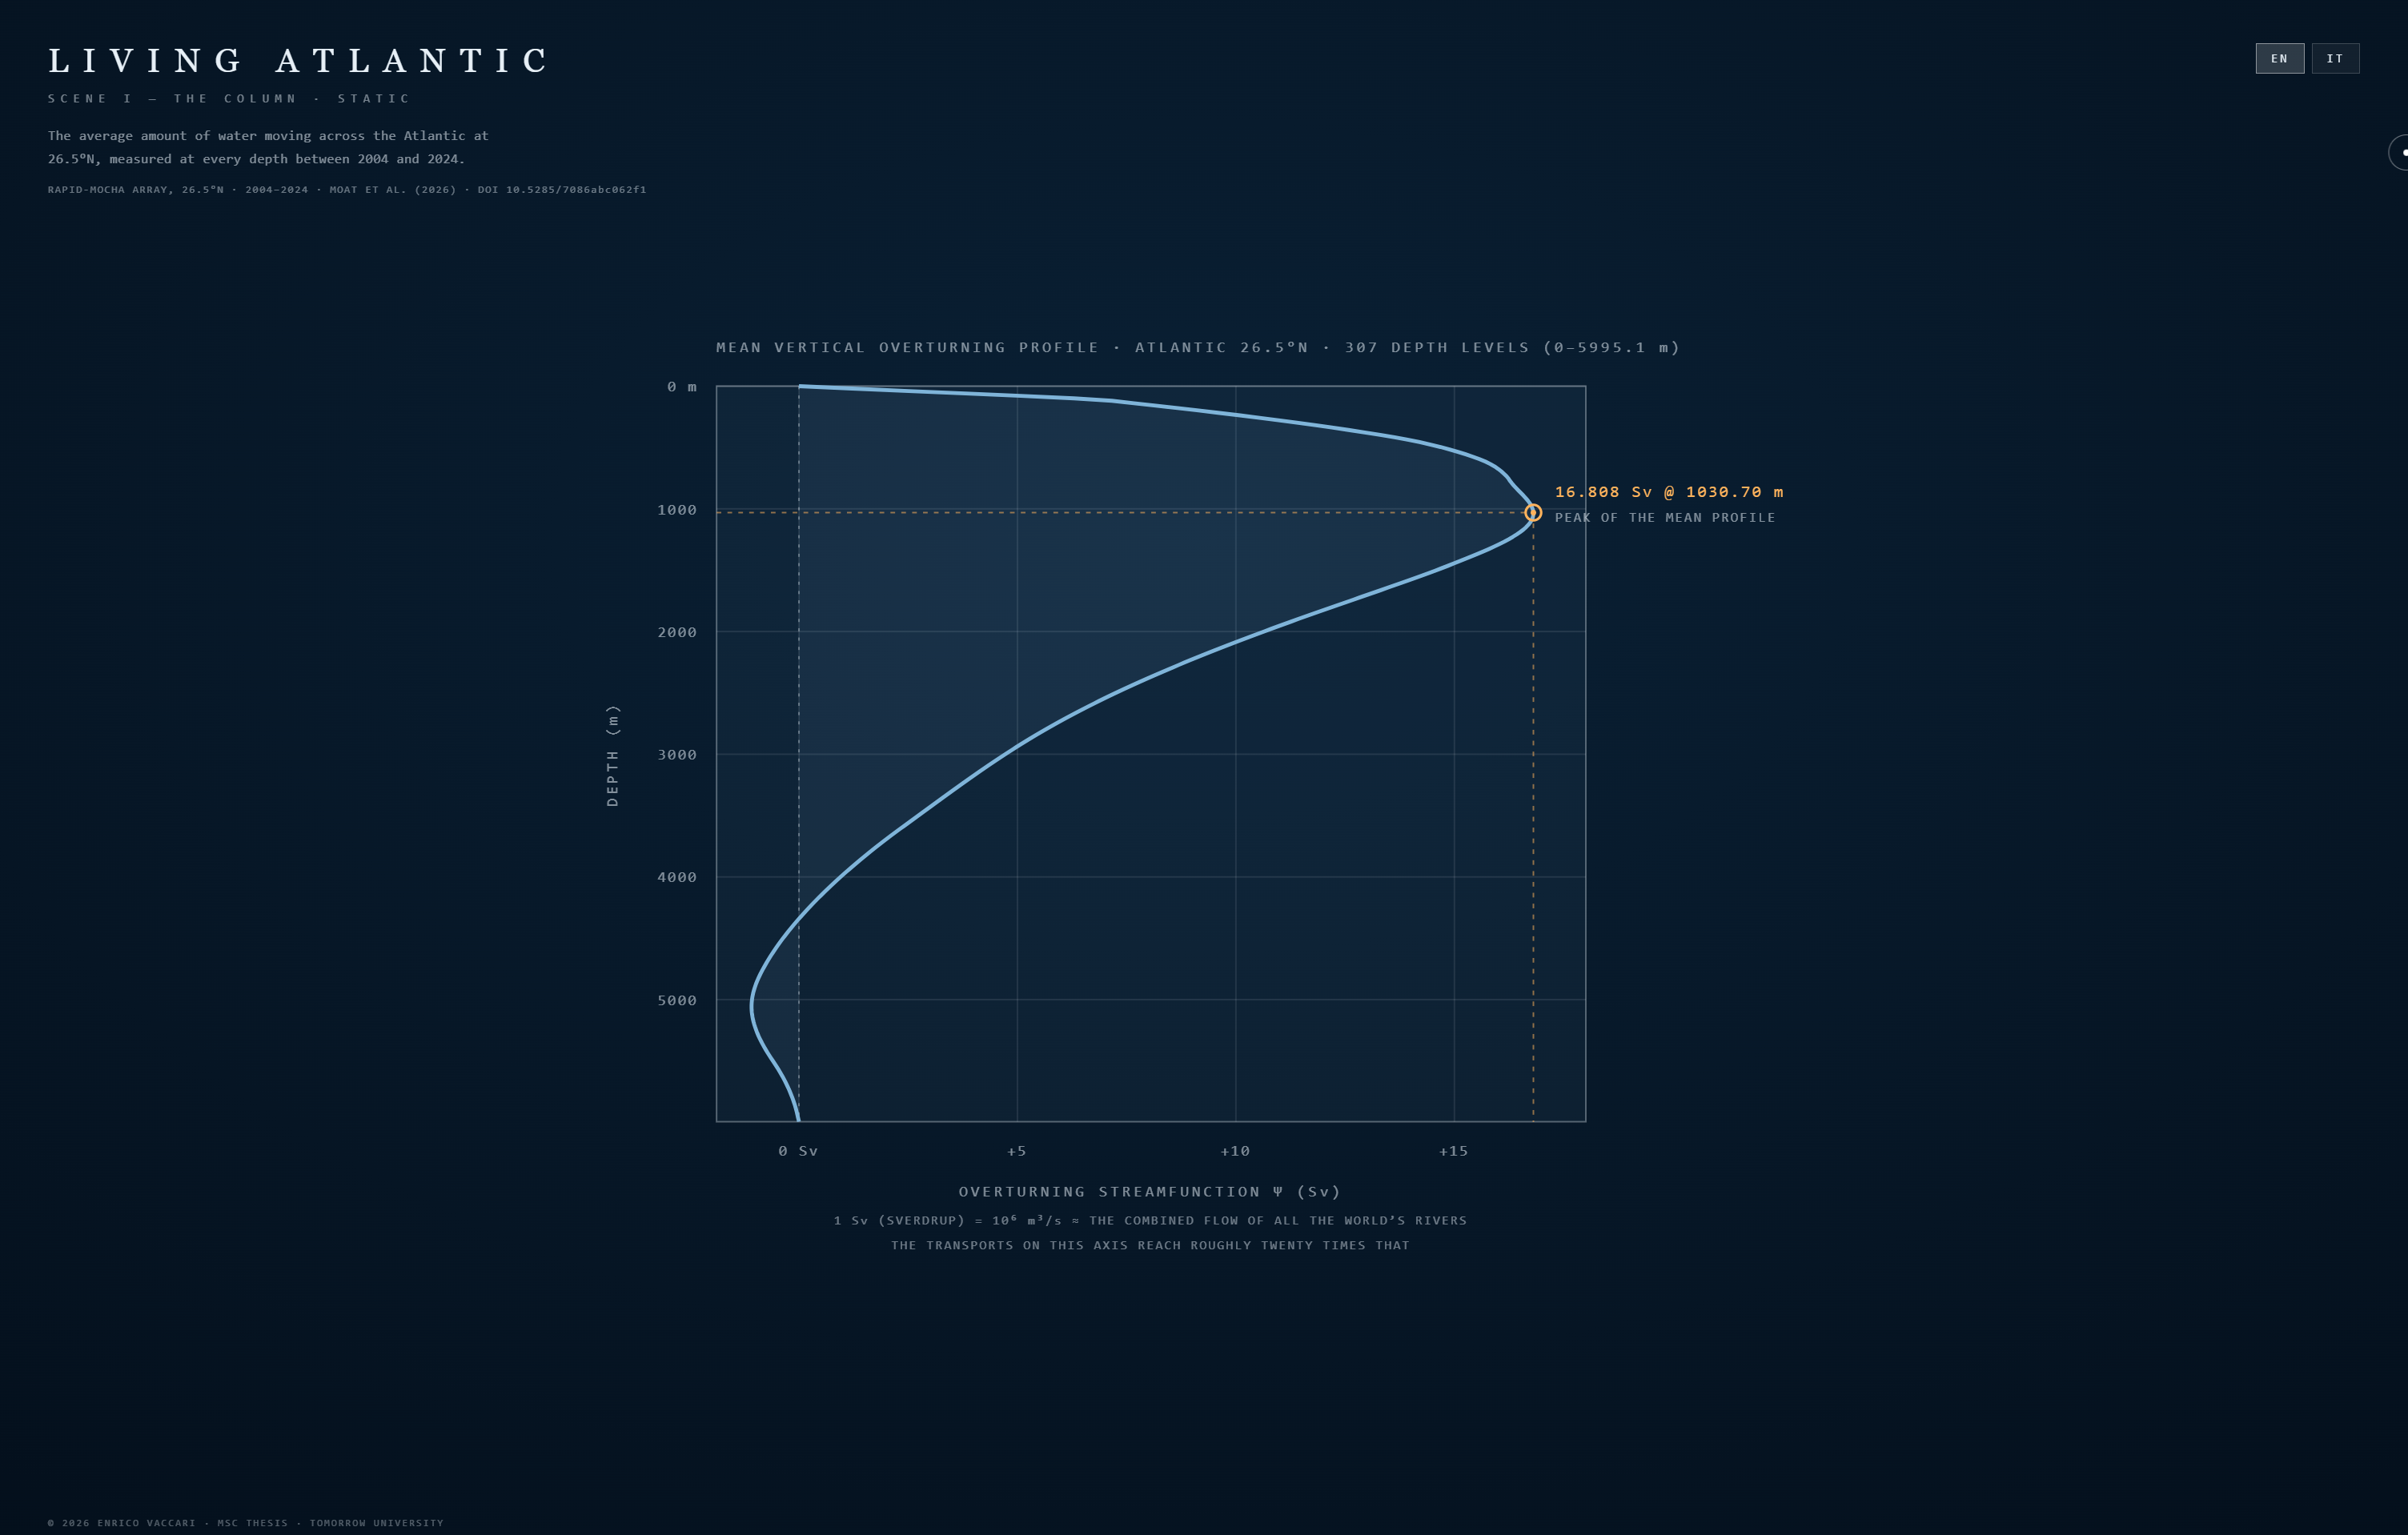
\includegraphics[width=\textwidth]{figures/viz1/viz1_column-static.png}
    \caption{Control (C1): the canonical static profile.}
    \label{fig:thecolumn-static}
  \end{subfigure}
  \hfill
  \begin{subfigure}[t]{0.48\textwidth}
    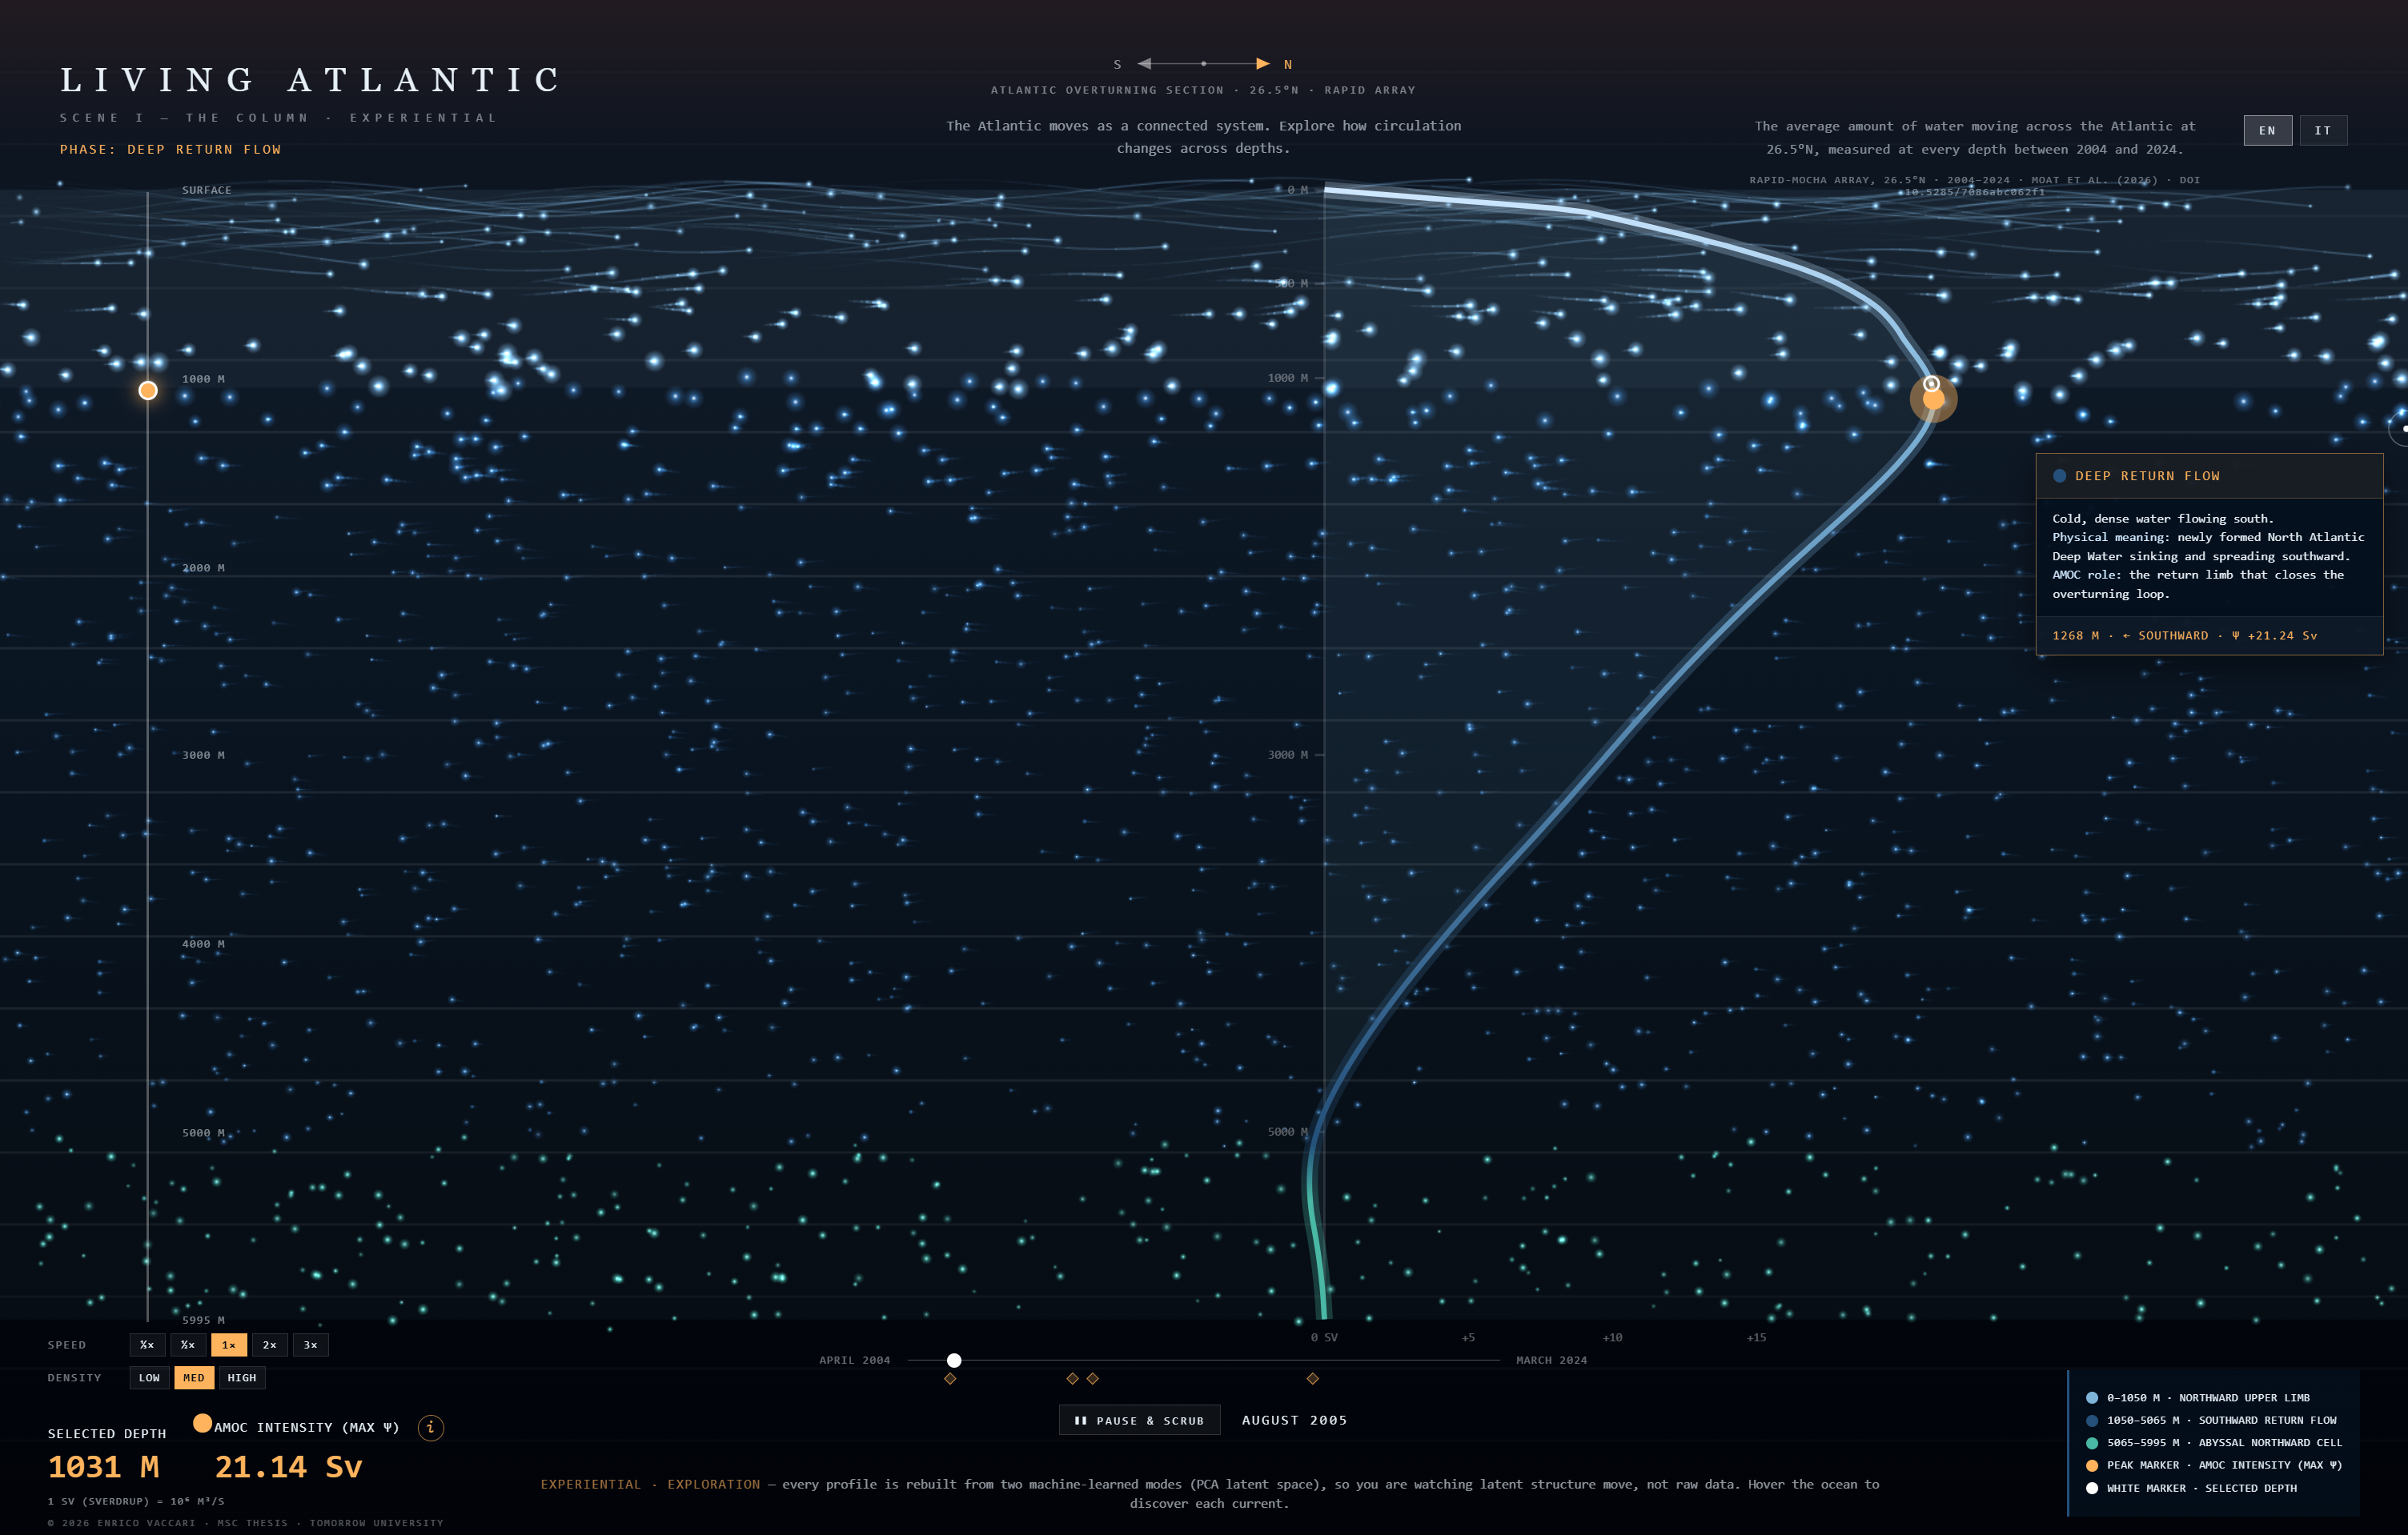
\includegraphics[width=\textwidth]{figures/viz1/viz1_column-experiential.png}
    \caption{Experiential (C2+C3): the same column set in motion.}
    \label{fig:thecolumn-experiential}
  \end{subfigure}

  \caption[The two conditions of Scene~I]{The two administered conditions of
  Scene~I, generated from the same data bundle through the same reconstruction
  function. The experiential condition introduces temporal behaviour while
  preserving the underlying structure of the static representation.}

  \label{fig:thecolumn-conditions}
\end{figure}

\paragraph{Obiettivo.} Stabilire che l'Atlantico a \ang{26.5}~nord non è una corrente con una posizione ma una quantità distribuita sulla profondità, le cui parti si muovono in direzioni opposte nello stesso momento. Un osservatore che esce sapendo solo che la circolazione è forte o debole non ha ricevuto l'affermazione.

\paragraph{Strategia di rappresentazione.} Il profilo canonico contiene il contro-flusso ma non lo mostra. Per vedere il moto opposto nella curva, un lettore deve sapere che la direzione del flusso a qualsiasi profondità è data dalla \emph{pendenza} della linea anziché dalla sua altezza --- dove la curva sale l'acqua va a nord, dove scende, a sud --- e deve leggere quella pendenza a occhio.

Gli specialisti lo fanno senza accorgersene; i non esperti, come la \S\ref{sec:empirical-viz} ha mostrato, in gran parte no \parencite{harold2016, mcmahon2015, fischer2020}. La Scena~I quindi non aiuta l'osservatore a calcolare la derivata; rende la derivata non necessaria, sostituendo l'inferenza con il movimento.

\paragraph{Mappatura.} L'informazione più importante qui è la struttura verticale (P0), perciò prende la posizione spaziale lungo i 307 livelli di profondità (P1).\footnote{I livelli coprono 0--5995,1\,m e sono quasi uniformemente spaziati, a un intervallo medio di 19,59\,m e un rapporto massimo-minimo di 1,03. La visualizzazione non corregge alcuna non uniformità che non sia nei dati.} Il contro-flusso diventa un campo di particelle avvettato dalla velocità meridionale locale (P2), i mesi anomali diventano disturbo di texture valutato dall'Isolation Forest del Capitolo~\ref{ch:data_pipeline} (P3), e $\mathrm{pc}_1$ guida un impulso sintetizzato, disattivato di default (P5). P4 è assente: la scena mostra una traiettoria e non ha incertezza da codificare. La Tabella~\ref{tab:ledger} registra ciascun elemento rispetto alla sua fonte nel bundle.

Il campo di particelle è guidato dalla derivata, mai da $\Psi$ stessa: guidarlo da $\Psi$ muoverebbe le particelle più velocemente proprio dove la velocità vera è zero, e non potrebbe affatto raffigurare un rovesciamento. I due confini non coincidono e non devono: $\Psi \to 0$ segna dove il trasporto cumulato svanisce (4346,1\,m), mentre $v \to 0$ segna dove il flusso locale si inverte (1050,4\,m e 5065,4\,m).\footnote{Nel profilo medio il picco di 16,808\,Sv sta a 1030,70\,m, con il primo livello diretto a sud immediatamente sotto. Gli ancoraggi di velocità sono riportati alla risoluzione della griglia: la derivazione restituisce il primo livello dove $v$ cambia segno anziché uno zero interpolato. L'attraversamento dello zero di $\Psi$ è riportato in entrambi i modi: 4346,1\,m alla risoluzione della griglia, 4340,85\,m interpolato.}

\paragraph{Condizioni.} C1 è l'idioma canonico: $\Psi$ in funzione della profondità, profondità verso il basso, griglia da pubblicazione, picco segnato, e nient'altro. C2+C3 è la stessa colonna messa in movimento.

C1 non è un confronto indebolito: è tratta dallo stesso bundle attraverso la stessa ricostruzione agli stessi 307 livelli, e il suo marcatore di picco riporta 16,808\,Sv a 1030,70\,m rispetto ai 16,9\,Sv a 1030\,m pubblicati per questo array \parencite{smeed2018}.

\paragraph{Fedeltà.} Ogni profilo in entrambe le condizioni è ricostruito attraverso l'Equazione~\ref{eq:reconstruction}, e l'identità che rende C1 empirica è quella registrata nella \S\ref{subsec:fidelity}.

\paragraph{Dove entra il modello.} Il contributo è duplice. La figura statica è una media di vent'anni, e le medie non si muovono; $\mathrm{pc}_1$ e $\mathrm{pc}_2$ rendono ogni mese un punto, così che camminare tra i punti ricostruisca ogni mese a sua volta. Il movimento non è quindi un'animazione aggiunta a una figura ma il modello che percorre la sua traiettoria appresa, con H2 che rende quel percorso fedele anziché comodo. Il modello segnala anche quali mesi si discostano dal record, che diventano texture; tutto il resto --- campo di particelle, assi, lettura del picco --- è classico.

\paragraph{Contributo atteso.} C1 mostra dove l'Atlantico è forte in media. C2 mostra ciò che C1 contiene ma non può mostrare. C3 aggiunge il tempo che il modello ha appreso: la colonna si gonfia verso 24,26\,Sv a gennaio~2018 e collassa verso 5,71\,Sv a marzo~2013, circa $3.5\sigma$ sotto la media dei massimi mensili, e il picco migra mentre procede --- 1070,2\,m nel mese più forte, 991,1\,m nel più debole.
\footnote{La migrazione è il secondo modo all'opera: $\mathrm{pc}_1$ fissa quanta acqua la colonna trasporta, $\mathrm{pc}_2$ la ridistribuisce verticalmente. Una bozza precedente di questa tesi affermava che la profondità del trasporto massimo è stabile mentre la sua entità varia; valutato lungo il record, non è così.} L'affermazione non è che la condizione esperienziale sia più attraente, ma che ciò che l'idioma statico non riesce a trasmettere --- struttura che va inferita, cambiamento che va immaginato --- è ciò che il movimento e il tempo latente consegnano direttamente.

\subsection{Scena II: La sala macchine}
\label{subsec:scene-engine}

\begin{quote}
\textbf{Domanda guida.} \emph{Guardando l'oceano muoversi da stato a stato nel tempo, va sempre da qualche parte di nuovo, oppure a volte ripassa per dove è già stato?}
\end{quote}

\begin{figure}[htbp]
  \centering

  \begin{subfigure}[t]{0.48\textwidth}
    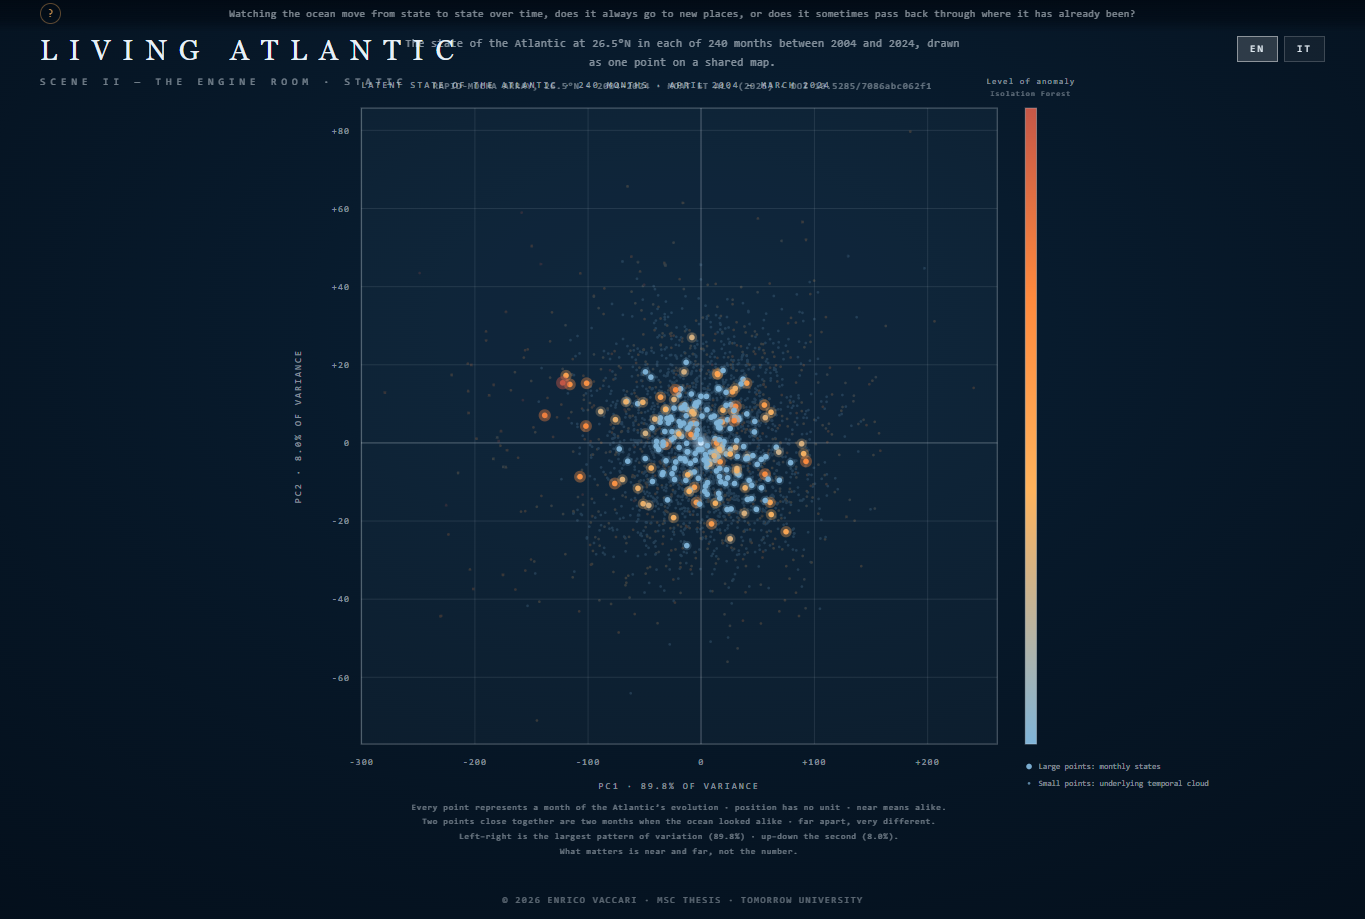
\includegraphics[width=\textwidth]{figures/viz2/viz2_theengine-static.png}
    \caption{Control (C1): the static latent-space representation.}
    \label{fig:theengine-static}
  \end{subfigure}
  \hfill
  \begin{subfigure}[t]{0.48\textwidth}
    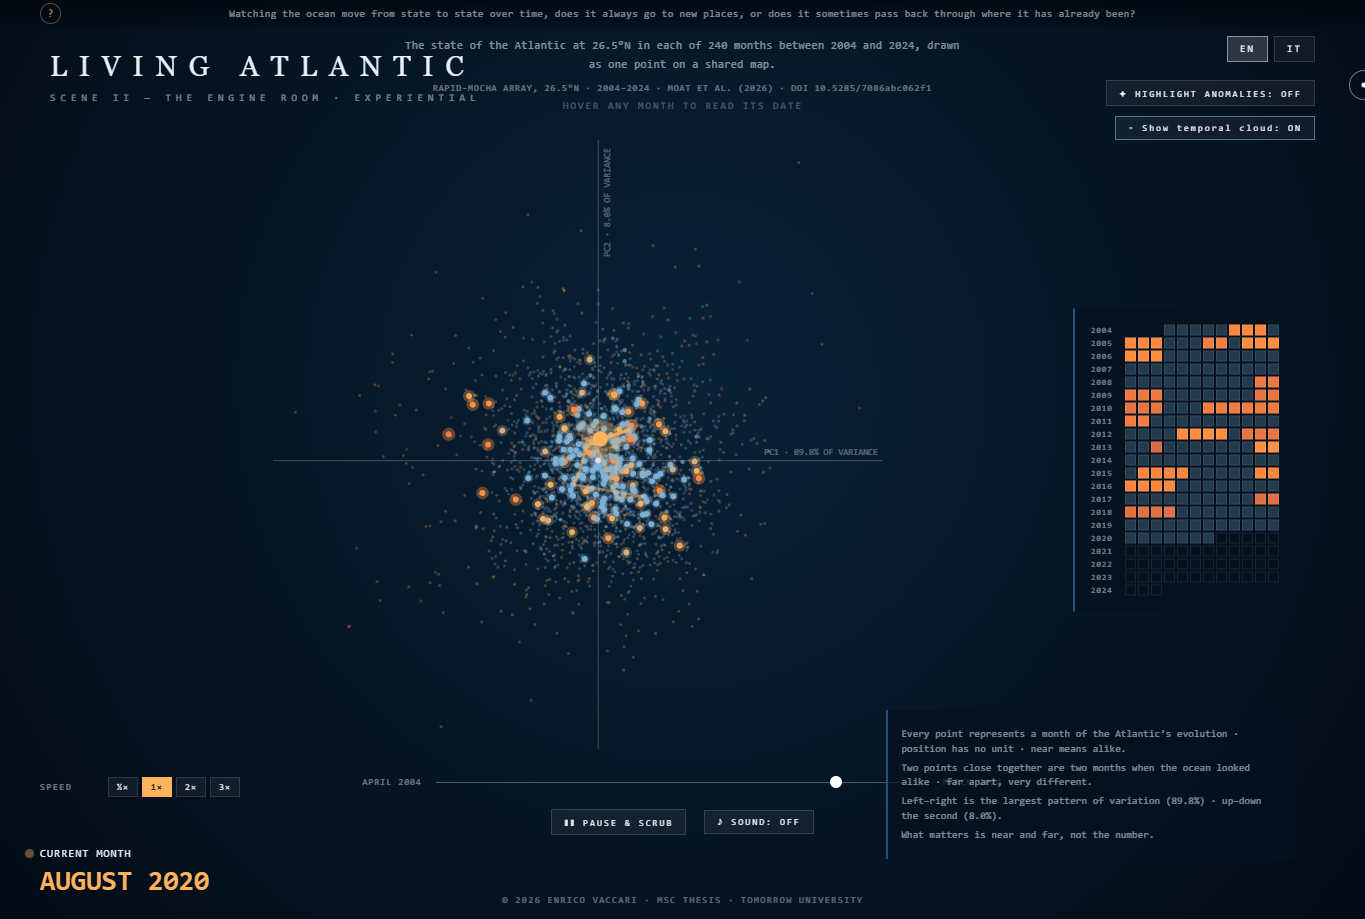
\includegraphics[width=\textwidth]{figures/viz2/viz2_theengine-experiential.png}
    \caption{Experiential (C2+C3): the evolving trajectory through latent space.}
    \label{fig:theengine-experiential}
  \end{subfigure}

  \caption[The two conditions of Scene~II]{The two administered conditions of
  Scene~II, drawn from the same latent coordinates in the data bundle. The
  static condition shows the monthly states as a fixed scatter; the
  experiential condition walks the same states in time.}

  \label{fig:theengine-conditions}
\end{figure}

\paragraph{Obiettivo.} Rendere il piano latente del Capitolo~\ref{ch:data_pipeline} uno spazio abitabile anziché uno strumento d'analista. Ogni mese del record è un punto, e la prossimità significa somiglianza. L'affermazione che la scena deve consegnare è che il sistema, lasciato vagare, ritorna: ripassa per stati che ha già occupato.\footnote{Questa ricorrenza caratterizza le dinamiche del presente record osservativo, in cui l'AMOC oscilla entro un regime stabile plasmato dal forzante stagionale e dalla variabilità interna. Non è evidenza che il sistema non possa subire transizioni di lungo periodo.}

\paragraph{Strategia di rappresentazione.} Il modo canonico di mostrare uno spazio latente è uno scatter di punti colorati per tempo \parencite{sacha2018}. Quella figura contiene la ricorrenza ma non può mostrarla: due punti possono stare quasi uno sull'altro pur distando anni, e una nuvola statica non dà all'occhio alcun modo di sapere che il percorso ha lasciato l'uno ed è poi arrivato all'altro. La ricorrenza è una proprietà della traiettoria, non dell'insieme di punti. La Scena~II percorre quindi il cammino nel tempo e accumula gli stati visitati come una nuvola.

\paragraph{Mappatura.} Ogni mese prende una posizione nel piano $\mathrm{pc}_1 \times \mathrm{pc}_2$, con gli assi etichettati con la varianza che ciascun modo spiega (P1). Il tempo diventa movimento reale lungo il percorso, e l'entità del cambiamento da mese a mese diventa la violenza visibile di ciascun passo (P2): i passi più grandi sono quattro volte la mediana, e quella variazione è segnale anziché rumore da lisciare.\footnote{I tre passi più grandi cadono su mesi che la fase di rilevamento segnala indipendentemente come anomali --- una coerenza interna registrata nell'Appendice~\ref{app:code}, non un'affermazione fatta a schermo.} I mesi anomali agitano il marcatore (P3) e $\mathrm{pc}_1$ guida il suono (P5); P4 è di nuovo assente.

\paragraph{Condizioni.} C1 è lo scatter canonico: i 240 mesi nel piano, colorati per livello di anomalia --- il punteggio Isolation Forest di ciascun mese, come registra la barra dei colori --- statico, non annotato e privo di ogni ordinamento nel tempo, così che un osservatore non abbia nulla con cui tracciare un ritorno. C2+C3 sono gli stessi punti, dati e colori, messi in movimento. Entrambe le condizioni mostrano la stessa nuvola sub-mensile più fine dietro i punti mensili, così che un mese si legga come la media di uno sciame inquieto anziché come un singolo stato.\footnote{Da \texttt{manifold\_cloud} nel bundle. La colorazione di anomalia è presa dal punteggio Isolation Forest del mese di ciascun punto, non dalla distanza dal centroide della nuvola; un surrogato spaziale codificherebbe ``lontano dal centro'' come ``raro'', che è parte della lettura che la scena deve trattenere.} Nessuna delle due condizioni disegna il profilo ricostruito: collegare il piano alla colonna darebbe al gruppo sperimentale informazione che il controllo non ha.

\paragraph{Fedeltà.} Il segno di ciascuna componente principale è arbitrario, perciò entrambe le condizioni rendono il piano con orientamento identico --- la nuvola che un partecipante di controllo vede è la stessa nuvola, non la sua immagine speculare --- e unità uguali su entrambi gli assi mantengono la distanza a schermo uguale alla distanza nello spazio latente.

\paragraph{Dove entra il modello.} Qui il modello non è substrato ma terreno. Il piano non esiste in natura: è la base che la decomposizione ha trovato, e ogni posizione in esso è una proiezione appresa. La Scena~I usava le coordinate latenti per animare un oggetto fisico; la Scena~II rende il sistema di coordinate stesso l'oggetto dell'attenzione, che è il passo dall'analisi esperta alla comunicazione pubblica che la \S\ref{sec:translate-premise} rivendica. La ricorrenza che un partecipante cerca è una proprietà di quello spazio appreso, percepibile solo perché H2 ha stabilito che lo spazio è abbastanza piatto da essere percorso senza distorsione. A differenza della Scena~I, nulla qui esisterebbe senza il modello.

\paragraph{Contributo atteso.} Lo scatter statico mostra che l'Atlantico occupa un insieme limitato di stati; la condizione esperienziale mostra ciò che esso contiene ma non può mostrare --- che il sistema si muove attraverso quell'insieme con struttura, alla deriva in certi momenti e a scatti in altri, e che ritorna.

\subsection{Scena III: La soglia}
\label{subsec:scene-threshold}

\begin{quote}
\textbf{Domanda guida.} \emph{Pensi che quanto i modelli concordano tra loro sia rimasto lo stesso in tutti gli anni, o sia cambiato?}
\end{quote}

\begin{figure}[htbp]
  \centering

  \begin{subfigure}[t]{0.48\textwidth}
    \vspace{0pt}
    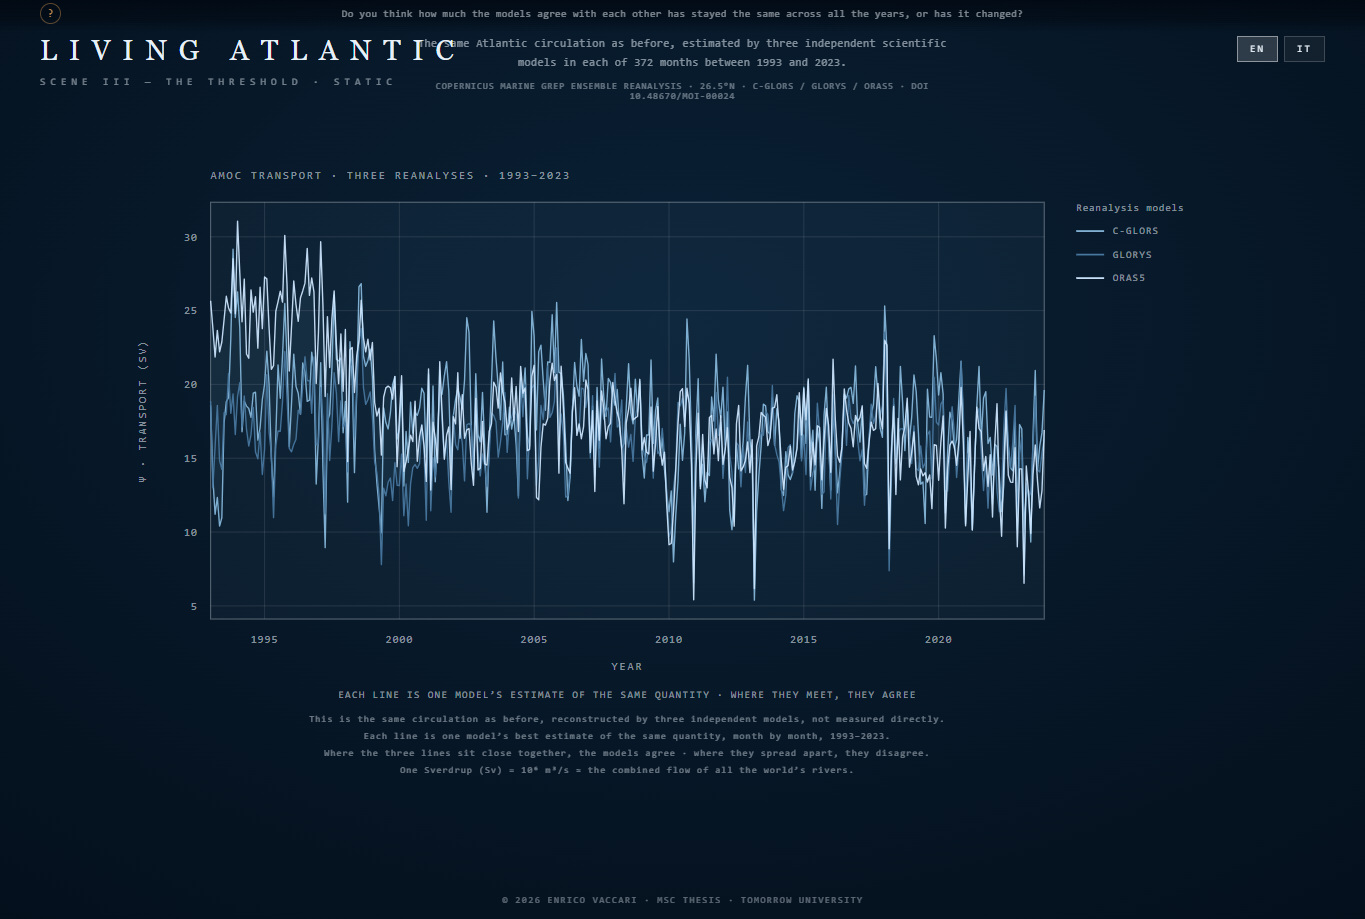
\includegraphics[width=\textwidth]{figures/viz3/viz3_thethreshold-static.png}
    \caption{Control (C1): the three reanalysis series, static.}
    \label{fig:thethreshold-static}
  \end{subfigure}
  \hfill
  \begin{subfigure}[t]{0.48\textwidth}
    \vspace{0pt}
    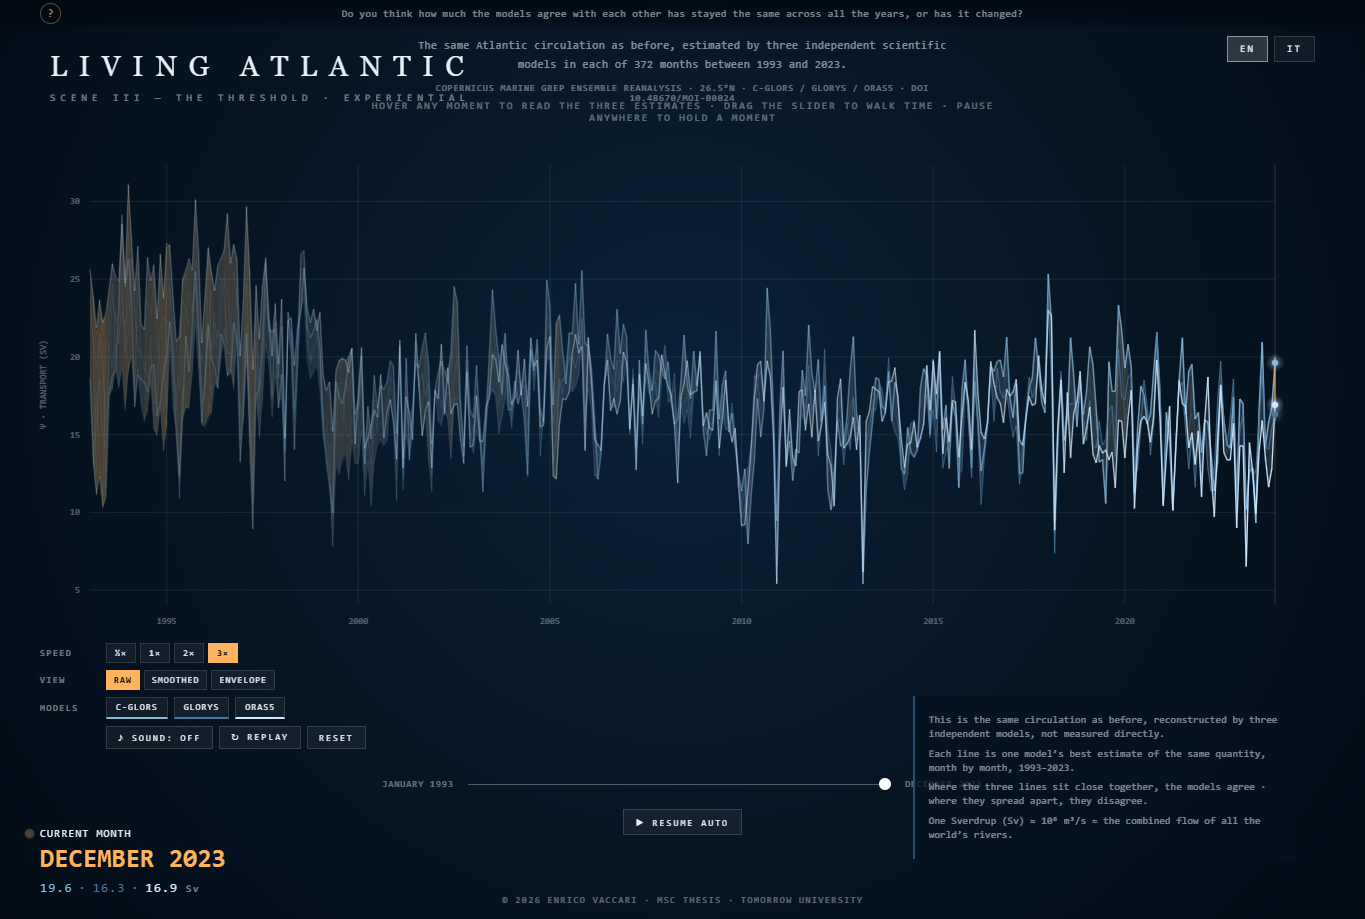
\includegraphics[width=\textwidth]{figures/viz3/viz3_thethreshold-experiential.png}
    \caption{Experiential (C2+C3): the same series, with their disagreement rendered as motion.}
    \label{fig:thethreshold-experiential}
  \end{subfigure}

  \caption[The two conditions of Scene~III]{The two administered conditions of
  Scene~III, drawn from the same three Copernicus reanalysis members. The
  static condition shows the three series at once; the experiential condition
  renders their changing disagreement as motion and sound.}

  \label{fig:thethreshold-conditions}
\end{figure}

\paragraph{Obiettivo.} Rendere l'incertezza una qualità sentita anziché un numero. Le Scene~I e~II mostravano una quantità misurata da un array nell'acqua; la Scena~III mostra la stessa quantità ricostruita in tre modi diversi, da tre rianalisi oceaniche che concordano nel presente e divergono nel passato.\footnote{Rianalisi d'ensemble Copernicus Marine GREP, membri C-GLORS, GLORYS e ORAS5, mensile da gennaio~1993 a dicembre~2023.}

\paragraph{Strategia di rappresentazione.} L'idioma canonico traccia l'ensemble come una media con una banda ombreggiata, o come linee dei membri sovrapposte. Entrambi contengono il mutevole disaccordo ma lo presentano come una distanza da misurare tra le curve --- il compito inferenziale che la Scena~I si propone di rimuovere. La Scena~III rende invece il disaccordo una proprietà del medium: dove le ricostruzioni convergono il display è calmo, dove divergono diventa visibilmente e udibilmente agitato. Questo realizza P4, tenuto in riserva per le prime due scene, e con esso DP2.2: il mutevole disaccordo è reso come variazione percettiva anziché come annotazione numerica.

\paragraph{Mappatura.} La quantità più importante qui non è il valore di trasporto ma il mutevole disaccordo, perciò prende il canale più forte e diventa movimento (P0). La stima di ciascun membro tiene una posizione nel tempo (P1), che a sua volta diventa movimento reale (P2). L'incertezza diventa variabilità animata (P4): turbolenza, larghezza della banda e temperatura di colore scalano tutte con la dispersione reale tra i membri a ciascun mese, e nessuna è mai stampata come numero. La stessa dispersione guida una texture audio, pulita quando i modelli concordano e che si fa ruvida mentre si separano (P5). P3 è assente, non essendo l'anomalia centrale all'affermazione.

\paragraph{Condizioni.} C1 disegna le tre linee dei membri nel tempo, distinguibili e nominate, statiche e non annotate: nessuna epoca è ombreggiata, nessun anno segnato. C2+C3 mette le stesse linee in movimento e aggiunge il medium vivente tra esse, con controlli che permettono a un osservatore di rivedere dati identici a diverse aggregazioni --- grezzi, lisciati su una finestra scelta, o il solo inviluppo --- e isolare una qualsiasi singola rianalisi.\footnote{Queste sono viste di un unico dataset, non informazione aggiuntiva: ogni aggregazione è calcolata dalle stesse tre serie dei membri, e i valori grezzi restano disponibili in entrambe le condizioni.}

\paragraph{Fedeltà.} Ogni proprietà visiva e uditiva è guidata dalla dispersione reale tra i tre membri a ciascun mese, e nessuna aggregazione introduce una quantità che i membri non contengono. Le tre linee non sono mai ridotte a una media con barre d'errore: il soggetto della scena sono tre ricostruzioni in disaccordo, non una stima con un margine.

\paragraph{Dove entra il modello.} Meno delle tre, e l'asimmetria è istruttiva. Le tre rianalisi sono modelli oceanici fisici prodotti da altre istituzioni, non rappresentazioni apprese costruite per questa tesi, e la dispersione tra esse è aritmetica: il contributo di machine learning del Capitolo~\ref{ch:data_pipeline} non guida questa scena. Ciò che si trasferisce è la grammatica anziché il modello --- gli stessi principi che mappavano la struttura latente sul movimento nelle Scene~I e~II qui mappano il disaccordo d'ensemble su variabilità animata, senza uno spazio latente su cui poggiare. Che la grammatica sopravviva alla rimozione del modello è l'evidenza più forte disponibile entro questa tesi per l'obiettivo~O2.2.

\paragraph{Contributo atteso.} Il grafico statico mostra che tre modelli stimano la stessa quantità e non concordano del tutto; la condizione esperienziale mostra che il grado di accordo è esso stesso una variabile --- le ricostruzioni che si separano nel record più antico e convergono man mano che il vincolo osservativo migliora, con la dispersione media che si dimezza all'incirca tra il decennio pre-2004 e gli anni dell'array.\footnote{Il restringimento è graduale anziché un gradino all'installazione dell'array, e l'artefatto non segna alcuna data; il cambiamento è lasciato da percepire anziché annunciato.} Se un non specialista legga quel cambiamento come un cambiamento di certezza --- anziché come una variazione decorativa --- è ciò che l'aspettativa~E3.2 verifica.

% ============================================================
% Tabella riassuntiva
% ============================================================
\begin{table}[tbp]
\centering
\caption[Le tre scene a colpo d'occhio]{Le tre scene di \emph{Living Atlantic}: la domanda che ciascuna pone all'osservatore, i principi che realizza, e ciò che il machine learning contribuisce. Il contributo diminuisce lungo la discesa --- e la sopravvivenza della grammatica fino alla Scena~III, dove nessun modello appreso guida il display, è l'evidenza della sua trasferibilità (O2.2).}
\label{tab:scene-summary}
\small
\renewcommand{\arraystretch}{1.35}

\begin{tabularx}{\textwidth}{@{}p{2.6cm} X p{2.5cm} X@{}}
\toprule
\textbf{Scena} &
\textbf{Domanda guida} &
\textbf{Principi} &
\textbf{Cosa aggiunge il ML} \\
\midrule

\makecell[l]{Scena I\\La colonna} &
L'acqua si muove tutta allo stesso modo; se no, in quali direzioni? &
P0, P1, P2, P3, P5 &
Le coordinate latenti lungo cui il profilo si muove, e i punteggi di anomalia che ne disturbano la texture. Il campo di particelle è classico. \\

\makecell[l]{Scena II\\La sala macchine} &
L'oceano va sempre verso qualcosa di nuovo, o ripassa per dove è già stato? &
P1, P2, P3, P5 &
Il piano stesso: lo spazio percorso è la base appresa. Nulla nella scena esiste senza il modello. \\

\makecell[l]{Scena III\\La soglia} &
L'accordo tra i modelli è rimasto lo stesso negli anni, o è cambiato? &
P0, P1, P2, P4, P5 &
Il minore dei tre. Le rianalisi sono modelli fisici esterni; la grammatica porta la scena senza uno spazio appreso. \\

\bottomrule
\end{tabularx}
\end{table}


\setpartsubtitle{Capire l'impatto della rappresentazione}
\part{VALUTARE}
% =========================================================================
% CAPITOLO 8 — VALUTARE: LO STUDIO CON UTENTI
% =========================================================================

\chapter{Studio con utenti}
\label{ch:userstudy}

\noindent
{\rmfamily\itshape
\begin{tabular}[t]{@{}l@{\hspace{0.3cm}}p{12.5cm}@{}}
\textls[50]{\textbf{Trattati:}} &
\textls[50]{Test e validazione · Disegno tra soggetti · Strumento del questionario · Protocollo
di comprensione scritta · Quadro di codifica · Consenso ed etica · Limiti del disegno}
\end{tabular}
}

\vspace{0.5cm}

Il Capitolo~\ref{ch:translate} ha sviluppato l'artefatto e ha mostrato che le due condizioni sono allineate per provenienza, inquadramento e unità di misura, differendo deliberatamente in un aspetto: la condizione esperienziale porta la dimensione temporale che quella statica trattiene, che è la variabile che lo studio si propone di esaminare. La domanda successiva è se presentarla in modi diversi incida su come le persone la comprendono. Lo studio non mira a dimostrare che la visualizzazione esperienziale sia migliore; esamina se un piccolo gruppo di partecipanti per lo più non specialisti comprenda il sistema in modo diverso sotto una visualizzazione statica o una esperienziale, ed è progettato così che tanto risultati positivi quanto negativi informino lo stadio successivo. È uno \emph{studio socio-cognitivo}, rivolto a come le persone interpretano le visualizzazioni anziché a testare la scienza sottostante o la competenza dei partecipanti.

% -------------------------------------------------------------------------
\section{Scopo}
\label{sec:eval-purpose}

I Capitoli~\ref{ch:data_pipeline} e~\ref{ch:translate} hanno affrontato rilevamento e traduzione. Il passo restante era mettere le due forme di rappresentazione davanti ai partecipanti e confrontare come vengono comprese --- ciò che la domanda di ricerca centrale (\S\ref{sec:rqs}) chiede --- perciò era richiesto uno \emph{studio comparativo con utenti}. Poiché le visualizzazioni animate possono apparire più efficaci semplicemente perché portano informazione che la versione statica non ha \citep{tversky2002}, lo studio allinea le due condizioni per provenienza, inquadramento e unità di misura e varia solo la forma.

% -------------------------------------------------------------------------
\section{Un primo stadio esplorativo}
\label{sec:eval-exploratory}

Lo studio è esplorativo per disegno. Hanno partecipato venticinque persone, dodici assegnate alla condizione statica e tredici all'esperienziale.\footnote{La differenza tra dodici e tredici deriva dall'assegnazione casuale a una piccola dimensione campionaria. Non incide su nulla nell'analisi descrittiva oltre i denominatori usati nel Capitolo~\ref{ch:results}.}

La dimensione campionaria è stata fissata a priori, su basi di fattibilità e dell'obiettivo esplorativo. Un criterio di saturazione non è rivendicato e non si adatterebbe: la saturazione appartiene ai disegni induttivi e generativi di teoria, mentre questa analisi è deduttiva rispetto a una griglia fissata prima di leggere le risposte \citep{braunclarke2021}.

Il criterio difendibile è l'\emph{information power} \citep{malterud2016}: uno studio qualitativo ha bisogno di meno partecipanti man mano che il suo obiettivo si restringe, il suo campione si fa più specifico, il suo fondamento si rafforza e la sua analisi lavora per categorie. Questo studio è ristretto nell'obiettivo, specifico nel campione, fondato sulla griglia di codifica del Capitolo~\ref{ch:literature} e analizzato per categoria --- una configurazione per cui venticinque partecipanti portano adeguata information power, e nessuna per l'inferenza su scala di popolazione che lo studio non tenta.

Questo primo studio individua invece pattern iniziali per la ricerca futura: quali concetti i partecipanti comprendono, quali sono comunemente fraintesi, se le due condizioni sembrino portare a interpretazioni diverse, e se l'approccio sia abbastanza promettente da giustificare uno studio più ampio e statisticamente potente.

% -------------------------------------------------------------------------
\section{Partecipanti e pubblico}
\label{sec:eval-audience}

Lo studio si rivolgeva a non specialisti: partecipanti senza formazione specifica in oceanografia, scienza del clima, matematica o machine learning. Lo status di non specialista è stato stabilito per auto-dichiarazione nella sezione di background. Ciò riflette l'obiettivo della tesi: le visualizzazioni sono intese a sostenere la comprensione di sistemi complessi oltre il pubblico specializzato.

Non ci si aspettava che i partecipanti avessero conoscenza pregressa dell'AMOC o dei concetti usati nelle visualizzazioni; il questionario forniva l'informazione di base necessaria ad affrontare le scene. Il reclutamento è avvenuto attraverso reti personali in italiano e in inglese, perciò il campione è di convenienza: la sua composizione è descritta nella \S\ref{sec:res-sample} e le sue implicazioni nella \S\ref{sec:eval-limitations}.

% -------------------------------------------------------------------------
\section{Lo strumento}
\label{sec:eval-instrument}

Lo studio è stato condotto come questionario scritto autoguidato tramite Google Forms. Sono state usate quattro versioni del questionario, combinando due lingue (italiano e inglese) con le due condizioni sperimentali (statica ed esperienziale).\footnote{Le quattro versioni usano la stessa formulazione entro ciascuna lingua e differiscono solo nei link alle scene che conducono alle visualizzazioni statiche o esperienziali. I protocolli completi del questionario sono forniti nell'Appendice~\ref{app:protocols}.}

% it/figures/user_study/Google_Form.tex — versione italiana
\begin{figure}[htbp]
    \centering
    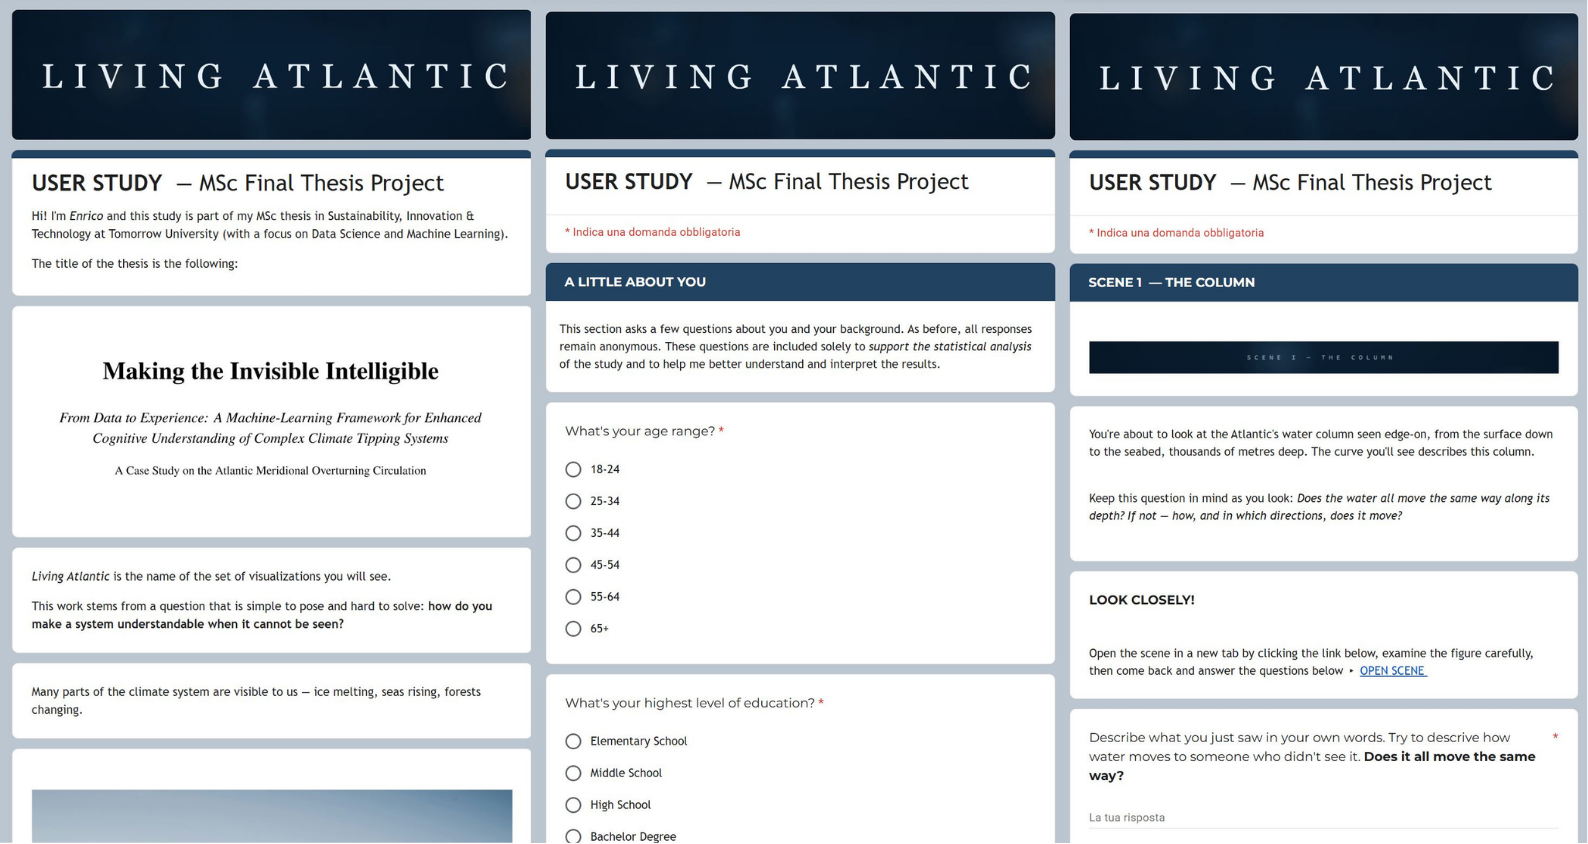
\includegraphics[width=\textwidth]{figures/user_study/Google_Form.png}
    \caption[Il questionario dello studio in Google Forms]{Il Google Form usato per la
    raccolta dati, che mostra l'introduzione, gli item di background e il blocco della
    prima scena. Il modulo raccoglieva descrizioni scritte di ciascuna scena e
    valutazioni di fiducia.}
    \label{fig:google-form}
\end{figure}


Un questionario scritto e auto-somministrato è stato preferito a un protocollo think-aloud con sessioni dal vivo: raggiunge più partecipanti e dà a tutti le stesse istruzioni senza che un intervistatore influenzi le risposte.

Il questionario segue un'unica sequenza: introduzione, consenso, informazioni sull'anonimato, una breve sezione di background e il contesto di base necessario a comprendere l'AMOC e lo sverdrup --- tutto identico per entrambi i gruppi. Le tre scene seguono poi in ordine (\textit{La colonna}, \textit{La sala macchine}, \textit{La soglia}). Per ciascuna, i partecipanti ricevono una breve introduzione e una domanda guida, aprono la visualizzazione assegnata, la esplorano e, al ritorno, rispondono a domande aperte con parole proprie. Una riflessione finale e un debriefing chiudono il questionario.

L'ordine delle domande è intenzionale: i partecipanti descrivono ciò che hanno compreso con parole proprie prima che sia chiesto loro di valutare la propria fiducia o di riflettere sull'esperienza, e la struttura a due condizioni è spiegata solo dopo che le risposte principali sono state raccolte.

% -------------------------------------------------------------------------
\section{Le condizioni dello studio}
\label{sec:eval-conditions}

I due gruppi differivano solo nel tipo di visualizzazione esperita. Entrambi hanno visto le stesse tre scene --- \textit{La colonna}, \textit{La sala macchine} e \textit{La soglia} --- con le stesse domande e le stesse informazioni contestuali; il gruppo di controllo ha visto ciascuna come visualizzazione statica convenzionale, il gruppo esperienziale come la sua controparte interattiva e dinamica.\footnote{Il disegno delle tre scene, e la distinzione tra le loro componenti derivate dal machine learning e quelle classiche, è descritto nella \S\ref{sec:three-scenes}. Il Capitolo~\ref{ch:translate} stabilisce che entrambe le condizioni usano lo stesso bundle di dati, la stessa funzione di ricostruzione e la stessa provenienza.}

Una precisazione conta: il machine learning non genera ogni elemento delle condizioni esperienziali --- il campo di particelle della Scena~I è una derivata, la dispersione della Scena~III viene da modelli oceanici esterni --- perciò lo studio confronta due modi di presentare lo stesso sistema, non una condizione di machine learning contro una non di machine learning.

% -------------------------------------------------------------------------
\section{Randomizzazione e debriefing}
\label{sec:eval-randomisation}

I partecipanti sono stati assegnati casualmente a una delle due condizioni. Con un piccolo campione, la randomizzazione non può garantire gruppi bilanciati, ma rimuove l'autoselezione in una condizione e così limita una fonte sistematica di bias. Ogni partecipante è rimasto nella condizione assegnata fino alla fine dello studio principale, così che l'esposizione all'alternativa non potesse influenzare le sue risposte.\footnote{Mantenere la struttura sperimentale non svelata fino alla fine riduce anche la possibilità che i partecipanti interpretino la propria esperienza come parte di un confronto e aggiustino di conseguenza le risposte.}

Una volta raccolte tutte le risposte principali, il debriefing ha spiegato la struttura, introdotto le due condizioni e dato a ogni partecipante accesso all'insieme completo delle visualizzazioni --- inclusa la versione che non aveva esperito.

% -------------------------------------------------------------------------
\section{Sezione di background}
\label{sec:eval-demographics}

Una breve sezione di background prima dei compiti ha raccolto fascia d'età, istruzione, ambito di studio o lavoro e familiarità auto-valutata con la scienza del clima, l'AMOC e le visualizzazioni di dati.

Il suo scopo è descrittivo: dato il piccolo campione, queste variabili descrivono il pubblico e inquadrano i risultati anziché alimentare una modellazione statistica.

% -------------------------------------------------------------------------
\section{Consenso, anonimato ed etica}
\label{sec:eval-ethics}

La partecipazione era volontaria e anonima: il questionario non ha raccolto nomi, indirizzi email o altri identificatori diretti, i partecipanti potevano interrompere in qualsiasi momento senza dare una ragione, e il consenso è stato ottenuto prima dell'inizio dello studio attraverso una conferma esplicita che proseguire significava accettare di partecipare. Le risposte sono state usate solo per questa ricerca, e nessuna informazione identificativa compare nel Capitolo~\ref{ch:results}. Il testo di consenso e anonimato è riprodotto nell'Appendice~\ref{app:protocols}; gli impegni etici che attua sono esposti nella \S\ref{sec:ethics-statement} e nell'Appendice~\ref{app:ethics-conduct}.

% -------------------------------------------------------------------------
\section{Quadro di valutazione}
\label{sec:eval-framework}

Le risposte aperte sono analizzate rispetto a una griglia di codifica predefinita. Lo scopo non è segnare le risposte come giuste o sbagliate ma identificare se i partecipanti esprimano l'idea strutturale principale che ciascuna scena rappresenta.\footnote{La griglia completa, incluso il target di ciascuna scena e la definizione di ciascuna categoria, è fornita nell'Appendice~\ref{app:protocols}.}

Le categorie sono state definite prima di analizzare le risposte, e ciascuna è legata alla domanda guida della sua scena (\S\ref{sec:three-scenes}): direzioni opposte a profondità diverse per la Scena~I, ricorrenza tra stati per la Scena~II, e cambiamento nel livello di accordo tra i tre modelli per la Scena~III. Una risposta conta come dimostrazione di comprensione solo quando il partecipante descrive la struttura rilevante con parole proprie; menzionare movimento, colore o altre caratteristiche visive non è sufficiente.

La codifica è stata svolta attraverso una procedura assistita. Un large language model, istruito sulla griglia di codifica e sulle definizioni delle categorie, ha prodotto un'etichetta iniziale per ciascuna risposta. Il ricercatore ha poi riesaminato ogni etichetta e l'ha corretta ovunque il proprio giudizio differisse dalla proposta automatica. La codifica finale è quindi il risultato di un'adjudicazione umana, con il passaggio automatico che funge solo da punto di partenza. In questo studio la revisione ha mantenuto ognuna delle 75 etichette del modello, perciò il tasso di override è stato nullo. Un accordo completo di questo tipo è coerente con una griglia chiara e ben specificata, ma di per sé non può essere separato dal rischio di ancoraggio che una procedura assistita comporta --- un revisore che vede prima l'etichetta proposta può confermarla anziché giudicarla da capo.\footnote{La griglia di codifica predefinita (Appendice~\ref{app:protocols}) è ciò che mantiene trasparente questa procedura: ogni etichetta può essere riverificata da altri usando i criteri fissi e le risposte originali. Non è riportato alcun coefficiente di accordo tra codificatori, poiché tale misura non si applica a un disegno a codificatore singolo supportato da un primo passaggio automatico. Il limite dell'analisi a codificatore singolo è discusso nella \S\ref{sec:eval-limitations}.}

Il quadro mantiene anche la comprensione dimostrata --- la descrizione scritta --- separata dalla comprensione percepita, la valutazione di fiducia, perché i partecipanti possono sentirsi sicuri anche quando la loro interpretazione non corrisponde alla struttura intesa.\footnote{\textcite{fischer2020} documenta casi in cui un'alta fiducia accompagna un'interpretazione errata. L'analisi quindi incrocia la fiducia con le risposte codificate anziché trattarla come prova di comprensione corretta.}

% -------------------------------------------------------------------------
\section{Cosa lo studio si aspetta di trovare}
\label{sec:eval-expectations}

Lo studio chiede se la condizione esperienziale sostenga una comprensione più chiara di quella statica, nei termini delle aspettative E3.1 ed E3.2 (\S\ref{sec:hypotheses}): se profondità e direzioni opposte diventino più facili da comprendere (Scena~I), la ricorrenza più facile da riconoscere (Scena~II), e i cambiamenti nell'accordo tra modelli più facili da percepire (Scena~III). Queste sono aspettative, non previsioni, e nessuna presume una direzione o un'entità dell'effetto.

% -------------------------------------------------------------------------
\section{Tempi e carico}
\label{sec:eval-burden}

Il questionario è stato progettato per richiedere da quindici a venti minuti: abbastanza breve da evitare affaticamento inutile, abbastanza lungo da esplorare tre visualizzazioni.

% -------------------------------------------------------------------------
\section{Limiti del disegno}
\label{sec:eval-limitations}

Lo studio ha diversi limiti importanti. Primo, il campione è piccolo (venticinque partecipanti) e leggermente sbilanciato (dodici statica, tredici esperienziale), e non fornisce potenza statistica sufficiente per un'analisi inferenziale forte o una generalizzazione su scala di popolazione.

Secondo, i partecipanti sono stati reclutati attraverso reti personali, rendendo il campione di convenienza. La sua età, il suo background e la sua esperienza possono quindi differire da quelli della più ampia popolazione che le visualizzazioni intendono in ultima analisi raggiungere.

Terzo, tutti i partecipanti hanno incontrato le tre scene nello stesso ordine fisso (I, II, III), scelto per le ragioni interpretative esposte nella \S\ref{sec:three-scenes}. Poiché quell'ordine non è stato controbilanciato, la posizione nella sequenza è confusa con l'identità della scena: qualsiasi confronto \emph{tra} scene porta un possibile contributo dall'apprendimento lungo la sequenza o dall'affaticamento verso la fine. Questo riguarda direttamente il risultato della Scena~III, dove la condizione esperienziale ha reso meno bene e dove il compito cadeva anche per ultimo in un questionario di quindici-venti minuti. Un secondo caveat specifico della Scena~III è che il briefing di controllo diceva ai partecipanti che la figura statica permetteva loro di ``vedere dove concordano e dove differiscono'', e l'item di comprensione (Q16) chiedeva direttamente se i tre modelli concordano o divergono nel tempo; entrambi possono aver suggerito la lettura di convergenza, offrendo un'ulteriore possibile ragione per cui la condizione di controllo ha raggiunto ogni partecipante. Controbilanciare l'ordine delle scene, e neutralizzare questi suggerimenti, è un requisito per qualsiasi replica più ampia.

Quarto, lo studio usa risposte scritte e auto-riportate. Ciò significa che l'analisi è limitata a ciò che i partecipanti sono in grado o disposti a esprimere per iscritto. Alcuni aspetti della comprensione possono quindi restare non osservati.

Quinto, le risposte sono state codificate da un singolo ricercatore con un primo passaggio automatico e senza un secondo codificatore indipendente, perciò non può essere riportata alcuna affidabilità tra codificatori e si applica il rischio di ancoraggio segnalato nella \S\ref{sec:eval-framework}. La griglia definita a priori mantiene ogni assegnazione aperta a una riverifica esterna rispetto a criteri fissi, ma non sostituisce una doppia codifica indipendente.

Sesto, le due condizioni pongono richieste diverse all'hardware del partecipante. La condizione esperienziale anima di continuo e riproduce audio in tempo reale, mentre quella statica no, perciò un dispositivo più lento degrada una condizione e non l'altra. Non sono state raccolte informazioni su dispositivo o browser, e questa asimmetria è quindi riconosciuta anziché controllata.

Settimo, il briefing condiviso della Scena~II descriveva il centro della nuvola di punti come lo stato a cui l'oceano ``tende naturalmente a tornare''. Questo anticipa la ricorrenza che la scena chiede ai partecipanti di notare ed è fisicamente impreciso --- il centro è la media del record, non un equilibrio dinamico verso cui il sistema è richiamato --- perciò in qualsiasi replica serve una formulazione neutra.

Infine, lo studio distingue tra comprensione dimostrata e percepita. Un partecipante può riportare alta fiducia senza mostrare la comprensione strutturale attesa nella sua risposta scritta. Ciò non è trattato come un errore metodologico, ma come una distinzione importante che il quadro di valutazione è progettato per catturare.

% (Google_Form.tex era qui, orfano dopo l'ultima sezione; ora sta in 8.4)
Questi limiti non tolgono valore allo studio: fornisce un primo test empirico dell'approccio e individua pattern per guidare una replica più ampia, più controllata e statisticamente potente --- una base empirica iniziale anziché una validazione finale.

% =========================================================================
% CAPITOLO 9 — RISULTATI
% =========================================================================

\chapter{Risultati}
\label{ch:results}

\noindent
{\rmfamily\itshape
\begin{tabular}[t]{@{}l@{\hspace{0.3cm}}p{12.5cm}@{}}
\textls[50]{\textbf{Trattati:}} &
\textls[50]{Composizione del campione · Analisi descrittiva · Esiti della codifica · Comprensione
strutturale · Frequenza degli errori · Fiducia vs correttezza · Codici emergenti}
\end{tabular}
}

\vspace{0.5cm}

Questo capitolo riporta ciò che mostrano le risposte codificate: il campione, l'esito della codifica per ciascuna scena, la frequenza dell'errore sulla funzione di corrente, la relazione tra fiducia e correttezza, e la distribuzione dei codici emergenti tra le condizioni. La loro interpretazione, e la loro relazione con le aspettative del Capitolo~\ref{ch:userstudy}, è lasciata al Capitolo~\ref{ch:discussion}. Dato il campione di venticinque, tutte le cifre sono descrittive; i tre test esplorativi più sotto sono etichettati come tali e non sono trattati come inferenziali. Dimensioni dell'effetto e intervalli di confidenza non sono riportati: con dodici e tredici partecipanti per condizione i loro intervalli coprirebbero quasi tutto lo spazio dei parametri, e presentarli darebbe un'apparenza inferenziale a un confronto che questo capitolo non fa. L'artefatto la cui ricezione è qui riportata è documentato nel Capitolo~\ref{ch:translate}.\footnote{Tutti i conteggi e le tabelle di questo capitolo sono stati ricalcolati direttamente dall'insieme delle risposte codificate, conservato nel repository analitico documentato nella \S\ref{app:c-repos}.}

% -------------------------------------------------------------------------
\section{Composizione del campione}
\label{sec:res-sample}

Venticinque partecipanti hanno completato lo studio, dodici nella condizione di controllo e tredici nella sperimentale. La maggior parte aveva tra i 25 e i 34 anni (17 su 25). Il campione era molto istruito: quindici avevano una laurea magistrale, nove una triennale e uno un titolo di scuola secondaria superiore (Figura~\ref{fig:demographics}). Gli ambiti di studio e lavoro erano vari --- ingegneria, scienze, discipline umanistiche, sanità e arti --- senza alcun ambito rappresentato da più di due partecipanti.

La familiarità auto-valutata era bassa per il sistema specifico e moderata per le competenze correlate. La familiarità con l'AMOC era molto bassa (media 1,84 su una scala a dieci punti), quella con i temi climatici moderata (4,88), e quella con la lettura di visualizzazioni di dati la più alta delle tre (6,20).

Un controllo di equilibrio ha confrontato le due condizioni su queste misure (Figura~\ref{fig:balance}). Il gruppo sperimentale non era superiore a quello di controllo in nessuna di esse, ed era leggermente inferiore in tutte e tre; lo scarto maggiore era nella familiarità con le visualizzazioni di dati (5,54 contro 6,92 su una scala a dieci punti, una differenza di 1,38 punti).\footnote{Un confronto di Mann--Whitney colloca quello scarto a $p \approx 0.09$, riportato qui solo per completezza. L'entità e la direzione di uno squilibrio di partenza, non la sua significatività statistica, sono ciò che conta per l'interpretazione: un test di significatività sull'equilibrio di partenza risponde a una domanda che la randomizzazione ha già risolto.} La direzione conta: va nel verso che renderebbe più probabile l'errore della Scena~I nella condizione sperimentale (\S\ref{sec:res-misconception}), ed è ripresa nel Capitolo~\ref{ch:discussion}.


% -------------------------------------------------------------------------
\section{Comprensione strutturale per scena}
\label{sec:res-structure}

La quota di risposte codificate \emph{grasped} (colte) è variata nettamente tra le tre scene, e la direzione della differenza tra le condizioni non era la stessa in ciascuna (Figura~\ref{fig:grasped}).

Nella \textbf{Scena~I} (direzioni opposte con la profondità), le due condizioni erano vicine. Due terzi delle risposte di controllo (66,7\%) e una quota simile delle sperimentali (69,2\%) sono state codificate come grasped. Nella \textbf{Scena~II} (ricorrenza), nessun partecipante di controllo è stato codificato grasped (0 su 12), contro il 23,1\% nella condizione sperimentale (3 su 13); anche i codici \emph{partial} (parziale) sono aumentati nello stesso confronto, da due a cinque. Nella \textbf{Scena~III} (cambiamento nell'accordo tra modelli nel tempo), il pattern era invertito. Ogni partecipante di controllo è stato codificato grasped (12 su 12, 100\%), contro il 76,9\% nella condizione sperimentale (10 su 13).

Le risposte scritte mostrano ciò che i codici strutturali catturano. Nella Scena~I, una risposta grasped nominava direttamente l'inversione stratificata --- ``L'acqua non si muove in modo uniforme; vicino alla superficie e nella fascia medio-alta sembra più forte, e più in basso sembra invertirsi e tornare indietro nell'altra direzione'' (P11, controllo)\footnote{Originale (inglese), P11: ``The water doesn't move uniformly; near the top and the upper-middle it looks strongest, and lower down it seems to turn around and flow back the other way''.} --- mentre una parziale vedeva la variazione ma leggeva l'attraversamento dello zero come un arresto: ``c'è più acqua in movimento ad alcune profondità che ad altre, e le profondità intermedie sembrano averne di più \dots{} dove la linea tocca lo zero ho pensato che l'acqua si fermasse lì, e vicino al fondo sembrava andare nell'altra direzione, cosa che ho trovato strana'' (P08, controllo).\footnote{Originale (inglese), P08: ``there's more water moving at some depths than others, and the middle depths seem to have the most \dots{} where the line hits zero I assumed the water just stops there, and near the bottom it looked like it went the other way, which I found odd''.} Nella Scena~III, dove riconoscere l'accordo crescente bastava per essere codificati grasped, un partecipante di controllo ha scritto che nei primi anni i modelli ``non concordano molto'' ma ``concordano sempre di più nel tempo'' (P22, controllo);\footnote{Originale (inglese), P22: i modelli ``don't agree so much'' ma ``agree more and more over time''.} una risposta parziale ha invece trascinato la scena precedente, scambiando le tre rianalisi per i tre strati di profondità della Scena~I: ``vanno abbastanza di pari passo, soprattutto il secondo e terzo modello, immagino siano i tre strati con direzioni che cambiano'' (P01, sperimentale).

Un test esatto di Fisher è stato condotto una volta per scena, sulla tabella due-per-due di grasped contro not-grasped. Ha restituito $p = 1.00$ per la Scena~I, $p = 0.22$ per la Scena~II e $p = 0.22$ per la Scena~III. Tutti e tre sono esplorativi.\footnote{Solo tre test, uno per scena, fissati in anticipo. Not-grasped accorpa \emph{partial} e \emph{not\_grasped}. Nessun test è corretto per confronti multipli o letto come inferenziale, in linea con la dimensione campionaria indicata nel Capitolo~\ref{ch:userstudy}.} La Tabella~\ref{tab:grasped-counts} riporta i conteggi sottostanti.

\begin{table}[tbp]
\centering
\caption[Esiti della codifica strutturale per condizione e scena]{Conteggi di \emph{grasped} (colto), \emph{partial} (parziale) e \emph{not grasped} (non colto) per condizione e scena. Le percentuali nel testo sono sul totale della condizione (controllo $n=12$, sperimentale $n=13$).}
\label{tab:grasped-counts}
\small
\renewcommand{\arraystretch}{1.3}
\begin{tabularx}{\textwidth}{@{}l l *{3}{>{\centering\arraybackslash}X} @{}}
\toprule
\textbf{Scena} & \textbf{Condizione} & \textbf{Grasped} & \textbf{Partial} & \textbf{Not grasped} \\
\midrule
I   & Controllo    & 8 & 3 & 1 \\
I   & Sperimentale & 9 & 2 & 2 \\
\midrule
II  & Controllo    & 0 & 2 & 10 \\
II  & Sperimentale & 3 & 5 & 5 \\
\midrule
III & Controllo    & 12 & 0 & 0 \\
III & Sperimentale & 10 & 3 & 0 \\
\bottomrule
\end{tabularx}
\end{table}

% -------------------------------------------------------------------------
\section{L'errore sulla funzione di corrente}
\label{sec:res-misconception}

Un codice diagnostico, S1-MISC-INT, registrava se un partecipante leggesse l'altezza della curva della funzione di corrente come la velocità dell'acqua a quella profondità, anziché come il trasporto cumulato. Era presente in 14 delle 25 risposte alla Scena~I. Un partecipante ha enunciato la sostituzione chiaramente: ``Ho dato per scontato che l'acqua più veloce significasse che si muoveva più acqua, ma non sono sicuro che sia giusto'' (P20, sperimentale),\footnote{Originale (inglese), P20: ``I assumed the fastest water meant the most water was being moved, but I'm not certain that's right''.} leggendo la velocità delle particelle in movimento come la quantità d'acqua trasportata.

La sua frequenza differiva per condizione: 33,3\% delle risposte di controllo contro 76,9\% delle sperimentali. Suddiviso invece per familiarità auto-valutata con le visualizzazioni di dati, era presente nel 76,9\% dei partecipanti pari o al di sotto del punto mediano del campione e nel 33,3\% di quelli al di sopra (Figura~\ref{fig:misconception}).

Il codice era indipendente dal fatto che la scena fosse grasped: diversi partecipanti che hanno descritto correttamente le direzioni opposte leggevano comunque l'altezza della curva come velocità, portando sia il verdetto grasped sia l'errore.\footnote{Poiché la condizione sperimentale aveva anche una familiarità media più bassa con le visualizzazioni di dati (\S\ref{sec:res-sample}), condizione e familiarità sono in parte confuse a questa dimensione campionaria. Si noti che le due suddivisioni producono gli stessi conteggi (dieci su tredici contro quattro su dodici in entrambe), il che indica che sono vicine alla stessa partizione del campione anziché due viste indipendenti di essa. I due pannelli della Figura~\ref{fig:misconception} vanno quindi letti come un'unica osservazione confusa, e la loro lettura congiunta è esplorativa. Questo punto è ripreso nel Capitolo~\ref{ch:discussion}.} Tre partecipanti hanno distinto esplicitamente il trasporto cumulato dalla velocità e non portavano il codice; due di loro hanno anche chiesto, spontaneamente, che l'asse fosse etichettato per mostrare quale quantità rappresentasse.

% -------------------------------------------------------------------------
\section{Fiducia e correttezza}
\label{sec:res-confidence}

La fiducia media era più alta per le risposte grasped che per quelle non grasped in ogni scena, ma lo scarto variava (Figura~\ref{fig:confidence}): più ampio nella Scena~II (6,33 contro 4,27) e nella Scena~III (6,32 contro 4,67), più stretto nella Scena~I (6,82 contro 6,0 sulle otto non grasped). Gli scarti delle Scene~II e~III poggiano ciascuno su un sottogruppo di tre e vanno letti di conseguenza.

La definizione fissata a priori di risposta sicura-ma-errata era una fiducia di almeno sette insieme a un verdetto \emph{not\_grasped}. Sotto questa definizione, nessun caso simile è comparso nella Scena~I. Una lettura più ampia, che ammette anche verdetti \emph{partial}, ha individuato quattro partecipanti della Scena~I (P02, P04, P12 e P17) che hanno valutato la propria fiducia a sette o più pur essendo codificati solo partial. Ciascuno di questi quattro portava l'errore sulla funzione di corrente.\footnote{Questa lettura più ampia è riportata come osservazione post-hoc ed è tenuta separata dalla definizione fissata a priori, che non restituisce casi nella Scena~I. I quattro partecipanti sono segnati nella Figura~\ref{fig:confidence}.} Altri due casi compaiono nella Scena~II sotto la stessa lettura più ampia, uno per condizione, e nessuno nella Scena~III.

% -------------------------------------------------------------------------
\section{Codici emergenti}
\label{sec:res-emergent}

La codifica ha fatto emergere anche pattern al di fuori della griglia definita a priori, riportati come post-hoc e tenuti separati dai target strutturali.\footnote{L'elenco completo dei codici emergenti, inclusi quelli occorsi una sola volta, è dato nell'Appendice~\ref{app:protocols}; la Figura~\ref{fig:emergent-full} li mostra tutti per condizione. Qui sono descritti solo i tre codici ricorrenti.} Tre sono occorsi abbastanza spesso da essere riportati per condizione (Figura~\ref{fig:emergent}). \textsc{Interaction-aided}, che segna una risposta che attribuiva la propria comprensione all'agire sul display (mettere in pausa, riavvolgere, isolare), è comparso 12 volte, tutte nella condizione sperimentale. \textsc{Static-limit-named}, che segna una risposta che nominava l'assenza di un ordinamento temporale come la ragione per cui non poteva dire se il sistema ripassasse per stati precedenti, è comparso 4 volte, tutte nella condizione di controllo. \textsc{Anomaly-confusion}, che segna la difficoltà con la codifica usuale/insolito, è comparso 6 volte, una nella condizione di controllo e cinque nella sperimentale.

Con le parole dei partecipanti, le due condizioni descrivono lo stesso confine da lati opposti. Un partecipante sperimentale ha attribuito la lettura al seguire il movimento: ``Seguendo la traiettoria nel tempo è chiaramente irregolare, ma non priva di memoria --- ripassa per intorni di stati precedenti anziché allontanarsi, perciò il sistema sembra poter tornare a configurazioni passate'' (P18, sperimentale).\footnote{Originale (inglese), P18: ``Following the trajectory over time it's clearly irregular, but not memoryless --- it revisits neighbourhoods of earlier states rather than wandering off, so the system looks like it can return to previous configurations''.} Un partecipante di controllo ha nominato esattamente ciò che lo scatter immobile tratteneva: ``Difficile dirlo da un'immagine statica. I punti sembrano sparpagliati attorno a una zona centrale, il che fa pensare a un moto irregolare, ma senza un ordine temporale non riesco a stabilire se il sistema ripassi per stati simili'' (P24, controllo).

Due ulteriori misure raccolte sono riportate qui solo brevemente. Il codice \textsc{Uncertainty-as-quality} --- incertezza produttiva, in cui un partecipante nominava ciò che un display non gli diceva anziché tirare a indovinare --- è stato applicato a ogni risposta ed era presente in 41 delle 75, in entrambe le condizioni; è registrato come segnale positivo che i formati invitavano a un'onesta cautela anziché come confronto tra condizioni. I tre item di riflessione conclusivi (Q19--Q21: comprensione complessiva, ciò che è rimasto poco chiaro, e se l'esperienza abbia cambiato la visione del sistema del partecipante) sono stati raccolti per contesto e per guidare un'iterazione futura; informano la discussione nel Capitolo~\ref{ch:discussion} anziché i risultati codificati qui riportati.

% -------------------------------------------------------------------------
% FIGURE
% -------------------------------------------------------------------------

\begin{figure}[tbp]
\centering
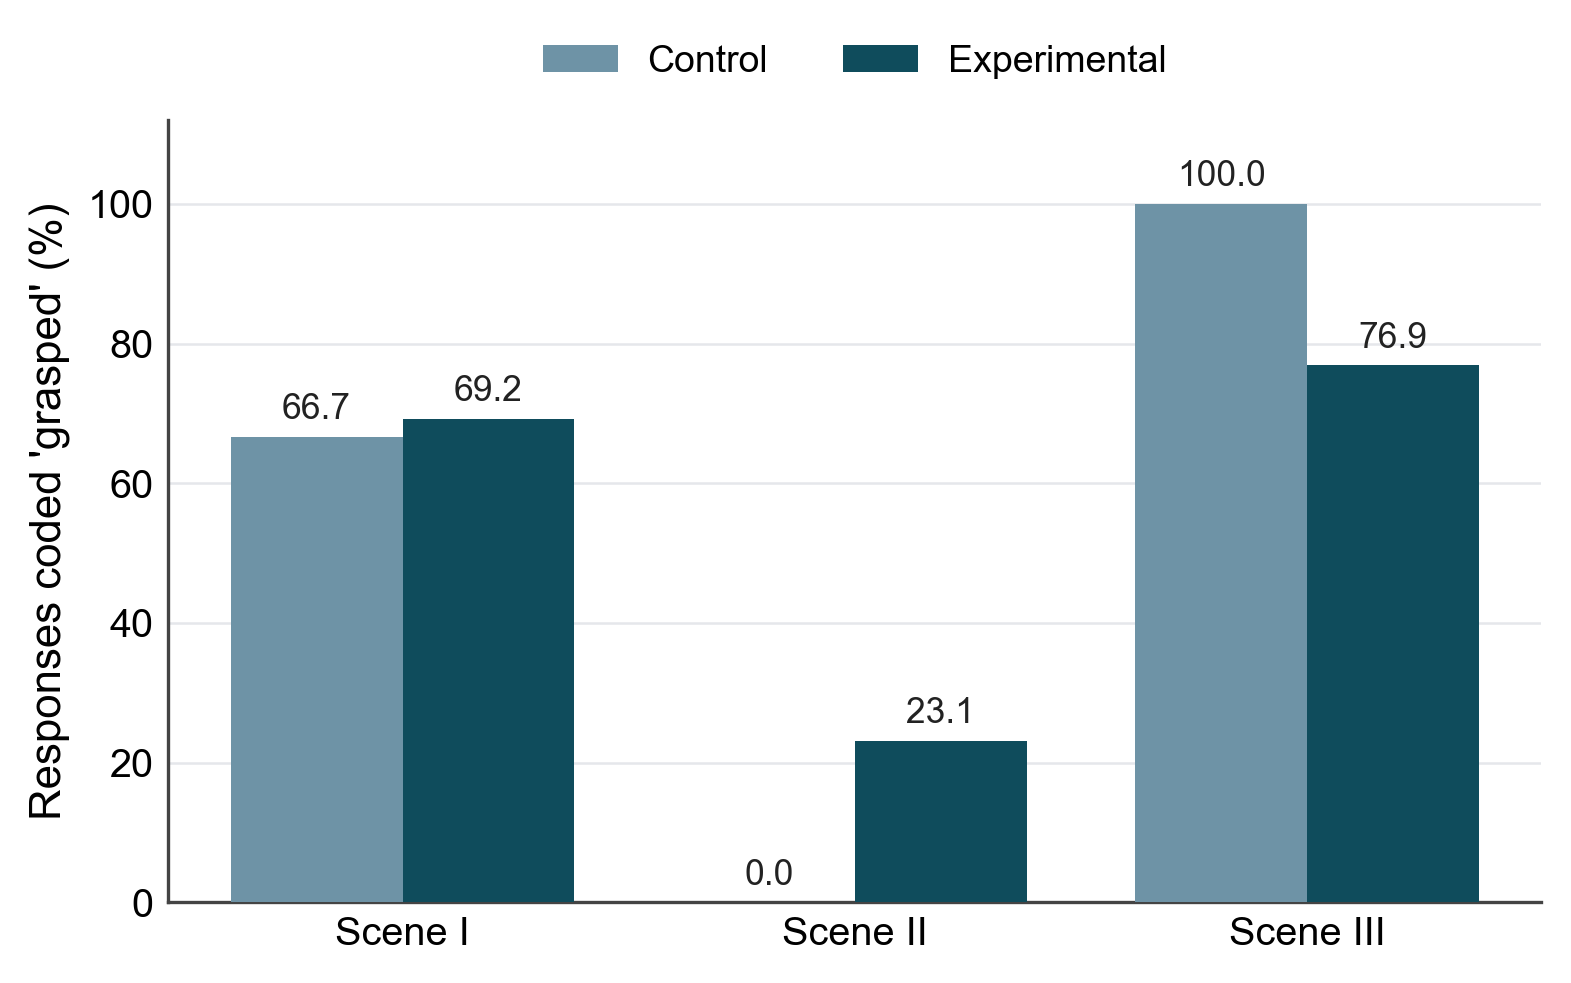
\includegraphics[width=\textwidth]{figures/results/F1_grasped_by_condition_scene.png}
\caption[Comprensione strutturale per condizione e scena]{Percentuale di risposte codificate \emph{grasped} per condizione, per ciascuna scena. La direzione della differenza tra le due condizioni non è la stessa nelle tre scene.}
\label{fig:grasped}
\end{figure}

\begin{figure}[tbp]
\centering
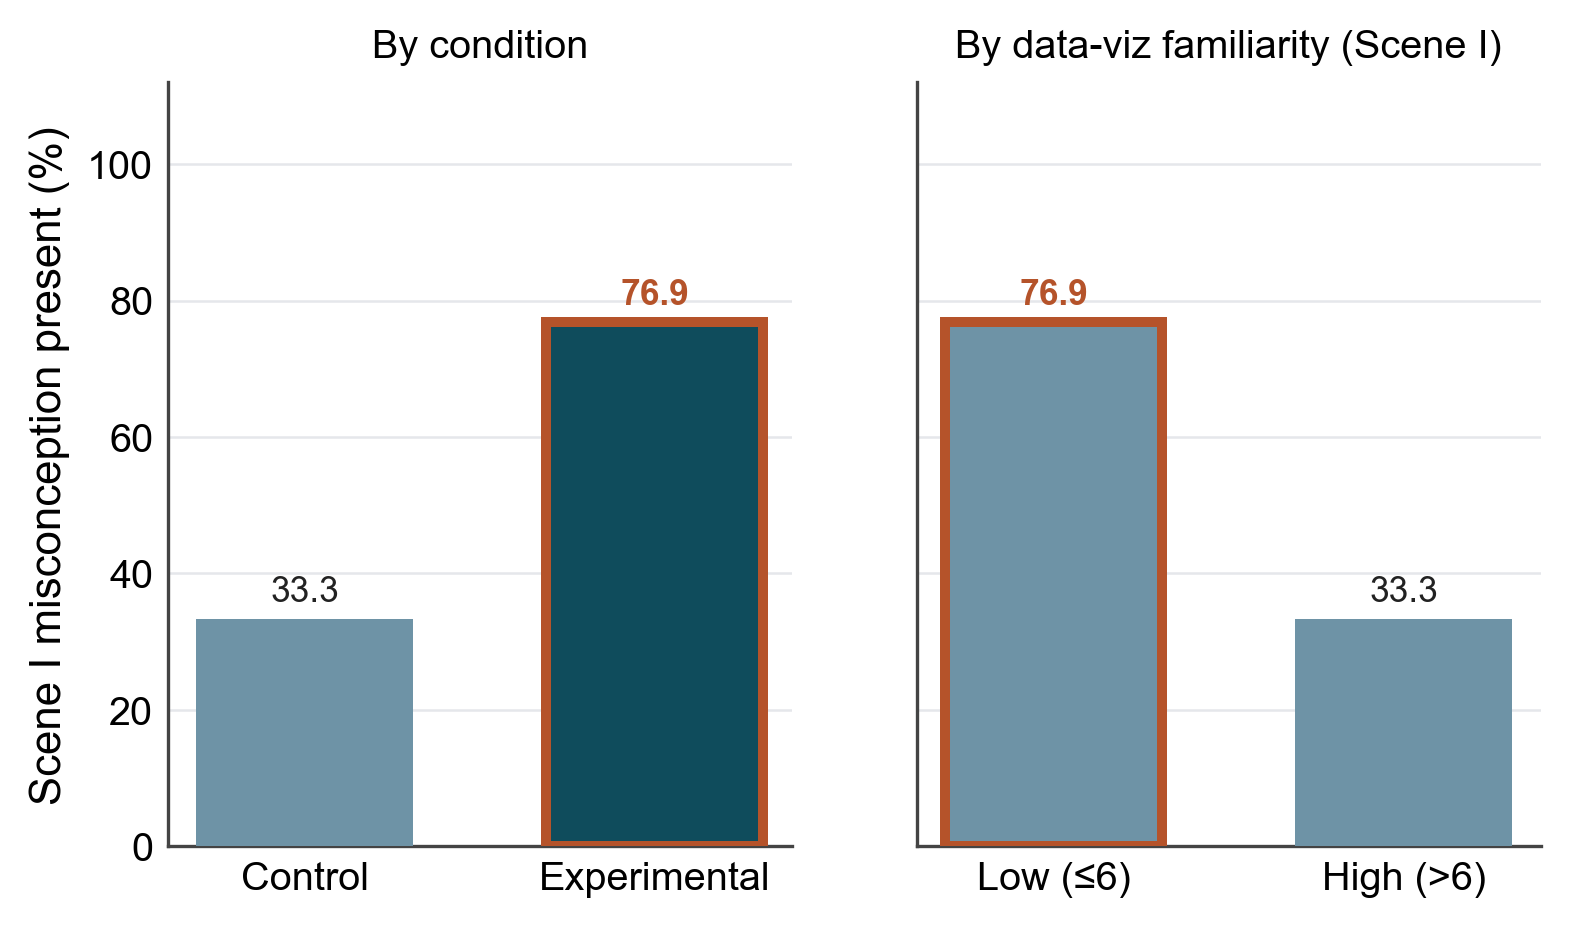
\includegraphics[width=\textwidth]{figures/results/F2_misconception.png}
\caption[L'errore sulla funzione di corrente, per condizione e per familiarità]{Presenza dell'errore S1-MISC-INT nella Scena~I. A sinistra: per condizione. A destra: per familiarità auto-valutata con le visualizzazioni di dati. I due pannelli sono in parte confusi (vedi \S\ref{sec:res-misconception}).}
\label{fig:misconception}
\end{figure}

\begin{figure}[tbp]
\centering
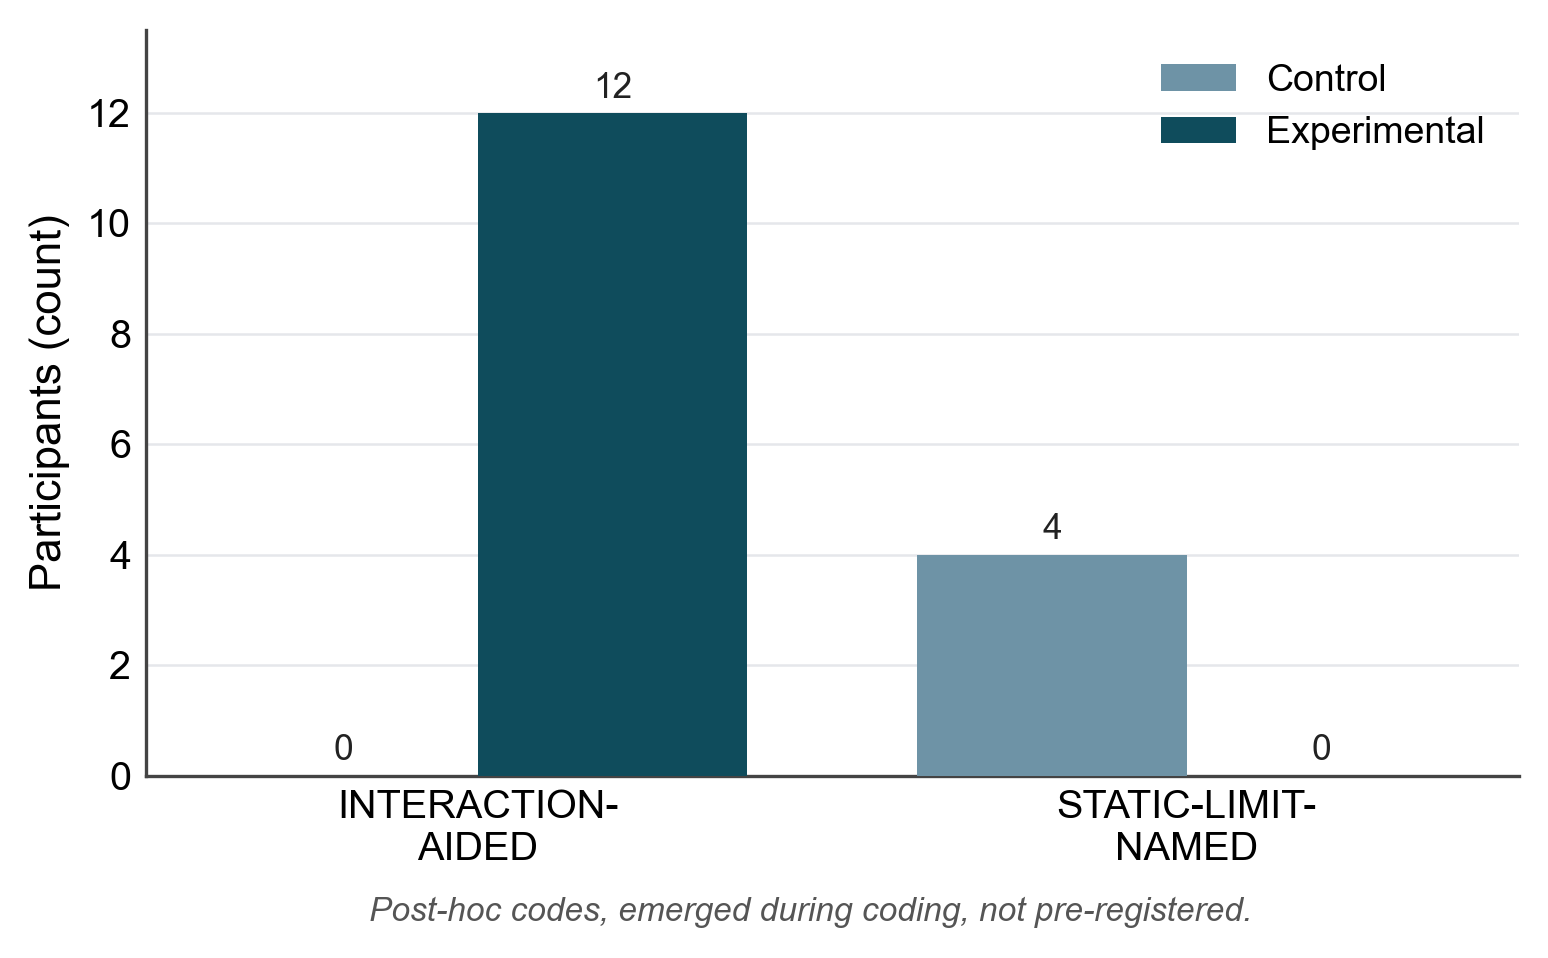
\includegraphics[width=\textwidth]{figures/results/F3_emergent_mechanism.png}
\caption[Codici emergenti ricorrenti per condizione]{I tre codici emergenti ricorrenti per condizione. I primi due sono immagini speculari l'uno dell'altro; il terzo va contro la condizione sperimentale. Codici post-hoc emersi durante la codifica; non parte della griglia definita a priori.}
\label{fig:emergent}
\end{figure}

\begin{figure}[tbp]
\centering
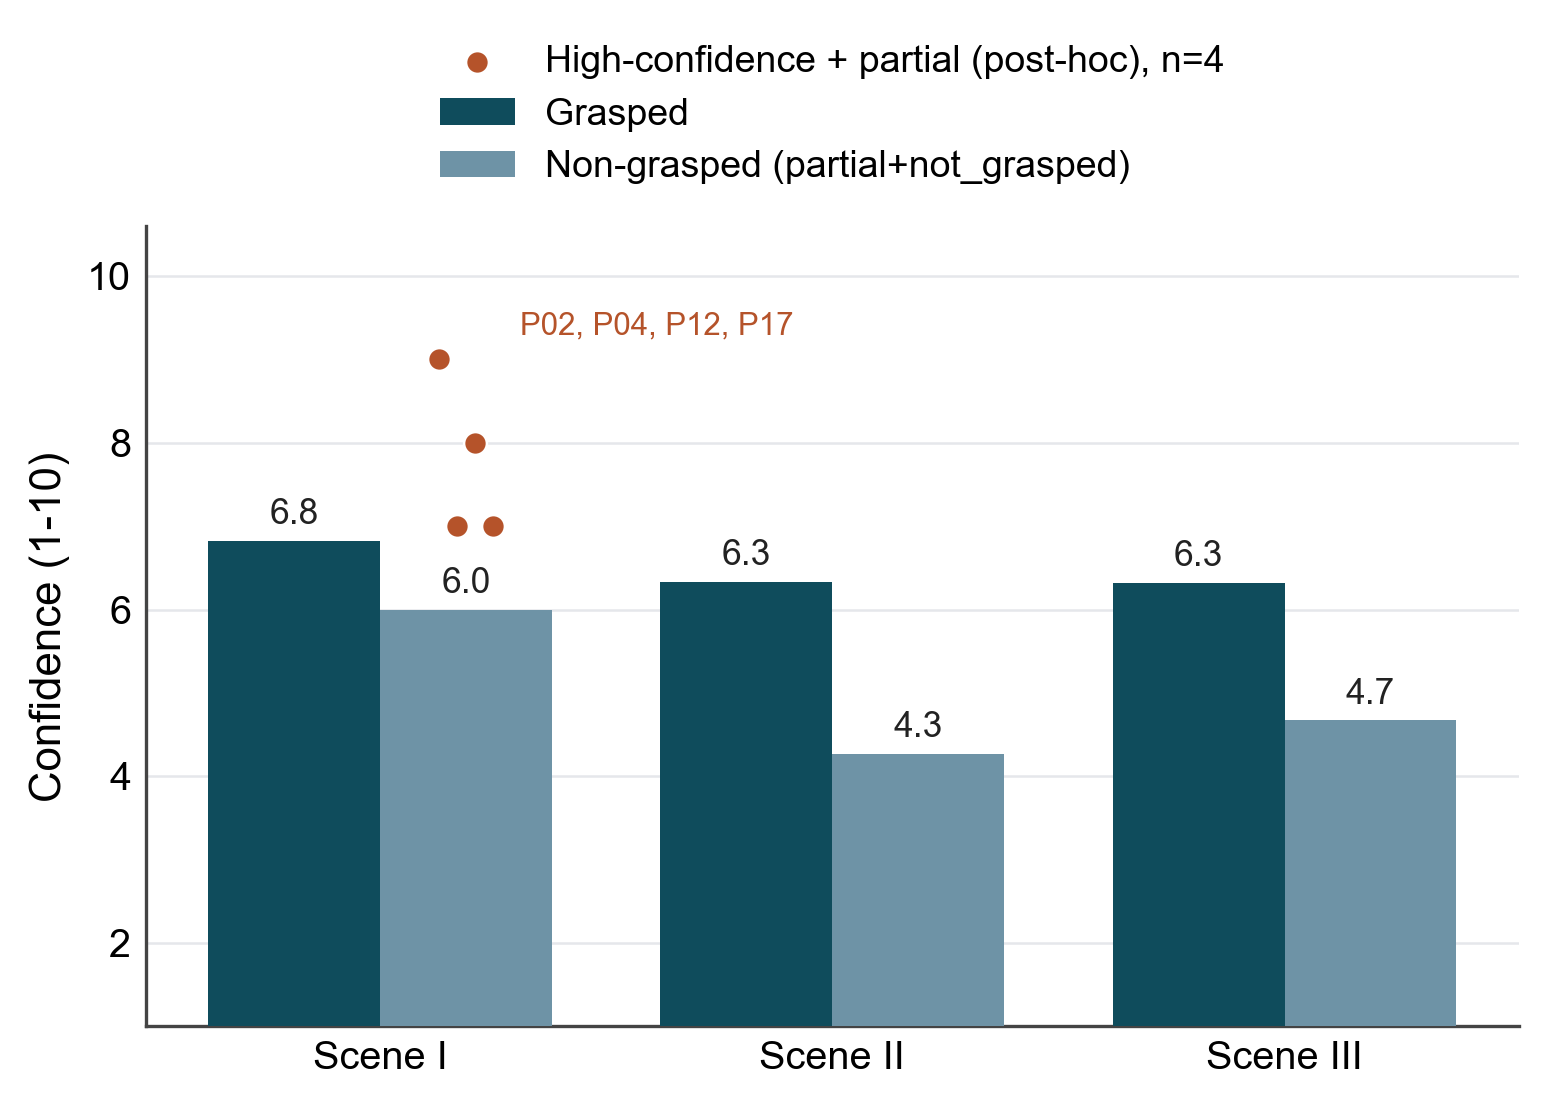
\includegraphics[width=\textwidth]{figures/results/F4_confidence_by_correctness.png}
\caption[Fiducia per correttezza e scena]{Fiducia media delle risposte grasped contro non grasped (partial e not-grasped accorpate), per scena. I quattro punti evidenziati segnano i partecipanti della Scena~I con fiducia $\geq 7$ e verdetto partial (lettura post-hoc; vedi \S\ref{sec:res-confidence}).}
\label{fig:confidence}
\end{figure}

\begin{figure}[tbp]
\centering
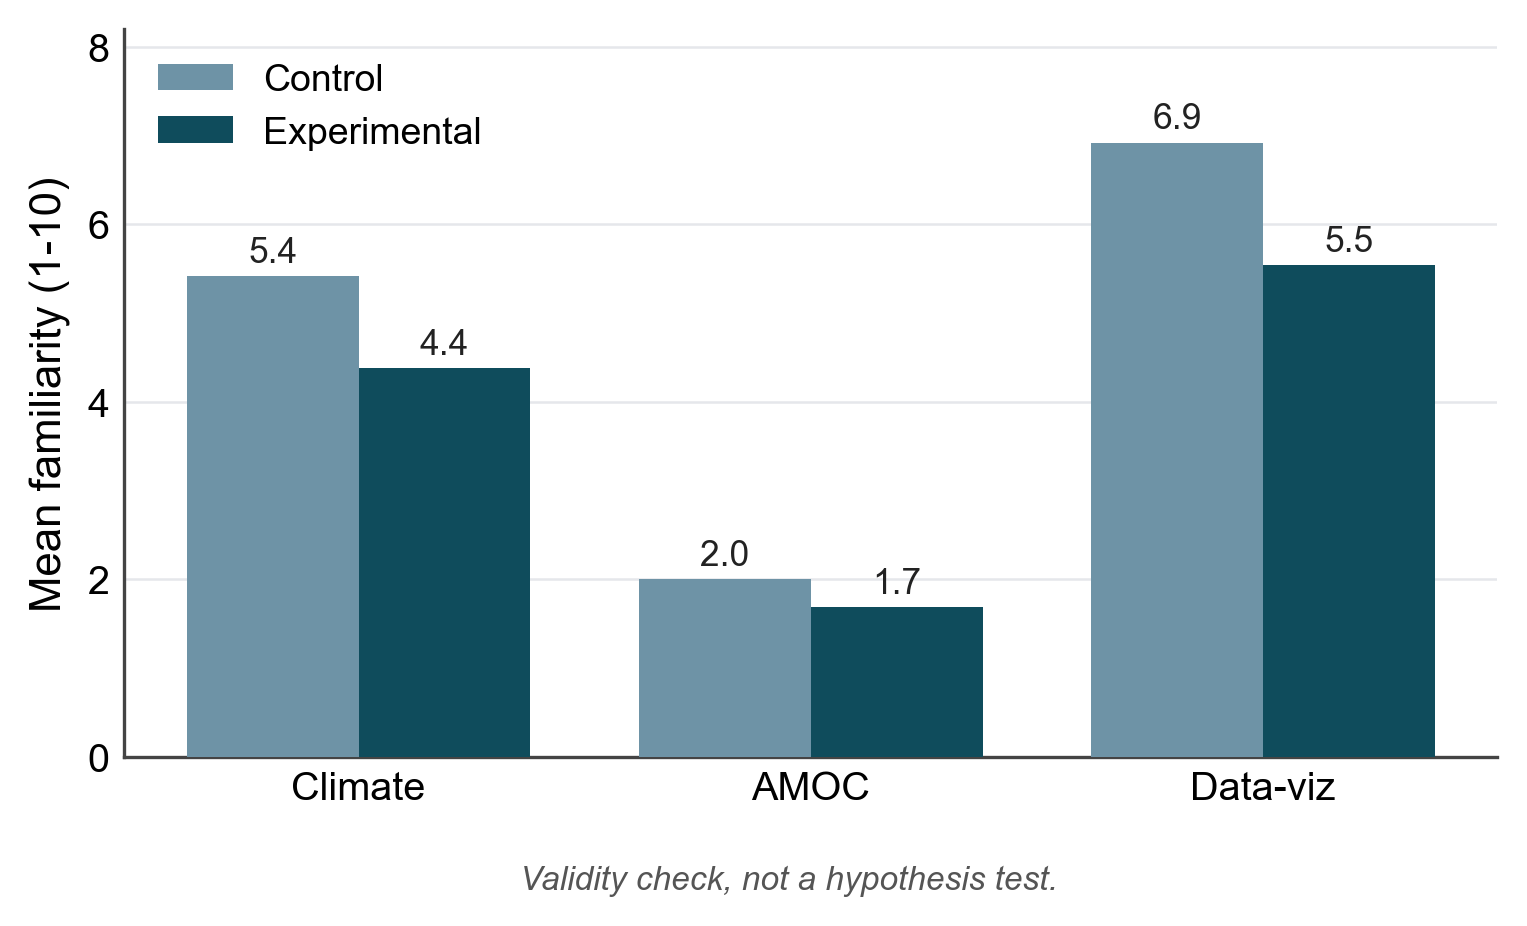
\includegraphics[width=\textwidth]{figures/results/S1_balance_familiarity.png}
\caption[Controllo di equilibrio: familiarità per condizione]{Familiarità media auto-valutata sulle tre misure, per condizione. Un controllo di equivalenza tra gruppi, non un test di ipotesi.}
\label{fig:balance}
\end{figure}

\begin{figure}[tbp]
\centering
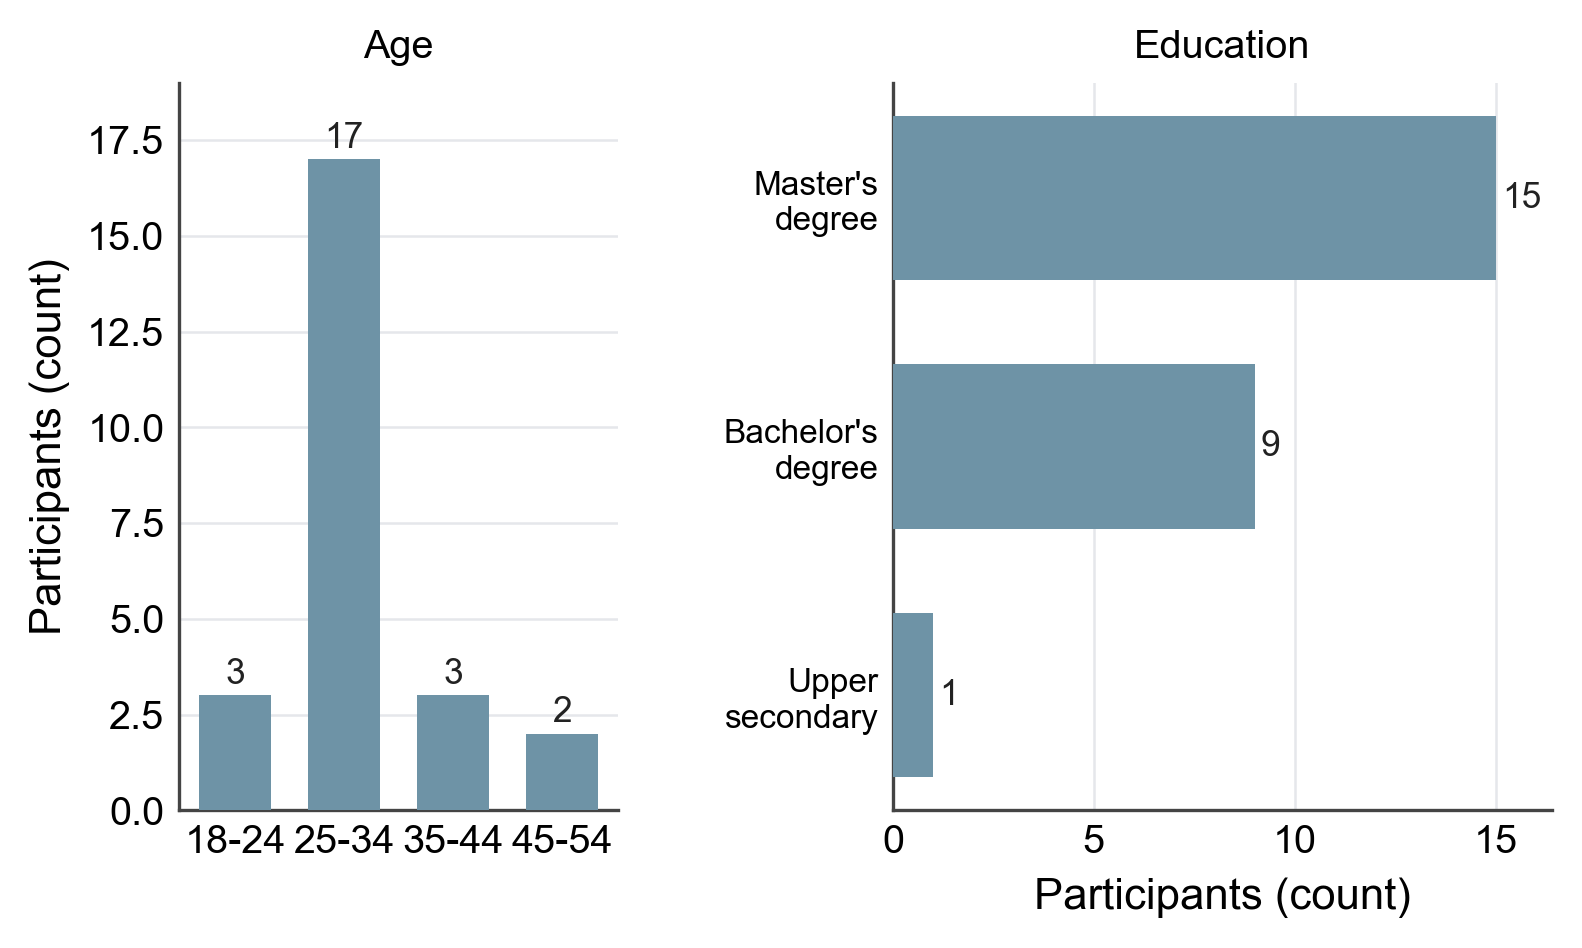
\includegraphics[width=\textwidth]{figures/results/S2_demographics.png}
\caption[Dati demografici del campione]{Distribuzione della fascia d'età e del titolo di studio più elevato nel campione.}
\label{fig:demographics}
\end{figure}

\begin{figure}[tbp]
\centering
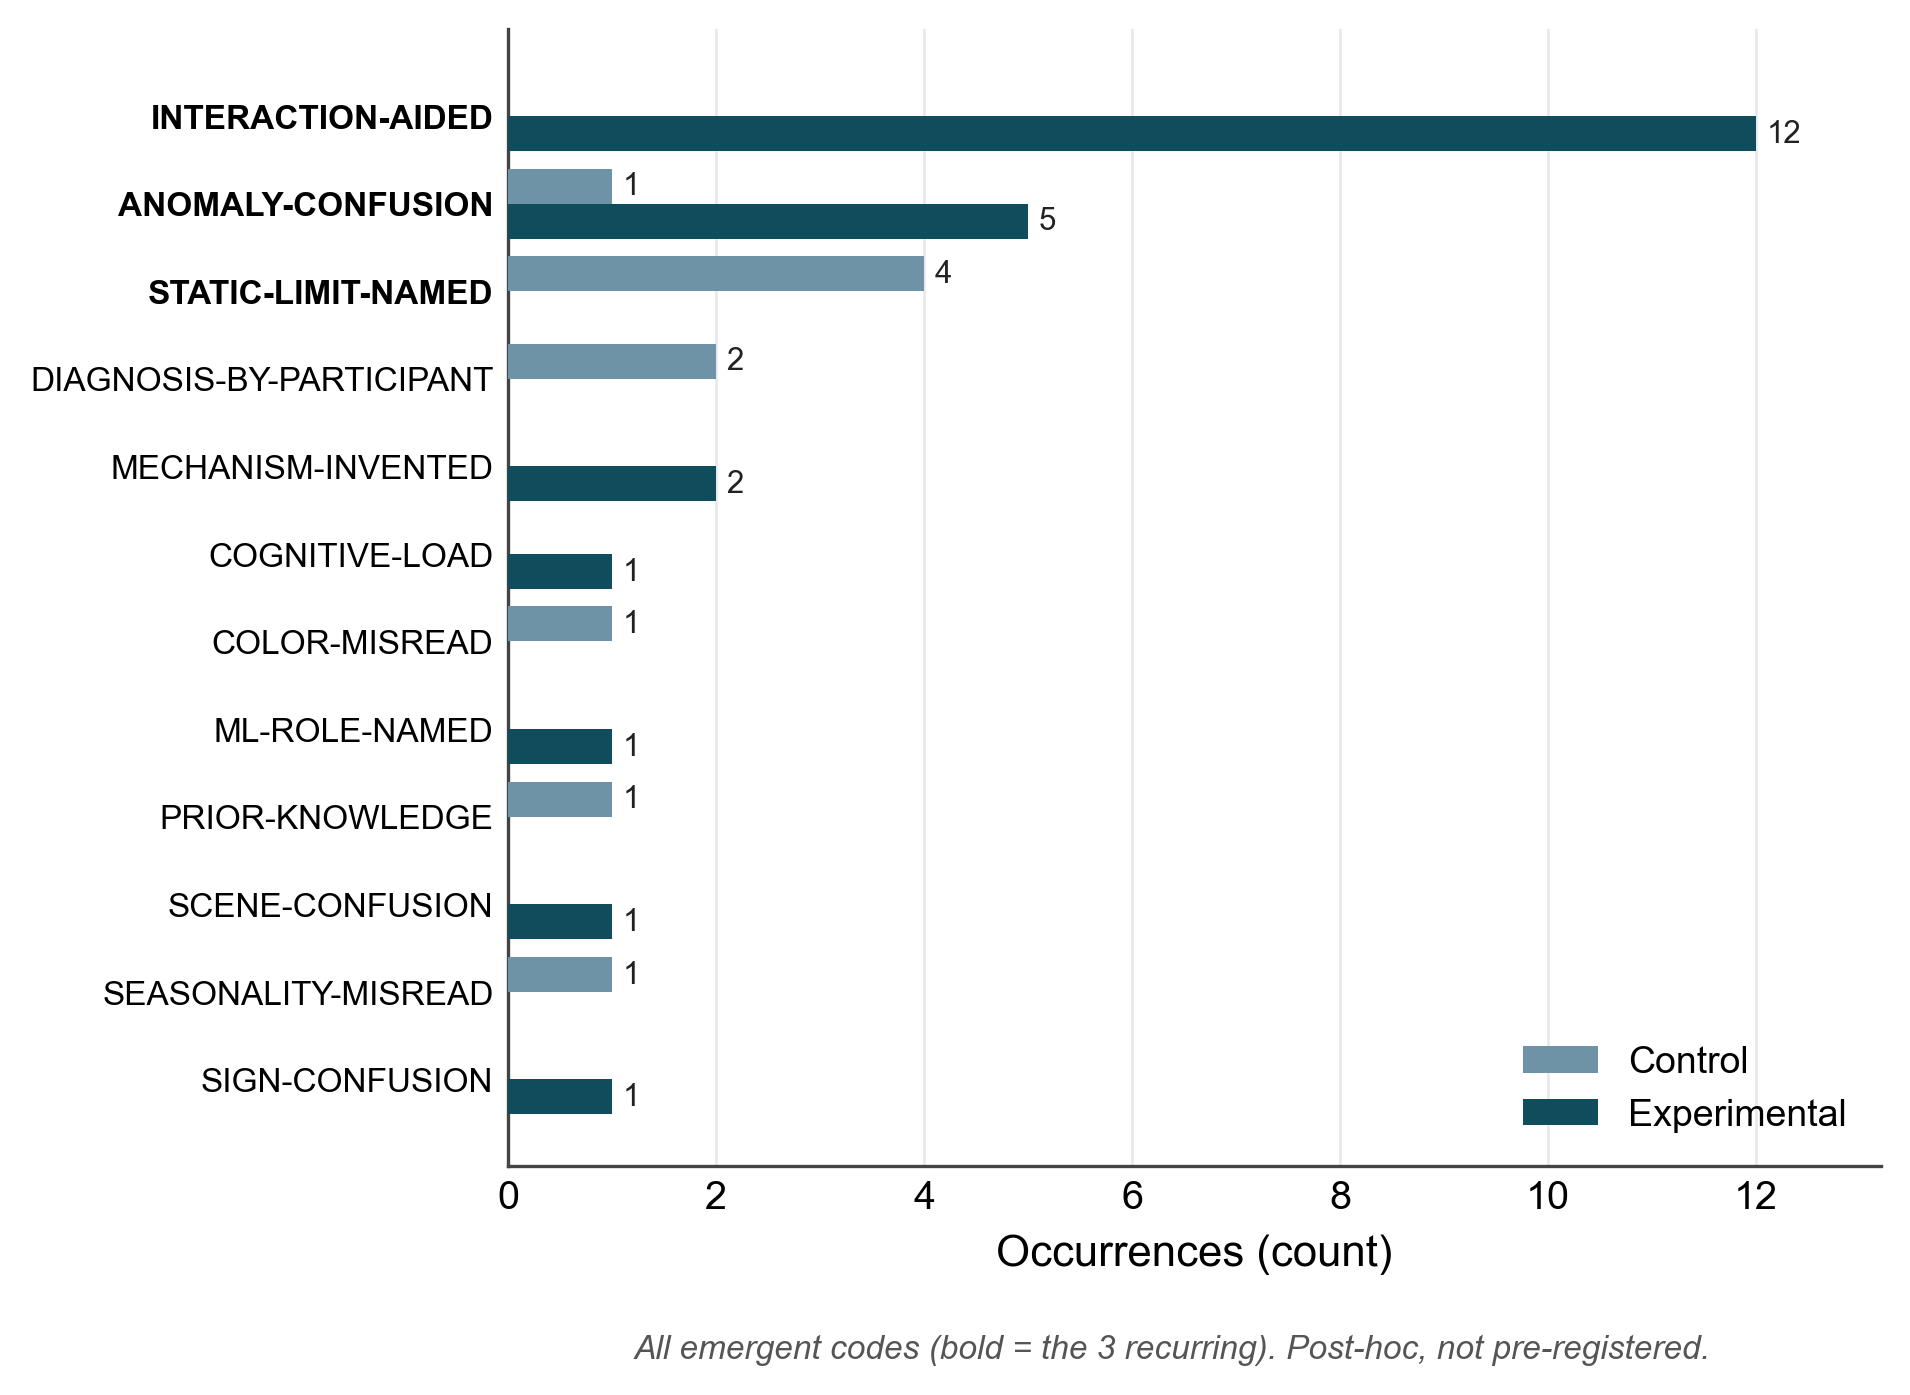
\includegraphics[width=\textwidth]{figures/results/S4_emergent_all_codes.png}
\caption[Tutti i codici emergenti per condizione]{L'elenco completo dei codici emergenti per condizione. Il grassetto segna i tre codici ricorrenti. Tutti sono post-hoc e non facevano parte della griglia definita a priori.}
\label{fig:emergent-full}
\end{figure}

% =========================================================================
% CAPITOLO 10 — DISCUSSIONE
% =========================================================================

\chapter{Discussione}
\label{ch:discussion}

\noindent
{\rmfamily\itshape
\begin{tabular}[t]{@{}l@{\hspace{0.3cm}}p{12.5cm}@{}}
\textls[50]{\textbf{Trattati:}} &
\textls[50]{Interpretazione · Aspettative riviste · Meccanismo e condizioni al contorno ·
Implicazioni teoriche, pratiche e di sostenibilità · Ciò che lo studio può e non può affermare}
\end{tabular}
}

\vspace{0.5cm}

Il Capitolo~\ref{ch:results} ha riportato ciò che mostrano le risposte codificate; questo capitolo chiede cosa significhino. Legge i risultati rispetto alle aspettative che hanno inquadrato lo studio con utenti, e indica dove l'evidenza sostiene la tesi, dove la complica e dove non può pronunciarsi. Con venticinque partecipanti, lo studio non può dimostrare un'affermazione generale; ciò che può fare è mostrare se i pattern che è stato costruito per cercare compaiano davvero --- e il risultato più utile di un primo studio spesso non è una conferma ma una comprensione più affinata di dove l'approccio aiuta e perché.

% -------------------------------------------------------------------------
\section{Rileggere le aspettative alla luce dello studio realizzato}
\label{sec:disc-translate}

Le aspettative per la valutazione, E3.1 ed E3.2, sono state scritte presto, per un disegno che poi è cambiato: tre condizioni di crescente ricchezza esperienziale e un protocollo think-aloud sono diventate due condizioni e un questionario scritto auto-somministrato (Capitolo~\ref{ch:userstudy}). Vanno quindi lette in forma tradotta. E3.1 --- che una maggiore ricchezza esperienziale si sarebbe mostrata in \emph{come} i partecipanti articolano la propria comprensione anziché in un punteggio di comprensione --- è letta come un confronto tra le due condizioni. E3.2 --- che le codifiche percettive avrebbero prodotto interpretazioni che il protocollo poteva far emergere, corrispondenti o meno alla lettura intesa --- è letta come riferita a ciò che le risposte scritte rivelano.

Questa traduzione è un limite, ed è enunciata come tale; ma non indebolisce le aspettative, perché E3.1 era prudente esattamente nel modo che si è rivelato importante. Non prevedeva che la condizione esperienziale aumentasse la comprensione; prevedeva una differenza nell'articolazione, non nel punteggio --- che è precisamente ciò che i risultati mostrano.

% -------------------------------------------------------------------------
\section{E3.1: l'aspettativa prudente regge, quella ingenua no}
\label{sec:disc-e31}

Il singolo risultato più netto è che la condizione esperienziale non ha prodotto un guadagno uniforme di comprensione. Nelle tre scene la direzione della differenza non era la stessa (Figura~\ref{fig:grasped}): pari nella Scena~I, a favore della condizione sperimentale nella Scena~II, a favore del controllo nella Scena~III. Uno studio che si fosse aspettato che la presentazione esperienziale alzasse ovunque la comprensione sarebbe messo in imbarazzo da questo pattern. Il presente studio no, perché non se lo è mai aspettato.

Se l'aspettativa fosse stata quella ingenua --- che una rappresentazione più ricca e in movimento produca semplicemente una comprensione migliore --- i dati l'avrebbero rifiutata. Ciò che è cambiato con la ricchezza esperienziale non è stato il punteggio di comprensione ma il carattere della comprensione, e dove essa fosse affatto raggiungibile: esattamente la forma di E3.1. L'avvertimento che le visualizzazioni animate possono apparire efficaci solo perché introducono di nascosto informazione che la versione statica non ha \parencite{tversky2002} è il motivo per cui le due condizioni sono state allineate per provenienza, inquadramento e unità di misura, con la versione esperienziale che aggiunge solo la dimensione temporale che lo studio si propone di esaminare. Il confronto piatto nella Scena~I è onesto anziché deludente.

% -------------------------------------------------------------------------
\section{Dove vive la differenza, e perché}
\label{sec:disc-mechanism}

Se l'effetto non è un aumento uniforme, la domanda interessante è dove compaia e perché.

La Scena~II riguarda la ricorrenza: se il sistema ripassi per stati che ha già occupato. Uno scatter immobile non può mostrarlo, perché senza un ordinamento nel tempo non c'è nulla che riveli un ritorno. I risultati corrispondono esattamente. Nessun partecipante di controllo è stato codificato come avente colto la ricorrenza, contro circa un quarto del gruppo sperimentale, con in aumento anche la comprensione parziale (Capitolo~\ref{ch:results}). Il meccanismo non è dedotto; lo enunciano i partecipanti stessi. Ogni risposta \textsc{Interaction-aided} --- che attribuisce la comprensione al mettere in pausa, riavvolgere o isolare parte del display --- veniva dalla condizione sperimentale, e ogni risposta \textsc{Static-limit-named} --- che nomina l'assenza di un ordinamento temporale come la ragione per cui la ricorrenza non poteva essere giudicata --- veniva dal controllo (Figura~\ref{fig:emergent}): le due facce della stessa affermazione, dette da lati opposti del disegno.

Un terzo codice emergente va contro la condizione esperienziale, ed è riportato qui per la stessa ragione per cui lo è l'inversione della Scena~III. \textsc{Anomaly-confusion}, che segna la difficoltà con la codifica usuale/insolito, è comparso cinque volte nella condizione sperimentale contro una nel controllo (\S\ref{sec:res-emergent}). Il principio~P3 assegna l'anomalia a texture e agitazione, sul presupposto che l'irregolarità attiri l'attenzione senza una legenda \parencite{bertin1983, ware2021}. Queste risposte suggeriscono che attirare l'attenzione non è lo stesso che trasmettere significato: i partecipanti notavano il disturbo e non sapevano dire cosa significasse. La salienza pre-attentiva pare sufficiente per il rilevamento e insufficiente per l'interpretazione --- un limite di P3 così come enunciato, e un obiettivo specifico di revisione.

La Scena~III è la prova che rende tutto questo credibile, perché va nell'altro verso. Qui la condizione di controllo ha fatto meglio, raggiungendo ogni partecipante contro circa tre quarti del gruppo sperimentale. La ragione è istruttiva anziché imbarazzante. La Scena~III chiede se l'accordo tra tre modelli cambi nel tempo, e una figura statica mostra l'intera serie temporale in una volta, dispiegando la convergenza da leggere in un'unica vista. La versione esperienziale chiede al partecipante di costruire quella stessa lettura muovendosi tra i controlli, e alcuni non l'hanno completata. Una seconda spiegazione non può essere separata dalla prima con questo disegno: la Scena~III veniva per ultima per ogni partecipante, e la versione esperienziale chiede attenzione sostenuta proprio dove l'attenzione è meno probabile che resti. L'ordine fisso delle scene (\S\ref{sec:eval-limitations}) fa sì che i due resoconti siano confusi, e lo studio non può decidere tra essi. Sotto entrambe le letture, la lezione non è che la forma esperienziale abbia fallito. È che la presentazione esperienziale non è gratuita. Aiuta di più dove la struttura è invisibile in una figura immobile, come nella Scena~II, e può costare attenzione dove una figura statica già la dispiega con chiarezza, come nella Scena~III. Un approccio che ammette questo è più forte di uno che rivendica un vantaggio uniforme, perché può dire \emph{dove} si applica.

% -------------------------------------------------------------------------
\section{E3.2 e l'errore sulla funzione di corrente}
\label{sec:disc-e32}

Il risultato più sostanziale dello studio è una lettura errata, ed E3.2 anticipava esattamente questo genere di cosa: che i non specialisti avrebbero interpretato la rappresentazione in modi che valeva la pena far emergere, che l'interpretazione corrispondesse o no a quella intesa. Quattordici partecipanti su venticinque hanno letto l'altezza della curva della funzione di corrente nella Scena~I come la velocità dell'acqua, anziché come il trasporto cumulato che rappresenta (Capitolo~\ref{ch:results}). La curva invita quella lettura. La sua altezza è la cosa più saliente sul display, e l'altezza si legge naturalmente come quantità o velocità; la lettura corretta, che direzione e intensità vivono nella pendenza della curva, richiede un'inferenza che un non specialista non fa spontaneamente.

Questa lettura errata non è specifica di un dominio, e il Capitolo~\ref{ch:literature} la nomina già. La funzione di corrente è un integrale cumulato del trasporto, la sua pendenza il tasso locale (Equazione~\ref{eq:velocity}); leggere la sua altezza come velocità è la confusione stock--flusso che \textcite{sterman2008} e \textcite{cronin2009} documentano in adulti matematicamente competenti. Lo studio aggiunge che la confusione sopravvive alla traduzione in un dominio e in un idioma diversi: i partecipanti hanno incontrato una curva oceanografica anziché un diagramma stock-e-flusso e hanno fatto la stessa sostituzione --- un limite noto dell'architettura cognitiva che riappare esattamente dove il filone delle scienze cognitive prevedeva, trasformando il risultato della Scena~I da anomalia in conferma.

Due ulteriori pattern trasformano questo da errore in risultato. Il primo è che l'errore era più frequente nella condizione sperimentale, non meno (Figura~\ref{fig:misconception}). A prima vista questo contraddice la tesi. Non è così, una volta affiancato il secondo pattern: l'errore calava nettamente con la familiarità con le visualizzazioni di dati, da circa tre quarti dei partecipanti meno familiari a un terzo dei più familiari. Il display esperienziale mostra particelle in movimento, e le particelle in movimento rendono la lettura di velocità più immediata, non meno. La ricchezza percettiva che ha aiutato i partecipanti a vedere la ricorrenza nella Scena~II qui lavora contro di loro, rendendo la lettura seducente più facile proprio per chi ha meno strumenti per correggerla. Questo non è tanto un fallimento dell'approccio quanto una lezione su di esso: la salienza percettiva è potente in entrambe le direzioni, e una rappresentazione che rende vivida una struttura può rendere vivida anche una lettura errata adiacente.

Che le due condizioni differissero anche nella familiarità media con le visualizzazioni di dati significa che condizione e familiarità non possono essere pienamente separate a questa dimensione campionaria (Capitolo~\ref{ch:results}), perciò la lettura congiunta è esplorativa. La direzione è comunque abbastanza chiara da portare una conseguenza di design, ripresa nel Capitolo~\ref{ch:conclusion}: un'iterazione futura deve rendere percepibile la natura cumulata della curva anziché lasciare che sia l'osservatore a fornirla.

L'errore dà anche a E3.2 il suo spigolo di sicurezza-ma-errore. \textcite{fischer2020} descrivono casi in cui un'alta fiducia si attacca a una lettura errata, e la Scena~I ne contiene: quattro partecipanti hanno valutato la propria fiducia a sette o più pur leggendo la curva solo parzialmente, ciascuno portando l'errore sulla funzione di corrente (Figura~\ref{fig:confidence}). La fiducia, in questa scena, non segue la comprensione. Le persone più sicure della propria lettura erano tra quelle che avevano letto male lo strumento, che è precisamente il motivo per cui lo studio ha tenuto separate comprensione percepita e dimostrata anziché lasciare che una valutazione di fiducia facesse le veci di una presa.

% -------------------------------------------------------------------------
\section{Ciò che lo studio non può affermare}
\label{sec:disc-limits}

Tre limiti vincolano queste letture, e nominarli è parte dell'argomentazione anziché una scusa aggiunta a essa.

Il campione è piccolo ed è stato reclutato per convenienza, perciò nulla qui si generalizza a una popolazione e i test esplorativi non portano peso inferenziale. Il confronto della Scena~III, dove il controllo ha fatto meglio, è reale quanto quello della Scena~II, e lo studio riporta entrambi anziché il solo lusinghiero. Il confondimento tra condizione e familiarità con le visualizzazioni di dati significa che i due pannelli del risultato sull'errore non sono indipendenti: il risultato è una direzione da testare, non un effetto accertato. E la codifica poggia su un singolo ricercatore supportato da un primo passaggio automatico, perciò non può essere riportata alcuna affidabilità tra codificatori (Capitolo~\ref{ch:userstudy}). Nessuno è fatale a un primo studio; ciascuno è una ragione perché il prossimo sia più ampio, bilanciato sulla familiarità pregressa, codificato in modo indipendente e controbilanciato sull'ordine delle scene.

% -------------------------------------------------------------------------
\section{Implicazioni}
\label{sec:disc-implications}

\paragraph{Teoriche.} Lo studio fornisce un caso in cui la confusione stock--flusso di \textcite{sterman2008} riappare in un idioma visivo scientifico anziché in un diagramma da manuale (\S\ref{sec:disc-e32}), e uno in cui il principio di equivalenza di \textcite{tversky2002} fa un lavoro reale: con provenienza, inquadramento e unità mantenuti costanti e solo la dimensione temporale aggiunta, il vantaggio dell'animazione non compare in modo uniforme. Qualifica anche la letteratura sull'incertezza animata \parencite{hullman2015hops, kale2019hops}: la Scena~III ha animato l'incertezza e non ha superato la baseline statica, il che suggerisce che il beneficio possa dipendere da se l'alternativa statica offra già una vista dell'intera serie.

\paragraph{Pratiche.} Per chiunque progetti una rappresentazione di un sistema invisibile, il risultato è una regola di selezione, non un avallo: il movimento merita il suo costo dove la struttura è temporale e non disponibile in una figura immobile, e aggiunge carico attentivo senza comprensione dove una figura statica la dispiega già. La salienza va verificata in entrambe le direzioni: il campo di particelle che ha reso visibile il contro-flusso nella Scena~I ha reso anche più disponibile la lettura errata di velocità, soprattutto per chi era meno attrezzato a correggerla.

\paragraph{Sostenibilità e comunicazione.} Che la comprensione non segua la chiarezza percepita estende \textcite{hegarty2012} a un formato esperienziale, e riguarda come il materiale sul clima è preparato per il pubblico non specialista: un artefatto valutato sulla sola preferenza o sul solo coinvolgimento può essere ottimizzato nella direzione sbagliata. La memoria di lavoro è il vincolo stringente \parencite{sweller1988}, e una rappresentazione che la spende in decorazione anziché in struttura la spende male.

% -------------------------------------------------------------------------
\section{Cosa significa per H-A e H-B}
\label{sec:disc-umbrella}

Le ipotesi ombrello hanno inquadrato l'intera indagine: che le rappresentazioni convenzionali siano percettivamente subottimali per i non specialisti perché trattano la complessità come un oggetto da leggere anziché una dinamica da abitare (H-A), e che le rappresentazioni esperienziali derivate dal machine learning possano sostenere la comprensione rendendo la struttura percettivamente disponibile (H-B). Venticinque partecipanti non possono dimostrare nessuna delle due. Entrambe trovano il loro sostegno più netto nella Scena~II, dove la rappresentazione statica ha lasciato la ricorrenza semplicemente irraggiungibile e i partecipanti l'hanno detto con parole proprie, e in coloro che hanno attribuito la propria comprensione all'agire sul display.

Il contributo più prezioso è il confine che lo studio traccia attorno a H-B, esposto nella \S\ref{sec:disc-mechanism} e nella \S\ref{sec:disc-implications}: la presentazione esperienziale non è uniformemente migliore, e il suo potere percettivo può approfondire una lettura errata con la stessa facilità di una corretta. La tesi emerge non come dimostrata ma come affinata --- la domanda non è più se la rappresentazione esperienziale aiuti, ma per quali strutture, per quali osservatori e a quale costo percettivo.

% =========================================================================
% CAPITOLO 11 — CONCLUSIONE
% =========================================================================

\chapter{Conclusione}
\label{ch:conclusion}

\noindent
{\rmfamily\itshape
\begin{tabular}[t]{@{}l@{\hspace{0.3cm}}p{12.5cm}@{}}
\textls[50]{\textbf{Trattati:}} &
\textls[50]{Sintesi · Risposta alla domanda di ricerca · Contributo metodologico ·
Trasferibilità · Lavori futuri e implicazioni di design}
\end{tabular}
}

\vspace{0.5cm}

Questa tesi è iniziata con una domanda apparentemente semplice: come si rende comprensibile un sistema quando non lo si può vedere? E con una seconda domanda che dà alla prima un metodo: in che misura una rappresentazione esperienziale alimentata dal machine learning può sostenere il lavoro della comprensione?

La Atlantic Meridional Overturning Circulation è servita da caso, ma la domanda non è chiaramente mai stata solo sull'AMOC. Riguardava la più ampia classe di sistemi --- invisibili, dinamici, che si dispiegano su scale temporali più lunghe di una vita umana --- il cui comportamento conta e la cui struttura resiste ai modi convenzionali in cui la disegniamo. Questo capitolo conclusivo riunisce l'arco, enuncia ciò che il lavoro contribuisce e segna le strade che apre.

% -------------------------------------------------------------------------
\section{Rispondere alla domanda di ricerca}
\label{sec:concl-answer}

Le tre fasi --- rilevare, tradurre, valutare --- hanno fatto tipi diversi di affermazioni (Capitolo~\ref{ch:rqs}) e si sono quindi chiuse in modo diverso; questo è parte della risposta.

La fase di \emph{rilevamento} (RQ1) ha prodotto affermazioni verificabili rispetto ai dati --- e hanno retto: la struttura verticale dell'AMOC si riduce a due modi che spiegano quasi il novantotto per cento della varianza, un autoencoder ha confermato che lo spazio ridotto è abbastanza piatto da fungere da sistema di coordinate (H2), e l'analisi di preallarme ha restituito un rigoroso risultato nullo (H3). Questi sono i risultati più solidi della tesi: affermazioni su un dataset.

La fase di \emph{traduzione} (RQ2) chiedeva solo che l'artefatto esistesse e funzionasse. \emph{Living Atlantic} lo fa: gira e mantiene le sue due condizioni allineate per provenienza, inquadramento e unità di misura attraverso un bundle di dati e una ricostruzione condivisi, differendo solo nella dimensione temporale oggetto di studio (Capitolo~\ref{ch:translate}).

La fase di \emph{valutazione} (RQ3) è stata più prudente, chiedendo come i partecipanti esprimessero la comprensione anziché se ottenessero punteggi più alti. La presentazione esperienziale non ha migliorato la comprensione in ogni caso; ha cambiato come i partecipanti comprendevano il sistema e quali aspetti sapevano identificare (Capitolo~\ref{ch:discussion}). Le due ipotesi ricevono quindi un sostegno direzionale anziché una prova: H-A (le rappresentazioni convenzionali possono lasciare strutture inaccessibili ai non specialisti) e H-B (la rappresentazione esperienziale può renderle più accessibili) trovano il loro sostegno più netto nella scena della ricorrenza, dove nessun partecipante della condizione statica ha identificato la struttura ricorrente mentre diversi hanno nominato ciò che mancava; il sostegno è più debole dove una struttura è già visibile in una figura immobile.

La risposta onesta non è che la visualizzazione esperienziale funzioni, ma che funziona \emph{condizionatamente}: la sua utilità dipende da ciò che va compreso, aiutando dove un pattern è difficile da vedere e offrendo meno dove è già visibile.

Come il Capitolo~\ref{ch:introduction} anticipava, il contributo principale è metodologico, non oceanografico: un framework trasferibile, qui evidenziato attraverso l'AMOC, per trasformare un sistema complesso e difficile da osservare in una rappresentazione testabile, con ciascuna fase tenuta al proprio standard di evidenza --- verifica, costruzione e confronto esplorativo.

Due ulteriori contributi gli stanno accanto. Empiricamente, lo studio ha fatto emergere un errore ricorrente: più della metà dei partecipanti ha letto l'altezza della curva cumulata della funzione di corrente come velocità locale, una lettura errata che la ricchezza aggiunta non ha ridotto e che era più rara tra i partecipanti più esperti --- inatteso, e da testare su larga scala. Materialmente, \emph{Living Atlantic} resta un oggetto di design riproducibile costruito sulla provenienza condivisa, utilizzabile in studi futuri anziché solo come dimostrazione.

Insieme, questi collocano la tesi come un ponte tra dati scientifici e comprensione umana anziché come un contributo all'oceanografia, allineata come esposto nella \S\ref{sec:contribution} con l'\textbf{SDG~13} (educazione e consapevolezza climatica), l'\textbf{SDG~4} e l'\textbf{SDG~14}.

% -------------------------------------------------------------------------
\section{Lavori futuri}
\label{sec:concl-future}

Il passo successivo più chiaro discende dai risultati. Il piccolo campione di convenienza e la differenza di alfabetizzazione visiva pregressa tra i gruppi limitano le conclusioni; uno studio più ampio, bilanciato su quell'esperienza pregressa e che controbilanci l'ordine delle scene (\S\ref{sec:eval-limitations}), testerebbe più chiaramente se la visualizzazione esperienziale aiuti per alcuni tipi di struttura più che per altri --- trattando le tre scene come test separati di un'unica domanda: quando la presentazione esperienziale migliora davvero la comprensione?

Anche l'errore suggerisce un miglioramento di design. Poiché l'altezza della curva è facilmente letta come velocità, una versione futura dovrebbe rendere visibile la sua natura cumulata --- per esempio un'animazione che costruisce l'integrale mentre il cursore scende lungo la colonna, mostrando accanto la pendenza locale come la quantità che porta direzione e intensità. Questo affronta direttamente l'errore più comune dello studio.

Più in generale, il framework potrebbe essere applicato oltre l'AMOC: molti sistemi importanti sono difficili da osservare direttamente, e testare lo stesso approccio su di essi mostrerebbe se si trasferisce.

% -------------------------------------------------------------------------
\section{Chiusura}
\label{sec:concl-closing}

La missione che ha aperto questo lavoro --- \emph{Wisdom Unlocks Awareness, and Awareness Unlocks Agency} --- era un'affermazione su una sequenza: che la comprensione trasforma la conoscenza nella capacità di agire. Questa tesi ha testato il primo anello e l'ha trovato condizionato. La comprensione può essere costruita, ma non rendendo un sistema meramente visibile: dipende da quale struttura è trasmessa, a chi, e a quale costo in attenzione. È un'affermazione più piccola di quella da cui sono partito, e più utile.

La tesi si proponeva di rendere intelligibile un sistema invisibile, e di chiedere se cambiare come esperiamo i dati cambi come li comprendiamo. Lascia quella domanda non risolta una volta per tutte, ma risposta con precisione: per alcune strutture, per alcuni osservatori, e a un costo percettivo attorno a cui bisogna progettare. L'invisibile non è diventato pienamente visibile. Ma è diventato, in alcuni punti e per ragioni che lo studio può nominare, un po' più intelligibile --- e ha mostrato esattamente dove il prossimo tentativo dovrebbe mirare.

% =========================================================================
% RIFLESSIONE SU LEADERSHIP E CRESCITA PERSONALE
% =========================================================================

\chapter[Riflessione su leadership e crescita personale]{Riflessione su leadership\\ e crescita personale}
\label{ch:reflection}

\noindent
{\rmfamily\itshape
\begin{tabular}[t]{@{}l@{\hspace{0.3cm}}p{12.5cm}@{}}
\textls[50]{\textbf{Trattati:}} &
\textls[50]{Il percorso di leadership · Decidere nell'incertezza · Leadership ispiratrice ·
Comunicazione d'impatto · Vettori di carriera}
\end{tabular}
}

\vspace{0.5cm}

Questo capitolo fa un passo indietro rispetto alla ricerca per riflettere su ciò che il processo mi ha chiesto come professionista: come ho preso decisioni nell'incertezza, dove ho dovuto lasciar andare ambizioni, cosa ho imparato sul comunicare, e dove questo lavoro indica il prossimo passo.

\section{Il percorso di leadership}
\label{sec:journey}

Quando ho iniziato questa tesi, pensavo che leadership significasse guidare gli altri. Ora che ne sono arrivato alla fine, capisco che significa anche guidare se stessi attraverso le parti di un progetto che nessun altro ha fatto prima e che nessun altro può fare per te. La mia esperienza di questi mesi è stata un misto delle due, e sono arrivato a dare valore a entrambe.

All'inizio sono passato per diverse iterazioni della domanda di ricerca, in parte perché stavo ancora capendo cosa volessi davvero fare. Sapevo di voler creare qualcosa di innovativo e capace di avere un impatto reale, mettendo insieme in modo non convenzionale le competenze sviluppate negli ultimi anni. Questo riflette il mio modo di affrontare le cose --- amo imparare, esplorare, connettere idee tra campi diversi --- e la tesi mi ha dato lo spazio per farlo mentre mi sfidava a lavorare attraverso incertezza e complessità.

Sapevo che il tema poteva facilmente diventare troppo ampio o deviare in parte, perciò restringerlo è stata una sfida importante. Ho dovuto separare costantemente ciò che era semplicemente interessante da ciò che era davvero rilevante per la tesi. Credo di essere riuscito a trovare quell'equilibrio mantenendo il lavoro focalizzato e coerente.

Costruire l'analisi, progettare le visualizzazioni, condurre lo studio, codificare le risposte e scrivere i capitoli hanno richiesto tutti di prendere decisioni e assumermene la responsabilità. Ho imparato che la leadership è spesso silenziosa: accettare risultati che non sostengono ciò che mi aspettavo, e non far dire ai dati più di quanto possano.

Più di una volta ho dovuto accettare che i risultati fossero diversi da ciò che avevo sperato e spiegare perché fossero comunque significativi. Essere onesto su questo è stata una delle lezioni di leadership più importanti che ho imparato.

Ho anche imparato a guidare un progetto attraverso il cambiamento. Lo studio che ho completato non è quello che avevo immaginato all'inizio: idee sono state ridotte, metodi riconsiderati, ambizioni lasciate a lavori futuri. All'inizio questo è sembrato un po' un fallimento; alla fine l'ho capito come buon giudizio --- sapere cosa lasciar andare così che ciò che resta possa essere fatto bene, e sono contento di essere arrivato fin qui.


\section{Leadership ispiratrice}
\label{sec:inspiration}

Le persone che mi ispirano sono raramente quelle che fanno perfettamente una sola cosa. Sono quelle eclettiche: le menti sistemiche, trasversali, curiose che possiedono una competenza reale ma rifiutano di esserne confinate, che si muovono tra campi e lasciano che le loro molte passioni si alimentino a vicenda. Sono attratto dalle persone che non smettono mai di imparare e, così facendo, fanno venire voglia di imparare anche agli altri.

Federico Faggin è, per me, l'esempio più chiaro. Ha progettato il primo microprocessore, il chip al cuore di quasi ogni dispositivo che oggi usiamo, e poi, in quella che chiama la sua vita successiva, ha rivolto quella stessa mente rigorosa allo studio della coscienza, cercando di portare la fisica e la vita interiore dell'esperienza in un unico quadro. Ciò che mi muove non è una sua singola affermazione, ma la forma del suo percorso: una persona disposta a essere di nuovo un principiante, a portare la disciplina di un dominio in uno completamente diverso, e a porre le domande più grandi senza abbandonare la precisione. Mi ha dato il permesso, in un certo senso, di affrontare un problema in modo diverso, di fidarmi del fatto che uno strumento tecnico e una domanda umana appartengano alla stessa frase.

Sento la stessa attrazione verso altri che attraversano i confini. Carlo Rovelli, che scrive di fisica come se fosse poesia e non perde mai la scienza nella bellezza. Michela Murgia, che ha usato voce e presenza per allargare il modo in cui le persone vedono, e che ha fatto un'argomentazione pubblica di ciò che la maggior parte delle persone tiene privato. Jane Goodall, che ha cambiato un campo prestando un nuovo tipo di attenzione, pazientemente, per anni, e poi ha dedicato la vita a comunicare ciò che aveva visto. Sono consapevole che questi possano suonare come domini del tutto diversi, ma posso garantire che la qualità di fondo è la stessa: un rifiuto di separare la comprensione profonda dalla volontà di condividerla.

Quella qualità è, silenziosamente, parte di ciò di cui questa tesi parla. L'idea di \emph{cognizione potenziata}, usare la tecnologia non per sostituire la comprensione umana ma per espanderla, è presente in tutto il progetto. Mi piace pensare alla visualizzazione come a un modo di estendere ciò che siamo in grado di percepire, permettendoci di vedere e comprendere parti del mondo che altrimenti resterebbero astratte o invisibili. Per me, questa tesi è un piccolo esempio tecnico di una convinzione molto più grande: che quando la tecnologia è connessa con la comprensione umana, può aiutarci a vedere il mondo diversamente, a sentirci più connessi a esso, e forse anche a diventare più consapevoli della nostra responsabilità verso di esso.

\section{Comunicare con impatto}
\label{sec:impact}

Se c'è un'idea che connette i miei valori con il mio lavoro, è la convinzione che la comprensione sia completa solo quando può essere condivisa. In questo senso, l'intera tesi parla anche di comunicazione: prendere un sistema quasi impossibile da vedere direttamente e trovare un modo di renderlo comprensibile, senza semplificarlo al punto di perdere ciò che lo rende reale.

Scrivere questa tesi mi ha insegnato molto sul comunicare con impatto. Ho imparato che la chiarezza non significa perdere rigore. Al contrario, un'idea precisa andrebbe espressa in un linguaggio chiaro e umano. Ho anche imparato che l'attenzione del lettore non può essere data per scontata, e che comunicare bene significa assumersi la responsabilità di come un messaggio viene recepito. Ho dovuto spiegare cose come una pipeline di machine learning, un risultato statistico nullo o l'errore di un partecipante in modi comprensibili anche a qualcuno fuori dal campo.

Lo studio con utenti ha reso questa lezione ancora più chiara. Vedere i non specialisti descrivere ciò che avevano compreso dalle visualizzazioni, a volte correttamente e a volte con grande sicurezza ma nel modo sbagliato, mi ha ricordato che la comunicazione non riguarda solo ciò che intendiamo dire. Riguarda ciò che l'altra persona comprende davvero. Questo mi ha reso un comunicatore più attento e onesto, e mi ha mostrato che l'impatto non si misura da quanto diciamo, ma da ciò che raggiunge l'altra persona.

\section{Allineamento con i vettori di carriera}
\label{sec:alignment}

Guardando avanti, questo lavoro si lega strettamente alla direzione che voglio prendere. Mi è sempre interessato lo spazio tra scienza, tecnologia, creatività e comprensione umana, e posso immaginare di proseguire verso la fisica o un altro campo interdisciplinare. Questa tesi è stata, per molti versi, una prima esperienza di quella direzione. Mi ha permesso di combinare lavoro analitico, design, ricerca empirica e comunicazione in un unico progetto, e ha confermato che è questo il tipo di lavoro che più mi motiva.

Non mi vedo lavorare entro un unico campo ristretto, né come generalista senza profondità: voglio costruire una competenza solida restando curioso e capace di muovermi tra discipline, all'intersezione tra tecnologia e creatività, trasformando idee complesse in qualcosa di significativo e utile --- e continuare a studiare, specialmente in scienza e tecnologia, anziché fermarmi a un campo solo.

Questa direzione è strettamente connessa alla missione che mi ha guidato: \emph{Wisdom Unlocks Awareness, and Awareness Unlocks Agency} --- la conoscenza diventa significativa quando crea consapevolezza, e la consapevolezza quando permette alle persone di comprendere, decidere e agire. Questa tesi è stata un piccolo tentativo di mettere tutto ciò in pratica.

Se questa tesi mi ha insegnato qualcosa oltre ai suoi risultati, è che posso prendere un'idea complessa e incerta, svilupparla attraverso molte fasi diverse, e portarla a un insieme compiuto restando onesto sui suoi limiti. È probabilmente ciò che porterò con me di più. Non un singolo risultato, ma la fiducia di poter continuare a esplorare, continuare a imparare, e connettere forme diverse di conoscenza per creare qualcosa che conti.


% ---------- appendixes ----------
% \appendix
% % =========================================================================
% APPENDICE A — ETICA, CONFINI E LIMITI
% =========================================================================

\chapter{Etica, confini e limiti}
\label{app:ethics}

Questa appendice consolida, in un unico luogo, i confini metodologici entro cui vanno lette le conclusioni di questa tesi. È organizzata attorno alle tre fasi dell'arco rilevare--tradurre--valutare. Ogni voce enuncia un confine, la ragione per cui è stato scelto e --- dove rilevante --- la direzione in cui un lavoro futuro potrebbe estendersi oltre esso. L'intento è la trasparenza: rendere leggibili i limiti del lavoro anziché disperderli nel testo principale.

% -------------------------------------------------------------------------
\section{Rilevare --- fase analitica}
\label{app:limits-detect}

\subsection*{Rilevamento di pattern contro predizione}
La fase analitica recupera struttura latente e caratterizza le anomalie; non fa previsioni. L'analisi dei segnali di preallarme restituisce un risultato nullo una volta corretta la dimensione campionaria effettiva per l'autocorrelazione delle finestre sovrapposte: un trend monotòno apparentemente forte si rivela un artefatto di pseudo-replicazione. Questo è riportato come contributo all'onestà metodologica, non come evidenza a favore o contro una transizione imminente. Nessuna affermazione sullo stato futuro dell'AMOC è fatta o implicata dalla fase analitica; il livello di previsione rinviato (O1.4) è solo specifica.

\subsection*{Osservazione contro ricostruzione}
L'analisi attinge a due fonti di diverso status epistemico. L'array RAPID è osservazione diretta; l'ensemble Copernicus GREP è una rianalisi --- output di modello vincolato dall'assimilazione dei dati. Le affermazioni che poggiano sulla rianalisi portano la dipendenza aggiuntiva da un modello, e sono formulate di conseguenza ovunque. Le due non sono mai confuse: trattare un valore ricostruito come se fosse osservato travisarebbe la base evidenziale dell'analisi, ed è evitato per disegno.

\subsection*{Campionamento in profondità}
La griglia verticale RAPID è quasi uniforme (spaziatura 19,33--19,87~m, rapporto max/min di 1,03), non più densa nell'oceano superiore. Nessuna ponderazione per lo spessore degli strati è quindi applicata nella decomposizione: con livelli così uniformemente spaziati, la ponderazione scalerebbe ogni livello di una costante quasi identica, senza effetto sui loading o sulle quote di varianza. Questa è una scelta deliberata e documentata anziché una svista.

% -------------------------------------------------------------------------
\section{Tradurre --- fase di progettazione}
\label{app:limits-translate}

\subsection*{Il vincolo di fedeltà sul design}
Ogni valore nell'artefatto deriva dal bundle analitico, mai da un ridimensionamento inventato. Questo mantiene la rappresentazione fedele anziché illustrativa, a un costo deliberato: l'estetica è vincolata a ciò che i dati sostengono, e dove una scelta artistica confliggerebbe con i dati, prevalgono i dati.

\subsection*{Trasferibilità della grammatica di design}
La grammatica di design mappa proprietà del sistema su canali percettivi attraverso principi cognitivi documentati. La sua trasferibilità è un'affermazione, non una prova: i principi sono generali, ma la loro applicazione fedele dipende dalla specifica struttura che un sistema espone. Una mappatura fedele per la struttura ordinata e a bassa dimensionalità dell'AMOC potrebbe non trasferirsi invariata a un sistema con struttura diversa. La grammatica è offerta come punto di partenza riutilizzabile soggetto ad adattamento al dominio, non come un modello fisso.

% -------------------------------------------------------------------------
\section{Valutare --- fase empirica}
\label{app:limits-evaluate}

\subsection*{Disegno del confronto}
La valutazione confronta due gruppi di partecipanti non specialisti: un gruppo di controllo esposto alla condizione statica convenzionale (C1) e un gruppo sperimentale esposto alle condizioni dinamica ed esperienziale (C2 e C3). Il confronto è quindi tra due intere esperienze di rappresentazione anziché una progressione intra-soggetto attraverso tutte e tre le condizioni. Questa scelta rimuove il confondimento di ordine ed esposizione ripetuta che un disegno sequenziale C1$\rightarrow$C2$\rightarrow$C3 introdurrebbe tra i gruppi, e allinea lo studio direttamente alla domanda di ricerca centrale, che contrappone i formati statici convenzionali a quelli dinamici ed esperienziali.

\subsection*{Forma contro quantità di esposizione}
Poiché il gruppo sperimentale esperisce C2 e C3 mentre il gruppo di controllo esperisce solo C1, i gruppi differiscono nell'estensione dell'esposizione oltre che nel tipo, e il disegno non isola l'effetto della forma esperienziale dall'effetto di un'esposizione più ricca. Confronta due esperienze di rappresentazione nel loro insieme, che è esattamente ciò che la domanda di ricerca chiede. In modo correlato, il blocco sperimentale non isola il contributo dell'interattività (C2) da quello dell'esperienzialità guidata dal machine learning (C3); un minore effetto d'ordine entro il blocco (C2 precede C3) è riconosciuto e non incide sul confronto tra gruppi. Separare questi contributi è lasciato a lavori futuri. Un'ulteriore proprietà del disegno appartiene qui per la stessa ragione: tutti i partecipanti hanno incontrato le tre scene nello stesso ordine fisso, perciò la posizione nella sequenza è confusa con l'identità della scena e ogni confronto \emph{tra} scene porta un possibile contributo da apprendimento o affaticamento. Queste sono proprietà del disegno, riconosciute anziché corrette.

\subsection*{Erogazione asincrona e autoguidata}
Lo studio è erogato come questionario online autoguidato, senza il ricercatore presente. Questa scelta si addice a una valutazione di non specialisti nel proprio ambiente, ma plasma ciò che l'evidenza può essere: cattura il modello mentale che un partecipante esprime per iscritto, non il processo di ragionamento mentre si svolge momento per momento. L'evidenza è quindi l'esito articolato anziché il processo dal vivo, ed è interpretata come tale.

\subsection*{Strumento bilingue}
Il questionario è somministrato in italiano e in inglese, così che i partecipanti rispondano nella propria prima lingua. Le risposte aperte sono analizzate nella lingua in cui sono scritte, anziché tradotte prima della codifica, così che la traduzione non distorca il significato. L'analisi copre quindi due lingue, e i codici sono riconciliati tra esse in fase di reporting.

\subsection*{Peso evidenziale e dimensione campionaria}
Lo studio è esplorativo. Il suo peso evidenziale poggia sull'analisi qualitativa di come i partecipanti articolano la propria comprensione nelle risposte scritte aperte; eventuali item chiusi di comprensione sono riportati in modo descrittivo, non come test inferenziali, in coerenza con la dimensione campionaria realizzata (venticinque partecipanti: dodici nella condizione di controllo e tredici nella sperimentale) e con l'inquadramento esplorativo. Lo studio non rivendica un'inferenza statistica a una popolazione più ampia.

\subsection*{Interpretazione del confronto a due gruppi}
Le aspettative che guidano la fase empirica (E3.1, E3.2) sono formulate attorno al contrasto tra gruppi e non presuppongono la direzione o l'entità di alcun effetto. Differenze qualitative nel modo in cui i due gruppi articolano la propria comprensione possono comparire con o senza differenze accompagnatorie negli item descrittivi di comprensione; entrambi gli esiti sono riportati. Lo studio non è progettato per decidere se tali differenze persisterebbero su scala di popolazione.

\subsection*{La sequenza conclusiva non valutata}
Dopo la parte valutata del questionario, a ogni partecipante sono offerti link a tutte e tre le scene in ogni rappresentazione, per interesse. Le risposte a essa non sono valutate e non entrano nel confronto. Funziona come debriefing e come restituzione al partecipante --- così che chi ha visto solo la versione statica non resti senza l'esperienza --- ed è collocata per disegno fuori dal percorso valutato, così da non poter agire da confondente.

% -------------------------------------------------------------------------
\section{Condotta etica dello studio}
\label{app:ethics-conduct}

La partecipazione è stata informata e volontaria. Ogni partecipante ha ricevuto una scheda informativa in linguaggio piano che spiegava cosa comportava lo studio, quali dati venivano raccolti e come venivano usati, e ha dato il consenso prima di prendere parte; poteva interrompere in qualsiasi momento senza dare una ragione e senza conseguenze. Non è stato usato alcun inganno. Il tema non era sensibile --- i partecipanti ragionavano su una corrente oceanica, non su qualcosa di personale o angosciante --- perciò i principali doveri etici erano quelli standard di consenso, anonimato e protezione dei dati. Le risposte sono state anonimizzate, con i dettagli identificativi rimossi o sostituiti da codici, così che nessun partecipante sia identificabile nella tesi o in alcun output. I dati sono stati conservati in modo sicuro e in linea con il Regolamento generale sulla protezione dei dati, mantenuti solo per il tempo che la ricerca richiedeva e accessibili solo al ricercatore e, dove necessario, al relatore. Lo studio è proceduto solo una volta che il relatore ha confermato che l'approvazione o l'esenzione etica appropriata per uno studio di questa scala era in essere. La scheda informativa e il testo di consenso sono riprodotti nell'Appendice~\ref{app:protocols}.
% -------------------------------------------------------------------------
\section{Uso di assistenti di IA}
\label{app:ai-use}

Nell'interesse della trasparenza, voglio essere chiaro sul ruolo che gli assistenti di intelligenza artificiale hanno avuto nella produzione di questa tesi, e sui confini che vi ho posto attorno.

Gli strumenti di IA sono stati usati come ausilio lungo tutto il lavoro. Claude di Anthropic, incluso l'ambiente Claude Code, mi ha supportato nella stesura e revisione del testo, nella strutturazione delle argomentazioni, nella scrittura e nel debug del codice analitico, e come interlocutore quando avevo bisogno di ragionare su una scelta metodologica. Perplexity è stato usato per individuare letteratura candidata, che ho poi verificato e letto di prima mano prima di citarla. In ogni caso gli strumenti hanno assistito una decisione; non l'hanno presa. Il disegno della ricerca, l'interpretazione dei risultati, le scelte metodologiche e la formulazione finale sono stati miei, e ho riesaminato e deciso tutto ciò che gli strumenti proponevano anziché accettarlo in blocco. Dove l'analisi dipendeva dal giudizio --- la codifica delle risposte dei partecipanti in particolare --- ho trattato ogni suggerimento automatico come un primo passaggio da verificare, non come una risposta. Concretamente: al modello è stata data la griglia di codifica dell'Appendice~\ref{sec:app-coding-grid} e le sue definizioni di categoria, e ha restituito un'etichetta proposta per risposta; ho riesaminato ogni etichetta rispetto alla risposta originale e l'ho corretta ovunque la mia lettura differisse. Il rischio che questa procedura comporta --- che un revisore che vede prima un'etichetta proposta possa ancorarvisi --- è registrato tra i limiti nella \S\ref{sec:eval-limitations}.

Ammetto una piccola ambivalenza, e preferisco dichiararla piuttosto che nasconderla. Una parte di me preferisce il flusso splendidamente imperfetto della scrittura umana, la ruvidezza che porta dentro di sé una persona, e sono consapevole che uno strumento che leviga il linguaggio può anche appiattirlo. Ma usare bene questi strumenti è stato esso stesso una sfida e un esperimento, adatto a una tesi su come la tecnologia possa estendere la comprensione umana anziché sostituirla. L'ho affrontato in quello spirito: come un tentativo di lasciare che lo strumento potenziasse il lavoro mantenendo miei il pensiero, la responsabilità e la voce. Sono soddisfatto di come quell'equilibrio è venuto, e ho cercato di esserne onesto qui anziché silenzioso.

% % =========================================================================
% APPENDICE B — PROTOCOLLI DELLO STUDIO
% =========================================================================

\chapter{Protocolli dello studio}
\label{app:protocols}

Questa appendice documenta gli strumenti della valutazione empirica. Lo studio è erogato come questionario online autoguidato e auto-somministrato, perciò il protocollo è il questionario stesso: la sua struttura, le sue quattro varianti, i suoi item di comprensione, il testo di consenso e informazione che lo precede, e la griglia di codifica rispetto a cui le risposte sono analizzate. Il testo completo delle quattro varianti del questionario è riprodotto nella \S\ref{app:b-fulltext}; la chiave analitica che governa come le loro risposte aperte sono lette è esposta nella \S\ref{sec:app-coding-grid}.

% -------------------------------------------------------------------------
\section{Varianti del questionario}
\label{app:b-variants}

Lo strumento esiste in quattro varianti, incrociando due lingue con due condizioni:

\begin{itemize}
    \item \textbf{Lingua:} italiano e inglese, così che i partecipanti rispondano nella propria prima lingua. Le risposte aperte sono analizzate nella lingua in cui sono scritte (Appendice~\ref{app:limits-evaluate}).
    \item \textbf{Condizione:} una versione di \emph{controllo} che mostra solo la rappresentazione statica convenzionale (C1), e una versione \emph{sperimentale} che mostra la rappresentazione dinamica ed esperienziale (C2 e C3).
\end{itemize}

\noindent Le quattro varianti (IT-controllo, IT-sperimentale, EN-controllo, EN-sperimentale) sono identiche nella struttura, nelle domande di background e negli item di comprensione. Differiscono in esattamente quattro punti: la sezione \textsc{cosa farai}, i tre blocchi di esplorazione in apertura di scena, il paragrafo dei controlli della Scena~III e l'etichetta di rivelazione del gruppo. Quei quattro punti sono esposti affiancati nella Tabella~\ref{tab:b-differences}, e tutto il resto è riprodotto nella \S\ref{subsec:b-shared}. Ogni altra sezione è mantenuta costante, così che i due gruppi ricevano le stesse istruzioni e gli stessi item e differiscano solo nella forma di rappresentazione delle scene (Appendice~\ref{app:limits-evaluate}).

% -------------------------------------------------------------------------
\section{Struttura del questionario}
\label{app:b-structure}

Ogni partecipante segue lo stesso percorso, in quattro fasi.

\paragraph{1. Consenso e informazione.}
Il questionario si apre con la scheda informativa in linguaggio piano e la dichiarazione di consenso (\S\ref{app:b-consent}). La partecipazione procede solo dopo che il consenso è stato dato.

\paragraph{2. Domande di background.}
Un breve insieme di domande caratterizza il partecipante e permette di tenere conto della conoscenza pregressa nell'analisi:
\begin{itemize}
    \item fascia d'età;
    \item titolo di studio più elevato;
    \item ambito di studio o lavoro;
    \item familiarità auto-valutata con la scienza del clima, con l'AMOC in particolare, e con la lettura di visualizzazioni di dati.
\end{itemize}
Questi item non raccolgono alcuna informazione direttamente identificativa; le risposte sono anonimizzate (Appendice~\ref{app:ethics-conduct}).

\paragraph{3. Esposizione guidata con comprensione per scena.}
Il partecipante è condotto attraverso le tre scene della condizione assegnata in sequenza. Ogni scena si apre con un'introduzione neutra che porta la sua domanda guida, i link all'artefatto assegnato, e al ritorno pone le sue domande di comprensione prima che inizi la scena successiva, così che la comprensione sia catturata per ciascuna scena mentre si forma anziché ricostruita alla fine. Gli item di comprensione sono descritti nella \S\ref{app:b-comprehension}.

\paragraph{4. Riflessione finale e debriefing.}
Dopo le tre scene, una breve riflessione chiede al partecipante di fare un passo indietro e considerare il sistema nel suo insieme. Solo allora il debriefing rivela la struttura a due condizioni e svela in quale condizione il partecipante si trovava. A questo punto a ogni partecipante --- incluso il gruppo di controllo --- è dato accesso all'insieme completo dei materiali, l'altra condizione inclusa. Questa fase conclusiva non è valutata e non entra nel confronto tra gruppi; funge da svelamento e da restituzione al partecipante, ed è collocata per disegno fuori dal percorso valutato (Appendice~\ref{app:limits-evaluate}).

% -------------------------------------------------------------------------
\section{Item di comprensione}
\label{app:b-comprehension}

Gli item di comprensione sono l'evidenza primaria dello studio. Ogni scena pone due domande aperte di descrizione, un'auto-valutazione chiusa della fiducia e un prompt aperto finale per qualsiasi altra cosa il partecipante desideri aggiungere. Le domande aperte prendono di mira la proprietà strutturale che ciascuna scena è progettata per trasmettere, così da misurare la comprensione di ciò che l'artefatto effettivamente codifica anziché la conoscenza climatica generale.

Il formato aperto è deliberato: rivela il modello mentale di un partecipante con parole proprie anziché testarne la capacità di riconoscere una risposta fornita. L'item chiuso di fiducia è chiesto solo dopo la descrizione libera a cui si riferisce, mai prima, così che valutare la propria certezza non possa rimodellare il resoconto (\S\ref{sec:app-coding-grid}). Le risposte aperte sono il materiale primario per l'analisi; le valutazioni di fiducia sono lette solo in incrocio con il fatto che la struttura sia stata colta. Nessuna lettura strutturale è mai enunciata al partecipante in alcuna delle due condizioni: lo strumento insegna come leggere ciascuna scena senza fornire ciò che mostra.

% -------------------------------------------------------------------------
\section{Testo completo delle varianti del questionario}
\label{app:b-fulltext}

Questa sezione riproduce lo strumento come somministrato. Le quattro varianti condividono un
unico corpo di testo; differiscono in quattro punti, e quei quattro punti sono esposti affiancati
nella \S\ref{subsec:b-difference} così che l'equivalenza informativa rivendicata nella
\S\ref{app:b-variants} possa essere verificata anziché presa sulla fiducia.

Tre convenzioni valgono ovunque. I formati di risposta sono dati tra parentesi quadre come note
editoriali anziché riprodotti come controlli di modulo, e la cornice di interfaccia che Google
Forms aggiunge a un questionario esportato è omessa. I titoli di sezione sono riprodotti nel
maiuscoletto che il modulo usava. Il testo è qui riprodotto nella variante italiana, come
somministrato ai partecipanti che hanno scelto l'italiano; le varianti inglesi erano una
traduzione diretta dello stesso testo, con gli stessi item nello stesso ordine, e non sono
riprodotte separatamente.\footnote{Le due esportazioni inglesi differiscono in un piccolo numero
di dettagli tipografici accidentali --- qualche grafia corretta in una versione e non nell'altra.
Questi non toccano il contenuto o il significato di alcun item, e sono qui segnalati per
completezza anziché trattati come una differenza tra condizioni.}

% -------------------------------------------------------------------------
\subsection{Testo condiviso}
\label{subsec:b-shared}

\small

\paragraph{\textsc{Apertura}}
Ciao! Sono Enrico e questo studio fa parte della mia tesi magistrale in Sustainability, Innovation \&
Technology alla Tomorrow University (con un focus su Data Science e Machine Learning).

\emph{Living Atlantic} è il nome dell'insieme di visualizzazioni che vedrai.

Questo lavoro nasce da una domanda semplice da porre e difficile da risolvere: come si rende
comprensibile un sistema quando non lo si può vedere?

Molte parti del sistema climatico ci sono visibili --- il ghiaccio che si scioglie, i mari che si
alzano, le foreste che cambiano. Altre no. Alcune si muovono sotto la superficie, si dispiegano su
scale temporali più lunghe di una vita umana, e non possono essere comprese guardando un singolo
luogo o momento. Eppure possono essere altrettanto rilevanti --- specialmente quando un sistema si
avvicina a un punto di tipping, dove un cambiamento graduale può portare a spostamenti improvvisi e
potenzialmente irreversibili.

Il problema non è la mancanza di dati. Abbiamo dati in abbondanza. La sfida è trasformare quei dati
in comprensione. La mente umana può faticare a cogliere sistemi che fluiscono, accumulano,
interagiscono e cambiano nel tempo --- in particolare quando quelle dinamiche sono ridotte a un
grafico immobile o ad altre forme tradizionali e statiche di visualizzazione e comunicazione. Anche
persone molto capaci possono trovarlo difficile. Non è semplicemente una questione di quanto si sa.

È qui che questo studio esplora una possibilità diversa: \textbf{l'IA e il machine learning possono
sostenere una comprensione cognitiva più profonda dei sistemi fisici complessi, in particolare
quelli che coinvolgono punti di tipping? E possono aiutarci ad andare oltre il semplice vedere i
dati verso il comprendere davvero come un sistema si comporta?}

Questo studio esplora uno di questi approcci e ti chiede di aiutarmi a scoprire se funziona. Non ti
sarà chiesto di studiare nulla in anticipo, né di dare risposte ``giuste''. Mi interessa una cosa
sola: come leggi, interpreti e comprendi ciò che vedi.

Lo studio richiederà circa 20 minuti. Puoi interrompere in qualsiasi momento. La prima parte si
concentrerà su di te, e poi entreremo nel cuore del progetto. Grazie ancora per aver dedicato un
po' di tempo a questo!

\paragraph{\textsc{Consenso e anonimato}}
La partecipazione a questo studio è del tutto volontaria. Il questionario è anonimo, e non vengono
raccolti nomi, indirizzi email o altre informazioni che potrebbero identificarti direttamente.

Le tue risposte saranno conservate in modo sicuro e usate unicamente ai fini di questa ricerca.
Nessuna informazione personalmente identificabile sarà inclusa nell'analisi o riportata nei
risultati.

Sei libero di interrompere la partecipazione in qualsiasi momento, senza conseguenze e senza dover
fornire una ragione.

\textbf{Proseguendo con il questionario, confermi di aver compreso le informazioni sopra riportate e
di accettare volontariamente di partecipare allo studio.}

\paragraph{\textsc{Disclaimer su immagini / visualizzazioni}}
Tutte le immagini illustrative usate in questo questionario provengono da Unsplash o Google Images,
mentre tutte le visualizzazioni di dati sono state create appositamente per questo studio
dall'autore.

\paragraph{\textsc{Qualcosa su di te}}
Questa sezione pone alcune domande su di te e sul tuo background. Come prima, tutte le risposte
restano anonime. Queste domande sono incluse unicamente per sostenere l'analisi statistica dello
studio e per aiutarmi a comprendere e interpretare meglio i risultati.

\begin{enumerate}[leftmargin=2em, itemsep=3pt]
\item Qual è la tua fascia d'età? \emph{[scelta singola: 18--24; 25--34; 35--44; 45--54; 55--64;
      65+]}
\item Qual è il tuo titolo di studio più elevato? \emph{[scelta singola: Elementari; Medie;
      Scuola superiore; Laurea triennale; Laurea magistrale; Dottorato; Altro]}
\item Qual è il tuo ambito di studio / lavoro? (Sii conciso nella risposta).
      \emph{[testo libero]}
\item Quanto hai familiarità con la scienza del clima e con i temi legati al clima?
      (1 = per niente, 10 = esperto/a) \emph{[scala 1--10, ancorata ``Per niente'' /
      ``Esperto/a'']}
\item Quanto hai familiarità con la circolazione dell'Oceano Atlantico e in particolare con l'AMOC
      (Atlantic Meridional Overturning Circulation)? (1 = per niente, 10 = molto esperto/a)
      \emph{[scala 1--10, ancorata ``Per niente'' / ``Molto esperto/a'']}
\item Quanto hai familiarità nel leggere / interpretare grafici, mappe e visualizzazioni di dati
      (anche quando trattano argomenti che potresti non conoscere bene)? (1 = per niente,
      10 = molto competente) \emph{[scala 1--10, ancorata ``Per niente'' / ``Molto competente'']}
\end{enumerate}

\paragraph{\textsc{Come funziona e cosa stai per guardare}}
Dedica qualche minuto a leggere con attenzione le informazioni qui sotto. Forniscono il background
essenziale che ti servirà per comprendere ciò che vedi nelle scene che seguono --- incluso il
sistema esplorato, i concetti chiave e le unità usate per descriverlo.

Non devi studiare o memorizzare nulla. Tuttavia, leggi con attenzione e tieni a mente queste
informazioni mentre procedi attraverso le diverse scene, perché forniranno il contesto comune per
interpretare ciò che vedi.

\paragraph{\textsc{Caso di studio}}
Come caso di studio ho scelto l'AMOC (Atlantic Meridional Overturning Circulation). È un vasto
sistema di acqua marina in movimento che circola attraverso l'Oceano Atlantico, ridistribuendo
calore, sale e nutrienti nell'oceano e svolgendo un ruolo importante nel regolare il clima, in
particolare in Europa e nelle sue vicinanze.

L'AMOC non è qualcosa che possiamo vedere direttamente. Si estende su un intero oceano, si muove in
continuazione e opera su scale temporali difficili da esperire nell'arco di una vita umana. Dal
2004, una linea di strumenti a circa \ang{26.5}~nord ha monitorato con continuità l'Atlantico,
registrando quanta acqua si muove, a quale profondità, e come questi flussi cambiano nel tempo.

\paragraph{\textsc{Perché questo sistema?}}
Ho scelto l'AMOC come caso di studio per questa ricerca per una ragione semplice: riunisce molte
delle caratteristiche che rendono i sistemi fisici complessi difficili da comprendere per gli esseri
umani.

È invisibile, dinamico, distribuito nello spazio e in costante cambiamento. Il suo comportamento
emerge da molti processi interagenti, e può subire cambiamenti bruschi quando soglie critiche sono
avvicinate o superate. Non possiamo semplicemente guardare il sistema e capire cosa sta facendo.
Dobbiamo ricostruirne il comportamento da misurazioni, modelli e rappresentazioni visive.

Allo stesso tempo, l'AMOC non è solo un interessante esempio scientifico. È un sistema che conta.
Il suo comportamento è strettamente connesso al sistema climatico e a cambiamenti che possono
interessare regioni e società su larga scala. Eppure molte persone non ne hanno mai sentito
parlare, o sono consapevoli della circolazione oceanica solo in termini molto generali.

Questo rende l'AMOC particolarmente utile per questo studio: \textbf{è un sistema reale e di grande
portata, difficile da percepire direttamente, ma che può essere rappresentato attraverso dati e
visualizzazioni.} Se riusciamo a trovare modi per rendere un sistema come questo più comprensibile,
gli stessi principi potrebbero potenzialmente essere applicati a molti altri sistemi invisibili e
complessi che plasmano il nostro futuro.

\paragraph{\textsc{L'unità}}
L'intensità dell'AMOC si misura in Sverdrup (Sv). Uno Sverdrup è un milione di metri cubi d'acqua
che fluiscono al secondo. Quindi quando vedi un valore espresso in Sv, rappresenta il volume d'acqua
che attraversa il sistema ogni secondo.

\paragraph{\textsc{Cosa farai}}
\emph{[Questo blocco è uno dei quattro punti di differenza; vedi \S\ref{subsec:b-difference}.]}

\paragraph{\textsc{Nota rapida}}
Per questo studio, i partecipanti sono stati assegnati casualmente a uno di due modi diversi di
esplorare l'AMOC: una condizione a visualizzazione statica o una condizione
dinamica-interattiva-esperienziale.

Esperirai una di queste due condizioni. Quale ti sia stata assegnata sarà rivelato alla fine dello
studio.

Per ora, segui semplicemente le istruzioni ed esplora ciò che vedi nel modo più naturale possibile.
Non c'è nulla che tu debba sapere in anticipo --- e non c'è un modo giusto di esperirlo.

\paragraph{\textsc{Scena 1 --- La colonna}}
Stai per guardare la colonna d'acqua dell'Atlantico vista di taglio, dalla superficie fino al
fondale, migliaia di metri più in basso. La curva che vedrai descrive questa colonna.

\emph{[Domanda guida e invito all'azione: punto di differenza; vedi \S\ref{subsec:b-difference}. I
partecipanti aprivano poi la scena assegnata in una nuova scheda e tornavano al modulo.]}

\begin{enumerate}[leftmargin=2.2em, itemsep=3pt, start=7]
\item Descrivi con parole tue ciò che hai appena visto. Prova a descrivere come si muove l'acqua a
      qualcuno che non l'ha vista. Si muove tutta allo stesso modo? \emph{[testo libero]}
\item C'è stato qualcosa che ti ha sorpreso o incuriosito? Qualcosa di inatteso? Qualcosa che non
      hai colto affatto? \emph{[testo libero]}
\item Quanto sei sicuro/a delle tue descrizioni? (1 = per niente, 10 = molto sicuro/a)
      \emph{[scala 1--10, ancorata ``Per niente'' / ``Molto sicuro/a'']}
\item C'è altro che hai capito / che vorresti aggiungere? \emph{[testo libero]}
\end{enumerate}

\paragraph{\textsc{Scena 2 --- La sala macchine}}
In questa scena, ogni punto rappresenta lo stato dell'oceano in un dato mese: due punti vicini
indicano due mesi simili, mentre due punti distanti indicano due mesi diversi. Il centro rappresenta
l'equilibrio del sistema --- lo stato a cui l'oceano tende naturalmente a tornare quando se ne
allontana.

\emph{[Domanda guida e invito all'azione: punto di differenza.]}

\begin{enumerate}[leftmargin=2.4em, itemsep=3pt, start=11]
\item Descrivi con parole tue come si muove l'acqua nel tempo. Si muove a ritmo costante, o in modo
      irregolare? \emph{[testo libero]}
\item C'è stato un momento che sembrava diverso dagli altri? Qualcosa che ti ha colpito?
      \emph{[testo libero]}
\item Quanto sei sicuro/a delle tue descrizioni? (1 = per niente, 10 = molto sicuro/a)
      \emph{[scala 1--10]}
\item C'è altro che hai capito / che vorresti aggiungere? \emph{[testo libero]}
\end{enumerate}

\paragraph{\textsc{Scena 3 --- La soglia}}
In questa scena, guarderai tre diverse rappresentazioni dello stesso aspetto dell'AMOC, ciascuna
ricostruita usando un modello scientifico indipendente.

\emph{[Il paragrafo che descrive come le tre rappresentazioni possono essere esaminate, la domanda
guida e l'invito all'azione sono punti di differenza; vedi \S\ref{subsec:b-difference}.]}

\begin{enumerate}[leftmargin=2.4em, itemsep=3pt, start=15]
\item Descrivi con parole tue ciò che hai visto. Cosa stava succedendo tra i tre modelli? Che
      informazioni forniscono? \emph{[testo libero]}
\item I tre modelli concordano tra loro nel corso degli anni, oppure divergono in certi periodi?
      \emph{[testo libero]}
\item Quanto sei sicuro/a delle tue descrizioni? (1 = per niente, 10 = molto sicuro/a)
      \emph{[scala 1--10]}
\item C'è altro che hai capito / che vorresti aggiungere? \emph{[testo libero]}
\end{enumerate}

\paragraph{\textsc{Riflessione finale}}
Sei ora arrivato alla fine dell'esplorazione.

Prima di concludere, prenditi un momento per fare un passo indietro dalle singole scene e pensare
all'AMOC nel suo insieme. Qui non ci sono risposte giuste o sbagliate, e non sei messo alla prova su
ciò che hai imparato. Mi interessa che cosa, se qualcosa, senti di comprendere ora del sistema e come
sei arrivato a comprenderlo.

Rispondi alle seguenti domande con parole tue.

\begin{enumerate}[leftmargin=2.4em, itemsep=3pt, start=19]
\item \textsc{Comprensione} --- Cosa senti di aver ora compreso dell'AMOC che prima non capivi / non
      sapevi? \emph{[testo libero]}
\item \textsc{Chiarezza} --- C'è stato qualcosa, tra i concetti sull'AMOC presentati qui, che è
      rimasto per te confuso o poco chiaro? \emph{[testo libero]}
\item \textsc{Esperienza} --- Il modo in cui l'AMOC è stato presentato ha cambiato il tuo modo di
      pensare o comprendere il sistema? Se sì, come? \emph{[testo libero]}
\end{enumerate}

\paragraph{\textsc{Debriefing}}
\emph{[Mostrato solo dopo che tutte le sezioni precedenti erano state completate.]}

Grazie di cuore per aver preso parte. Il tuo modo di vedere, interpretare e descrivere il sistema è
una parte reale di questa ricerca. Ora che hai completato tutte le attività dello studio, posso
finalmente rivelare il quadro completo.

In totale 25 partecipanti hanno preso parte a questo studio. Dodici partecipanti sono stati
assegnati casualmente a un gruppo di controllo, che ha esperito l'AMOC esclusivamente attraverso
visualizzazioni tradizionali e statiche. I restanti partecipanti hanno esperito le rappresentazioni
dinamiche ed esperienziali esplorate in questo studio. Confrontare i due gruppi è una parte centrale
di questa ricerca: mi permette di indagare se il modo in cui un sistema è rappresentato possa
influenzare come le persone lo percepiscono, interpretano e comprendono.

Con un campione di queste dimensioni, lo studio non intende sostenere un'inferenza statistica robusta
o generalizzare i suoi risultati a una popolazione più ampia. Serve invece come indagine
esplorativa: cerca pattern emergenti, differenze nel modo in cui le persone interpretano il sistema,
e indicazioni su se questo approccio sia abbastanza promettente da giustificare ulteriori ricerche
con campioni più ampi.

Lungo tutto lo studio, gli stessi dati di fondo sull'AMOC sono stati presentati in forme diverse:
una rappresentazione statica tradizionale e una rappresentazione dinamica ed esperienziale. Le tre
scene si sono concentrate su aspetti diversi dello stesso sistema complesso:

\begin{itemize}[leftmargin=2em, itemsep=2pt]
\item \emph{La colonna} --- l'acqua scorre in direzioni opposte a profondità diverse: in generale
      verso nord vicino alla superficie e verso sud a maggiori profondità.
\item \emph{La sala macchine} --- il sistema ripassa per stati che ha già attraversato, rivelando
      aspetti del suo comportamento nel tempo.
\item \emph{La soglia} --- il livello di accordo tra modelli indipendenti cambia nel tempo, con
      maggiore disaccordo nei periodi più antichi e crescente convergenza man mano che le
      osservazioni migliorano.
\end{itemize}

Queste rappresentazioni sono state progettate per esplorare una domanda centrale della mia tesi:
cambiare il modo in cui esperiamo i dati può aiutarci a comprendere i sistemi fisici complessi in
modo più profondo?

Prosegui alla sezione successiva per scoprire a quale gruppo sei stato assegnato.

\paragraph{\textsc{Rivelazione del gruppo}}
\emph{[Punto di differenza; vedi \S\ref{subsec:b-difference}.]} Entrambe le varianti si chiudono con
la stessa affermazione: \emph{Le diverse condizioni non sono state pienamente svelate in anticipo
così che le aspettative dei partecipanti non influenzassero le loro risposte.}

\paragraph{\textsc{Esplora lo studio completo}}
Se desideri esplorare lo studio oltre la versione che hai esperito, puoi ora accedere a tutte e tre
le scene in tutte le rappresentazioni disponibili, incluse le versioni statica e
dinamica/esperienziale, cliccando sui seguenti link: \emph{[link alla Scena 1, Scena 2 e Scena 3,
ciascuna in tutte le rappresentazioni]}.

\paragraph{\textsc{Esplora tutti i materiali dello studio}}
Se sei interessato ad andare oltre lo studio, puoi esplorare il progetto, il suo codice e i
materiali di ricerca attraverso i link qui sotto. \emph{[Link ai due repository di ricerca ---
estrazione di pattern con machine learning e visualizzazioni --- documentati nell'Appendice~\ref{app:c-repos}.]}

La tesi completa, inclusi la metodologia di ricerca, il quadro teorico, il disegno sperimentale e
--- una volta disponibili --- i risultati di questo studio, sarà pubblicata qui: \emph{[link al PDF
della tesi]}. I risultati saranno resi disponibili non appena l'analisi sarà completa.

\paragraph{\textsc{Un ultimo grazie}}
Grazie ancora per aver dedicato il tempo a far parte di questa ricerca e per avermi aiutato a
indagare se un modo diverso di vedere un sistema complesso possa condurre a un modo diverso di
comprenderlo.

Se hai domande, riflessioni, o semplicemente vorresti saperne di più sul progetto, scrivimi pure a
\texttt{e.vaccari99@gmail.com}. Se sei curioso dei risultati, puoi consultare il file principale
della tesi tra circa un mese (set.\ 2026), dove ho in programma di pubblicare gli esiti di questo
studio.

\normalsize

% -------------------------------------------------------------------------
\subsection{Punti di differenza}
\label{subsec:b-difference}

Tutto ciò che è riprodotto sopra era identico per entrambi i gruppi. I quattro blocchi qui sotto sono
gli unici punti in cui il testo somministrato divergeva, e la divergenza è confinata al verbo di
ingaggio --- \emph{guardare} contro \emph{esplorare} --- e, nella Scena~III, alla descrizione di ciò
che l'artefatto assegnato permette di fare. Nessuna affermazione strutturale sull'AMOC, e nessuna
parte di alcun item di comprensione, differisce tra le due colonne.

\begin{table}[tbp]
\centering
\caption[Punti di differenza tra le varianti di controllo ed esperienziale]{I quattro punti in cui i
questionari di controllo ed esperienziale divergono. Tutto il resto --- l'apertura, la dichiarazione
di consenso e anonimato, gli item di background, il briefing su caso di studio e unità, gli item di
comprensione, la riflessione finale e il debriefing --- è comune a entrambi. La divergenza segue ciò
che ciascuna condizione permette di fare anziché ciò che afferma sul sistema.}
\label{tab:b-differences}
\footnotesize
\renewcommand{\arraystretch}{1.25}
\begin{tabularx}{\textwidth}{@{}p{2.3cm} X X@{}}
\toprule
\textbf{Blocco} & \textbf{Controllo (C1)} & \textbf{Esperienziale (C2+C3)} \\
\midrule

\makecell[l]{1.\\\textsc{cosa}\\\textsc{farai}} &
\emph{Prima, ti introdurrò brevemente la visualizzazione che stai per guardare}, senza darti troppi
dettagli. \dots{} \emph{Poi, aprirai la scena in una nuova scheda e la guarderai con attenzione}, per
tutto il tempo che vuoi. \dots{} Non c'è nulla da studiare in anticipo e nessuna risposta giusta.
\emph{Guarda attentamente, osserva,} e dimmi cosa noti. &
\emph{Prima, ti introdurrò rapidamente la visualizzazione che stai per guardare}, senza darti troppi
dettagli. \dots{} \emph{Poi, aprirai la scena in una nuova scheda e la esplorerai con calma}, per
tutto il tempo che vuoi. \dots{} Non c'è nulla da studiare in anticipo e nessuna risposta giusta.
\emph{Esplora, osserva,} e dimmi cosa noti. \\
\addlinespace

\makecell[l]{2.\\Invito all'azione\\in apertura di\\scena (tutte e\\tre le scene)} &
Tieni a mente questa domanda \emph{mentre guardi}: [domanda guida] \newline
\textsc{guarda attentamente!} \newline
Apri la scena in una nuova scheda cliccando il link qui sotto, \emph{esamina la figura con
attenzione}, poi torna e rispondi alle domande sotto. &
Tieni a mente questa domanda \emph{mentre esplori}: [domanda guida] \newline
\textsc{esplora!} \newline
Apri la scena in una nuova scheda cliccando sul seguente link, \emph{esplora con calma}, poi torna e
rispondi per favore alle domande sotto. \\
\addlinespace

\makecell[l]{3.\\Affordance\\della Scena~III} &
Le tre rappresentazioni \emph{sono mostrate} nel tempo, permettendoti di \emph{vedere} come il
sistema si comporta in diversi periodi. Prenditi il tempo per \emph{esaminare la figura} e presta
attenzione a come le tre rappresentazioni si relazionano tra loro. \emph{La figura mostra i tre
modelli insieme lungo l'intero periodo, così puoi confrontarli direttamente e vedere dove concordano
e dove differiscono.} &
Le tre rappresentazioni \emph{evolvono} nel tempo, permettendoti di \emph{osservare} come il sistema
si comporta in diversi periodi. Prenditi il tempo per \emph{esplorare la scena} e presta attenzione a
come le tre rappresentazioni si relazionano tra loro. \emph{Puoi passare da un modello all'altro,
mostrarli singolarmente o insieme, e regolare la finestra di lisciamento per guardare i dati su scale
temporali diverse: 3, 12 o 24 mesi. Questi controlli sono lì per lasciarti esplorare i dati da
prospettive diverse.} \\
\addlinespace

\makecell[l]{4.\\Rivelazione\\del gruppo} &
\textsc{facevi parte del gruppo di controllo!} Sei stato assegnato casualmente al gruppo di
controllo. Questo significa che hai esplorato l'AMOC attraverso visualizzazioni tradizionali e
statiche. Un altro gruppo di partecipanti ha esperito gli stessi dati di fondo attraverso una
rappresentazione interattiva e dinamica\dots &
\textsc{facevi parte del gruppo esperienziale!} Sei stato assegnato casualmente al gruppo
esperienziale. Questo significa che hai esplorato l'AMOC attraverso una rappresentazione interattiva
e dinamica\dots Potresti non averlo saputo, ma un altro gruppo di partecipanti ha esperito gli stessi
dati di fondo attraverso visualizzazioni tradizionali e statiche\dots \\

\bottomrule
\end{tabularx}
\end{table}

Due osservazioni seguono dalla tabella, ed entrambe riguardano l'affermazione di equivalenza della
\S\ref{app:b-variants}. Primo, i punti~1 e~2 sono lessicali: al gruppo di controllo si dice di
\emph{guardare} dove al gruppo esperienziale si dice di \emph{esplorare}, perché in una condizione
non c'è nulla su cui agire e nell'altra sì. Nessuna delle due formulazioni dice a un partecipante
alcunché sull'AMOC. Secondo, il punto~3 è l'unico luogo in cui i due testi descrivono affordance
diverse, e lo fa perché le affordance differiscono davvero: la Scena~III esperienziale porta
controlli che la figura statica non ha, e un partecipante che non fosse stato informato della loro
esistenza non avrebbe potuto usarli. Ciò che entrambe le versioni trattengono è identico --- nessuna
delle due nomina la lettura strutturale che la scena è costruita per trasmettere, che è ciò che rende
significativo il confronto nel Capitolo~\ref{ch:results}.

% -------------------------------------------------------------------------
\section{Scheda informativa e consenso}
\label{app:b-consent}

La scheda informativa, riprodotta come somministrata nella \S\ref{subsec:b-shared}, enunciava in linguaggio piano cosa comporta lo studio e quanto tempo richiede; che la partecipazione è volontaria e può essere interrotta in qualsiasi momento senza conseguenze; che non viene raccolta alcuna informazione direttamente identificativa; e che le risposte sono conservate in modo sicuro e usate solo per questa ricerca. L'indirizzo di contatto del ricercatore era dato in chiusura del questionario. Oltre a quanto la scheda enunciava, il ricercatore si è impegnato a trattare i dati in linea con il Regolamento generale sulla protezione dei dati, a conservarli solo per il tempo che la ricerca richiede, e a limitare l'accesso al ricercatore e al relatore. Il consenso è stato dato esplicitamente prima dell'inizio del questionario.


Gli impegni etici che questi documenti attuano sono esposti nell'Appendice~\ref{app:ethics-conduct}.

% =========================================================================
\section{La griglia di codifica}
\label{sec:app-coding-grid}

Le risposte aperte sono state analizzate rispetto alla griglia esposta sotto, fissata prima di leggere le risposte. Le sue categorie sono di due tipi. I \emph{target strutturali} registrano se un partecipante ha colto l'affermazione che ciascuna scena era costruita per consegnare, e sono riassunti nella Tabella~\ref{tab:coding-targets}. I \emph{codici diagnostici} registrano specifiche letture errate e proprietà trasversali della risposta, e sono definiti nel codebook che segue. Nulla nella griglia è mostrato ai partecipanti; governa l'analisi, non lo strumento.

La lettura è deduttiva al livello di queste categorie e interpretativa al loro interno: la griglia fissa ciò che si cerca, mentre il giudizio decide se una data descrizione, con parole proprie, soddisfi la definizione di una categoria. Ogni codice è applicato alle risposte aperte di ciascuna scena e mai all'item chiuso.

% -------------------------------------------------------------------------
\subsection{Target strutturali}
\label{subsec:app-targets}

Ogni scena porta un'affermazione strutturale, nominata dalla sua domanda guida e definita nella \S\ref{sec:three-scenes}. Una descrizione è codificata \emph{grasped} (colto) solo quando nomina quella struttura con parole proprie del partecipante; la presenza di movimento, colore o interesse generale non è sufficiente. Un credito intermedio è registrato come \emph{partial} (parziale) dove una componente necessaria è presente e un'altra assente, come specificato per ciascuna scena.

\begin{table}[htbp]
\centering
\caption[Target di codifica strutturale per scena]{Il target strutturale di ciascuna scena, con le condizioni sotto cui una descrizione libera è codificata \emph{grasped}, \emph{partial} o \emph{not grasped}. I target corrispondono uno a uno alle domande guida della \S\ref{sec:three-scenes}.}
\label{tab:coding-targets}
\small
\renewcommand{\arraystretch}{1.35}
\begin{tabularx}{\textwidth}{@{}p{2.5cm} X X@{}}
\toprule
\textbf{Scena} &
\textbf{Affermazione strutturale (target)} &
\textbf{Codificata \emph{grasped} quando\ldots} \\
\midrule

\makecell[l]{Scena I\\La colonna} &
L'acqua si muove in direzioni \emph{opposte} a profondità diverse: in generale verso nord vicino alla superficie, verso sud in profondità. &
la descrizione nomina (b) due direzioni opposte \emph{e} (c) lega la direzione alla profondità. \emph{Partial}: direzione menzionata (a) ma non sia opposta sia legata alla profondità. \\

\makecell[l]{Scena II\\La sala macchine} &
Il sistema \emph{ripassa} per stati che ha già occupato; il moto è ricorrente, non una deriva monotòna verso il nuovo. &
la descrizione trasmette ritorno, ciclicità o ripassaggio per stati precedenti. \emph{Partial}: moto o cambiamento notato senza l'idea di ritorno. \\

\makecell[l]{Scena III\\La soglia} &
L'\emph{accordo} tra i tre modelli \emph{cambia} nel tempo --- più disaccordo prima, convergenza dopo. &
la descrizione nomina un cambiamento nell'accordo nel tempo. \emph{Partial}: accordo o disaccordo notato come costante, senza cambiamento nel tempo. \\

\bottomrule
\end{tabularx}
\end{table}

% -------------------------------------------------------------------------
\subsection{Assi trasversali}
\label{subsec:app-axes}

Quattro assi sono registrati per ogni risposta, indipendentemente dal target strutturale, e sono la base per i conteggi descrittivi riportati nel Capitolo~\ref{ch:results}.

\begin{description}
\item[\textnormal{\textsc{Structure-grasped}}] Il verdetto dalla Tabella~\ref{tab:coding-targets}: grasped, partial o not grasped. L'esito primario, conteggiato per condizione.

\item[\textnormal{\textsc{Confidence}}] L'auto-valutazione del partecipante, registrata dall'item chiuso che segue ciascuna descrizione libera. Letta solo in incrocio, mai come esito in sé.

\item[\textnormal{\textsc{Confidence\,$\times$\,correctness}}] L'incrocio dei due precedenti. La cella d'interesse è alta fiducia con struttura \emph{non} colta --- la lettura sicura-ma-errata che \textcite{fischer2020} documentano, e che l'aspettativa~E3.2 riguarda.

\item[\textnormal{\textsc{Uncertainty-as-quality}}] Se il partecipante esprime incertezza \emph{produttivamente} --- nominando ciò di cui non è sicuro, o ciò che un display non gli dice --- come distinto sia dalla falsa fiducia sia dalla non-risposta vuota. L'incertezza produttiva è accreditata, non penalizzata; è la faccia positiva dello stesso asse la cui faccia negativa è la sicurezza-ma-errore.
\end{description}

% -------------------------------------------------------------------------
\subsection{Codici diagnostici}
\label{subsec:app-diagnostic}

Oltre al verdetto strutturale, la griglia registra una lettura errata, identificata in anticipo come probabile e dotata di peso interpretativo. È definita da ciò che autorizza il codice e da ciò che lo esclude, così che la sua applicazione sia ripetibile.

\paragraph{S1-MISC-INT --- Funzione di corrente letta come profilo di velocità.}
\emph{Si applica a: Scena~I.} Il partecipante legge l'\emph{altezza} della curva $\Psi(z)$ come la velocità o l'intensità del movimento dell'acqua a quella profondità, anziché leggere la sua \emph{pendenza} come il trasporto locale. Equivalentemente, $\Psi$ è trattata come un profilo di velocità diretto anziché come l'integrale cumulato del trasporto.

\emph{Indicatori positivi} (ne basta uno): velocità descritta come decrescente o crescente al passo con l'altezza della curva; ``nessun movimento'' o immobilità collocati all'attraversamento dello zero di $\Psi$ anziché alle profondità di pendenza nulla; il picco della curva letto come movimento massimo anziché come inversione del flusso; l'intera curva narrata come un'unica storia continua di velocità dalla superficie al fondale.

\emph{Indicatori negativi} (\emph{non} codificare): inversione di direzione correttamente legata a dove la curva cambia segno di pendenza; trasporto accumulato esplicitamente distinto dalla velocità locale; incertezza produttiva su cosa rappresenti l'altezza della curva --- codificata invece sotto \textsc{uncertainty-as-quality}.

\emph{Nota.} Questo codice è indipendente dal target strutturale della Scena~I. Un partecipante può nominare correttamente le \emph{direzioni} opposte --- ed essere così codificato \emph{grasped} --- pur leggendo ancora l'altezza della curva come \emph{velocità}, e quindi portare anche S1-MISC-INT. I due registrano metà diverse della stessa lettura e non devono essere accorpati: registrarli entrambi è ciò che rivela un partecipante che possiede la direzione del flusso ma non la natura cumulata dello strumento. Incrociata con la condizione, la frequenza del codice è l'evidenza su se la forma esperienziale riduca l'errore; incrociata con la fiducia, su se sia tenuto con falsa certezza.

% -------------------------------------------------------------------------
\subsection{Procedura di codifica}
\label{subsec:app-procedure}

La griglia sopra è stata applicata in due passaggi. Nel primo, a un large language model sono stati
dati la griglia, le sue definizioni di categoria e una risposta alla volta, e ha restituito
un'etichetta proposta. Nel secondo, il ricercatore ha letto ogni risposta rispetto alla griglia e ha
deciso l'etichetta proposta, correggendola ovunque le due letture differissero. Ogni etichetta nel
dataset riportato è quindi del ricercatore; il passaggio automatico è servito a ordinare il lavoro,
non a deciderlo.

Due conseguenze seguono e sono registrate anziché mitigate. Non c'è un secondo codificatore
indipendente, perciò non è riportato alcun coefficiente di accordo tra codificatori --- la misura non
si applica a un disegno a codificatore singolo. E un revisore che vede un'etichetta proposta prima di
formare la propria può ancorarvisi; i criteri fissi della griglia limitano quanto ciò possa andare
avanti, ma non lo rimuovono. Entrambi sono elencati tra i limiti dello studio nella
\S\ref{sec:eval-limitations}.

% -------------------------------------------------------------------------
\subsection{Codici emergenti}
\label{subsec:app-emergent}

Accanto alla griglia definita a priori, la codifica ha registrato pattern che non ne facevano parte.
Questi sono post-hoc: sono emersi durante la lettura, non erano previsti, e sono riportati
separatamente dai target strutturali lungo tutto il Capitolo~\ref{ch:results}. Tre sono ricorsi
abbastanza spesso da essere riportati per condizione; i restanti sono occorsi una o due volte
ciascuno e sono elencati per completezza senza interpretazione, poiché una o due occorrenze non
possono essere distinte dall'idiosincrasia a questa dimensione campionaria.

\begin{description}
\item[\textnormal{\textsc{Interaction-aided}}] La risposta attribuisce la propria comprensione
all'agire sul display --- mettere in pausa, riavvolgere, isolare un elemento. Dodici occorrenze,
tutte nella condizione sperimentale.

\item[\textnormal{\textsc{Static-limit-named}}] La risposta nomina l'assenza di un ordinamento
temporale come la ragione per cui non può dire se il sistema ripassi per stati precedenti. Quattro
occorrenze, tutte nella condizione di controllo.

\item[\textnormal{\textsc{Anomaly-confusion}}] La risposta registra la codifica usuale/insolito ma
non sa dire cosa significhi. Sei occorrenze, una nella condizione di controllo e cinque nella
sperimentale.
\end{description}

I restanti codici, ciascuno occorso una o due volte, sono elencati sotto per completezza. I loro
conteggi si leggono dalla Figura~\ref{fig:emergent-full}.

\begin{description}
\item[\textnormal{\textsc{Diagnosis-by-participant}}] Due occorrenze, entrambe nella condizione di controllo.
\item[\textnormal{\textsc{Mechanism-invented}}] Due occorrenze, entrambe nella condizione sperimentale.
\item[\textnormal{\textsc{Cognitive-load}}] Una occorrenza, nella condizione sperimentale.
\item[\textnormal{\textsc{Color-misread}}] Una occorrenza, nella condizione di controllo.
\item[\textnormal{\textsc{ML-role-named}}] Una occorrenza, nella condizione sperimentale.
\item[\textnormal{\textsc{Prior-knowledge}}] Una occorrenza, nella condizione di controllo.
\item[\textnormal{\textsc{Scene-confusion}}] Una occorrenza, nella condizione sperimentale.
\item[\textnormal{\textsc{Seasonality-misread}}] Una occorrenza, nella condizione di controllo.
\item[\textnormal{\textsc{Sign-confusion}}] Una occorrenza, nella condizione sperimentale.
\end{description}

% % =========================================================================
% APPENDICE C — CODICE E RIPRODUCIBILITÀ
% =========================================================================

\chapter{Codice e riproducibilità}
\label{app:code}

Questa appendice documenta il codice che sta dietro alla tesi, così che la pipeline analitica e
l'artefatto rappresentazionale possano essere ispezionati e riprodotti. Copre i repository,
l'ambiente computazionale, l'accesso ai dati, i passi per riprodurre l'analisi e un registro di
provenienza che fa risalire ogni elemento percepibile dell'artefatto alla sua fonte nei dati, al
principio di design che lo autorizza e alla sua origine computazionale. L'impegno guida è quello che
percorre l'intera tesi: ogni valore mostrato deriva dai dati, e il percorso dai dati al display è
aperto all'ispezione. Un'affermazione scientifica che non può essere verificata in modo indipendente
non è, in un senso significativo, un'affermazione scientifica.

% -------------------------------------------------------------------------
\section{Repository e struttura del progetto}
\label{app:c-repos}

Il progetto è suddiviso su tre repository pubblici anziché su uno solo. La separazione è deliberata:
la pipeline analitica, l'artefatto rappresentazionale e la tesi scritta hanno cicli di vita di
sviluppo diversi, linguaggi e toolchain diversi, e storie più pulite se tenuti separati. Tutti e tre
sono ospitati pubblicamente sotto \url{https://github.com/enricovaccari}.

\subsection*{Pipeline analitica}
\textit{Repository:} \texttt{amoc-thesis-pipeline} ---
\url{https://github.com/enricovaccari/amoc-thesis-pipeline}.

Questo repository contiene i notebook e i moduli che implementano la fase di \emph{rilevamento}.
L'analisi è organizzata come una sequenza di notebook numerati, ciascuno uno stadio autonomo il cui
output alimenta il successivo:

\begin{itemize}
    \item \texttt{01\_data\_first\_look} --- caricamento e ispezione del record RAPID;
    \item \texttt{02\_rapid\_vs\_copernicus} --- confronto dell'osservazione con l'ensemble di
          rianalisi;
    \item \texttt{03\_PCA\_on\_vertical\_profiles} --- la decomposizione lineare della struttura
          verticale;
    \item \texttt{04\_anomalies\_early\_warning\_signals} --- il rilevamento delle anomalie e
          l'analisi corretta dei segnali di preallarme;
    \item \texttt{05\_autoencoder\_vertical\_profiles} --- il confronto con un modello non lineare
          che verifica la planarità della varietà;
    \item \texttt{06\_export\_for\_translate} --- assemblaggio del bundle di dati consumato
          dall'artefatto.
\end{itemize}

\noindent La funzionalità condivisa è fattorizzata in moduli di supporto --- \texttt{data\_loading.py}
per i reader e \texttt{paths.py} per la disposizione delle directory --- anziché duplicata tra i
notebook. Il notebook finale esporta un unico bundle JSON,
\texttt{amoc\_translate\_bundle.json}, che è l'unica fonte di verità per ogni valore che l'artefatto
mostra (\S\ref{app:c-ledger}).

\subsection*{Artefatto rappresentazionale}
\textit{Repository:} \texttt{amoc-thesis-translate} ---
\url{https://github.com/enricovaccari/amoc-thesis-translate}, distribuito tramite GitHub Pages.

Questo repository contiene l'artefatto basato su browser: le tre condizioni rappresentazionali
costruite per lo studio, animate nel browser, con il suono dalla Web Audio API nativa. La sua
struttura separa le tre scene dalla macchineria condivisa da cui dipendono:

\begin{itemize}
    \item i file di scena, uno statico e uno esperienziale per scena ---
          \nolinkurl{column-static.html}, \nolinkurl{theengine-static.html} e
          \nolinkurl{thethreshold-static.html}, con le loro controparti \texttt{-experiential};
    \item uno strato di moduli condivisi --- \texttt{shared/bundle.js} carica il bundle di dati,
          \texttt{shared/reconstruct.js} ricostruisce ogni profilo attraverso
          l'Equazione~\ref{eq:reconstruction}, e \texttt{shared/intro-*.js} e
          \texttt{shared/context-*.js} portano il testo di inquadramento importato in modo identico
          byte per byte da entrambe le condizioni.
\end{itemize}

\noindent Questa architettura a moduli condivisi è ciò che permette alla tesi di affermare che le
condizioni statica ed esperienziale sono allineate per provenienza, inquadramento e unità di misura:
attingono allo stesso bundle e alla stessa funzione di ricostruzione, e differiscono solo nel modo in
cui lo rendono --- la versione esperienziale aggiunge la dimensione temporale che lo studio esamina.
Quella provenienza allineata è garantita da codice condiviso anziché asserita --- un bundle, una
ricostruzione, import condivisi, non codice duplicato.

\subsection*{Tesi scritta}
\textit{Repository:} \texttt{amoc-thesis-writing} ---
\url{https://github.com/enricovaccari/amoc-thesis-writing}. I sorgenti \LaTeX{} e il database
bibliografico. Non è un contributo di ricerca e non è necessario per riprodurre né l'analisi né
l'artefatto; è elencato per completezza.

% -------------------------------------------------------------------------
\section{Ambiente computazionale}
\label{app:c-environment}

La pipeline analitica gira in Python~3.11 dentro un ambiente Conda chiamato
\texttt{amoc-thesis}, registrato come kernel Jupyter dedicato così che i notebook girino in modo
riproducibile da dentro Visual Studio Code. Le librerie principali sono \texttt{xarray} e
\texttt{netCDF4} per i dati oceanici, \texttt{numpy}, \texttt{pandas}, \texttt{scipy} e
\texttt{statsmodels} per il lavoro numerico e sulle serie temporali, \texttt{scikit-learn} per la PCA
e l'Isolation Forest, \texttt{PyTorch} per l'autoencoder, e \texttt{matplotlib} per i grafici. Le
versioni esatte sono fissate nel file d'ambiente del repository, da cui l'ambiente può essere
ricreato per intero.

Per riprodurre l'analisi, l'ambiente è ricreato da quel file e i notebook numerati sono eseguiti in
ordine. Eseguirli in sequenza rigenera il bundle di dati, da cui l'artefatto può poi essere servito
localmente come file statici.

L'artefatto rappresentazionale non richiede alcun ambiente di build: è scritto in JavaScript puro e
nella Web Audio API nativa, senza dipendenze di rendering esterne, ed è servito o come file statici
in locale o tramite GitHub Pages.

% -------------------------------------------------------------------------
\section{Accesso ai dati}
\label{app:c-data}

Le due fonti di dati sono ottenute dai rispettivi fornitori anziché incluse con il codice, sia per la
dimensione dei file sia perché le loro licenze governano la ridistribuzione. Il record osservativo
RAPID è distribuito pubblicamente dal British Oceanographic Data Centre \citep{moat2026}; l'ensemble
di rianalisi GREP del Copernicus Marine Service è accessibile sotto la licenza dati Copernicus
\citep{copernicus_grep}. Il README della pipeline documenta il percorso di download per ciascuno e
dove ogni file va collocato così che i notebook risolvano i loro path; i dati grezzi stanno fuori dal
controllo di versione per disegno.

% -------------------------------------------------------------------------
\section{Registro di provenienza}
\label{app:c-ledger}

Il registro di provenienza (Tabella~\ref{tab:ledger}) è l'affermazione di riproducibilità resa
concreta. Per ogni elemento percepibile dell'artefatto, nomina il campo del bundle di dati da cui
deriva, il principio della grammatica di design che ne autorizza la codifica percettiva e la sua
origine computazionale --- se empirica, derivata classicamente o prodotta dal machine learning. Nulla
di percepibile è omesso tranne l'impalcatura non informativa (colori, font, tinte), che non porta
dati. Il registro è ciò che trasforma il principio di fedeltà da promessa in qualcosa che un lettore
può verificare riga per riga.

% ============================================================
% Il registro di provenienza.  Richiede \usepackage{tabularx, booktabs}.
% ============================================================
\begin{table}[tbp]
\centering
\caption[Registro di provenienza]{Registro di provenienza per le tre scene. Ogni
elemento percepibile, la sua fonte nel bundle di dati, il principio di design che
lo autorizza e la sua origine computazionale. Colori, font e tinte sono
impalcatura non informativa e sono omessi.}
\label{tab:ledger}
\footnotesize
\renewcommand{\arraystretch}{1.3}
\begin{tabularx}{\textwidth}{@{}p{1.2cm} X p{3.4cm} p{1.1cm} X@{}}
\toprule
\textbf{Scena} & \textbf{Elemento} & \textbf{Campo bundle} & \textbf{Prin.} &
\textbf{Origine} \\
\midrule
I   & Curva $\Psi(z)$, statica (C1) & \texttt{mean\_profile} via Eq.~\ref{eq:reconstruction}, $\mathrm{pc}=0$ & P1 & Empirica (media del record) \\
I   & Curva $\Psi(z)$, animata (C2/C3) & \texttt{mean\_profile} + \texttt{trajectory\_monthly} & P1, P2 & ML (traiettoria latente; H2) \\
I   & Campo di particelle & $\partial\Psi/\partial z$ del profilo corrente (Eq.~\ref{eq:velocity}) & P2 & Classica (derivata) \\
I   & Texture dell'anomalia & \texttt{anomalies.clusters} (score) & P3 & ML (Isolation Forest) \\
I   & Suono & \texttt{trajectory\_monthly.pc1} & P5 & Input ML, sintesi classica \\
I   & Lettura profondità / picco & \texttt{depth\_m}; max del profilo & P1 & Derivata \\
\addlinespace
II  & Punti mensili & \texttt{trajectory\_monthly.pc1/pc2} & P1 & ML (coordinate latenti) \\
II  & Moto del percorso & ordine di \texttt{trajectory\_monthly} & P2 & ML (traiettoria latente) \\
II  & Nube sub-mensile & \texttt{manifold\_cloud.pc} & P1 & ML (coordinate latenti) \\
II  & Agitazione dell'anomalia & \texttt{anomalies.clusters} (score) & P3 & ML (Isolation Forest) \\
II  & Bagliore di equilibrio & centroide di \texttt{manifold\_cloud} & P1 & Derivata (media) \\
II  & Suono & \texttt{trajectory\_monthly.pc1} & P5 & Input ML, sintesi classica \\
\addlinespace
III & Tre linee dei membri & \texttt{copernicus\_ensemble.members} & P1 & Rianalisi esterne \\
III & Mezzo vivente & \texttt{upper} $-$ \texttt{lower} per mese & P4 & Classica (dispersione) \\
III & Temperatura di colore & \texttt{upper} $-$ \texttt{lower} per mese & P4 & Classica (dispersione) \\
III & Viste di aggregazione & \texttt{members} (media mobile, inviluppo) & P1 & Derivata \\
III & Texture sonora & \texttt{upper} $-$ \texttt{lower} per mese & P5 & Classica, sintesi classica \\
\bottomrule
\end{tabularx}
\end{table}

\noindent La sonificazione delle Scene~I e~II prende lo stesso input, $\mathrm{pc}_1$, e
differisce solo nella sintesi: la Scena~I lo mappa su un impulso lento, la Scena~II su un tono
continuo che segue il marcatore. Entrambe sono disattivate di default.

% -------------------------------------------------------------------------
\section{Strumenti e workflow}
\label{app:c-tools}

Oltre al codice in sé, la tesi è stata prodotta con un piccolo insieme di strumenti, registrati qui
per completezza e riproducibilità.

La scrittura è stata fatta in Visual Studio Code con l'estensione LaTeX Workshop, compilando con
\TeX{}~Live~2026 attraverso \texttt{latexmk}, con \texttt{biblatex} e \texttt{biber} per la
bibliografia. I riferimenti sono stati gestiti in Zotero con l'estensione Better BibTeX, che esporta
un unico \texttt{references.bib} dalla collezione della tesi usando una convenzione di chiavi di
citazione coerente; l'estensione è connessa direttamente all'editor così che le citazioni fluiscano
nei sorgenti \LaTeX{} senza copiature manuali. Il controllo di versione lungo tutto il lavoro ha
usato Git con GitHub, un repository per componente come descritto sopra.

Lo studio empirico si è affidato a Google Forms per le quattro varianti del questionario e a
Microsoft Excel per il dataset delle risposte codificate. L'analisi è girata in notebook Jupyter
dentro l'ambiente Conda. L'organizzazione del progetto e la presa di appunti sono state tenute in
Notion, e la comunicazione con il relatore è avvenuta su Slack. Dove le ricerche bibliografiche
avevano bisogno di un punto di partenza, Perplexity è stato usato per individuare fonti candidate, poi
verificate e lette di prima mano prima della citazione.

Il ruolo degli assistenti di IA in questo processo, e i confini posti attorno a esso, è discusso
separatamente come questione di etica della ricerca nell'Appendice~\ref{app:ai-use}.


% ---------- back matter ----------
\backmatter
\printbibliography[heading=bibintoc, title={Riferimenti bibliografici}]

\end{document}
